\chapter{METODOLOGI}
\label{chap:chap3_metodologi}

\section*{ }
Pada penelitian ini nantinya akan terdiri dari lima langkah utama yaitu analisa komponen permainan \textit{action} dan \textit{turn-based} RPG, desain level \textit{stats} atau data statisktik pada karakter pemain, desain level dan \textit{stats} pada setiap karakter musuh, dilanjutkan pengujian dengan berbagai parameter untuk stats pemain, kemudian dilakukan lagi pengujuin untuk validasi dengan \textit{deep learning mullticlass classification}. Di lanjutkan dengan beberapa langkah dibawahnya yang merupakan langkah-langkah detail dalam pengerjaanya seperti pada Gambar \ref{fig:metodologi_2}.

\begin{figure} [!h] \centering
	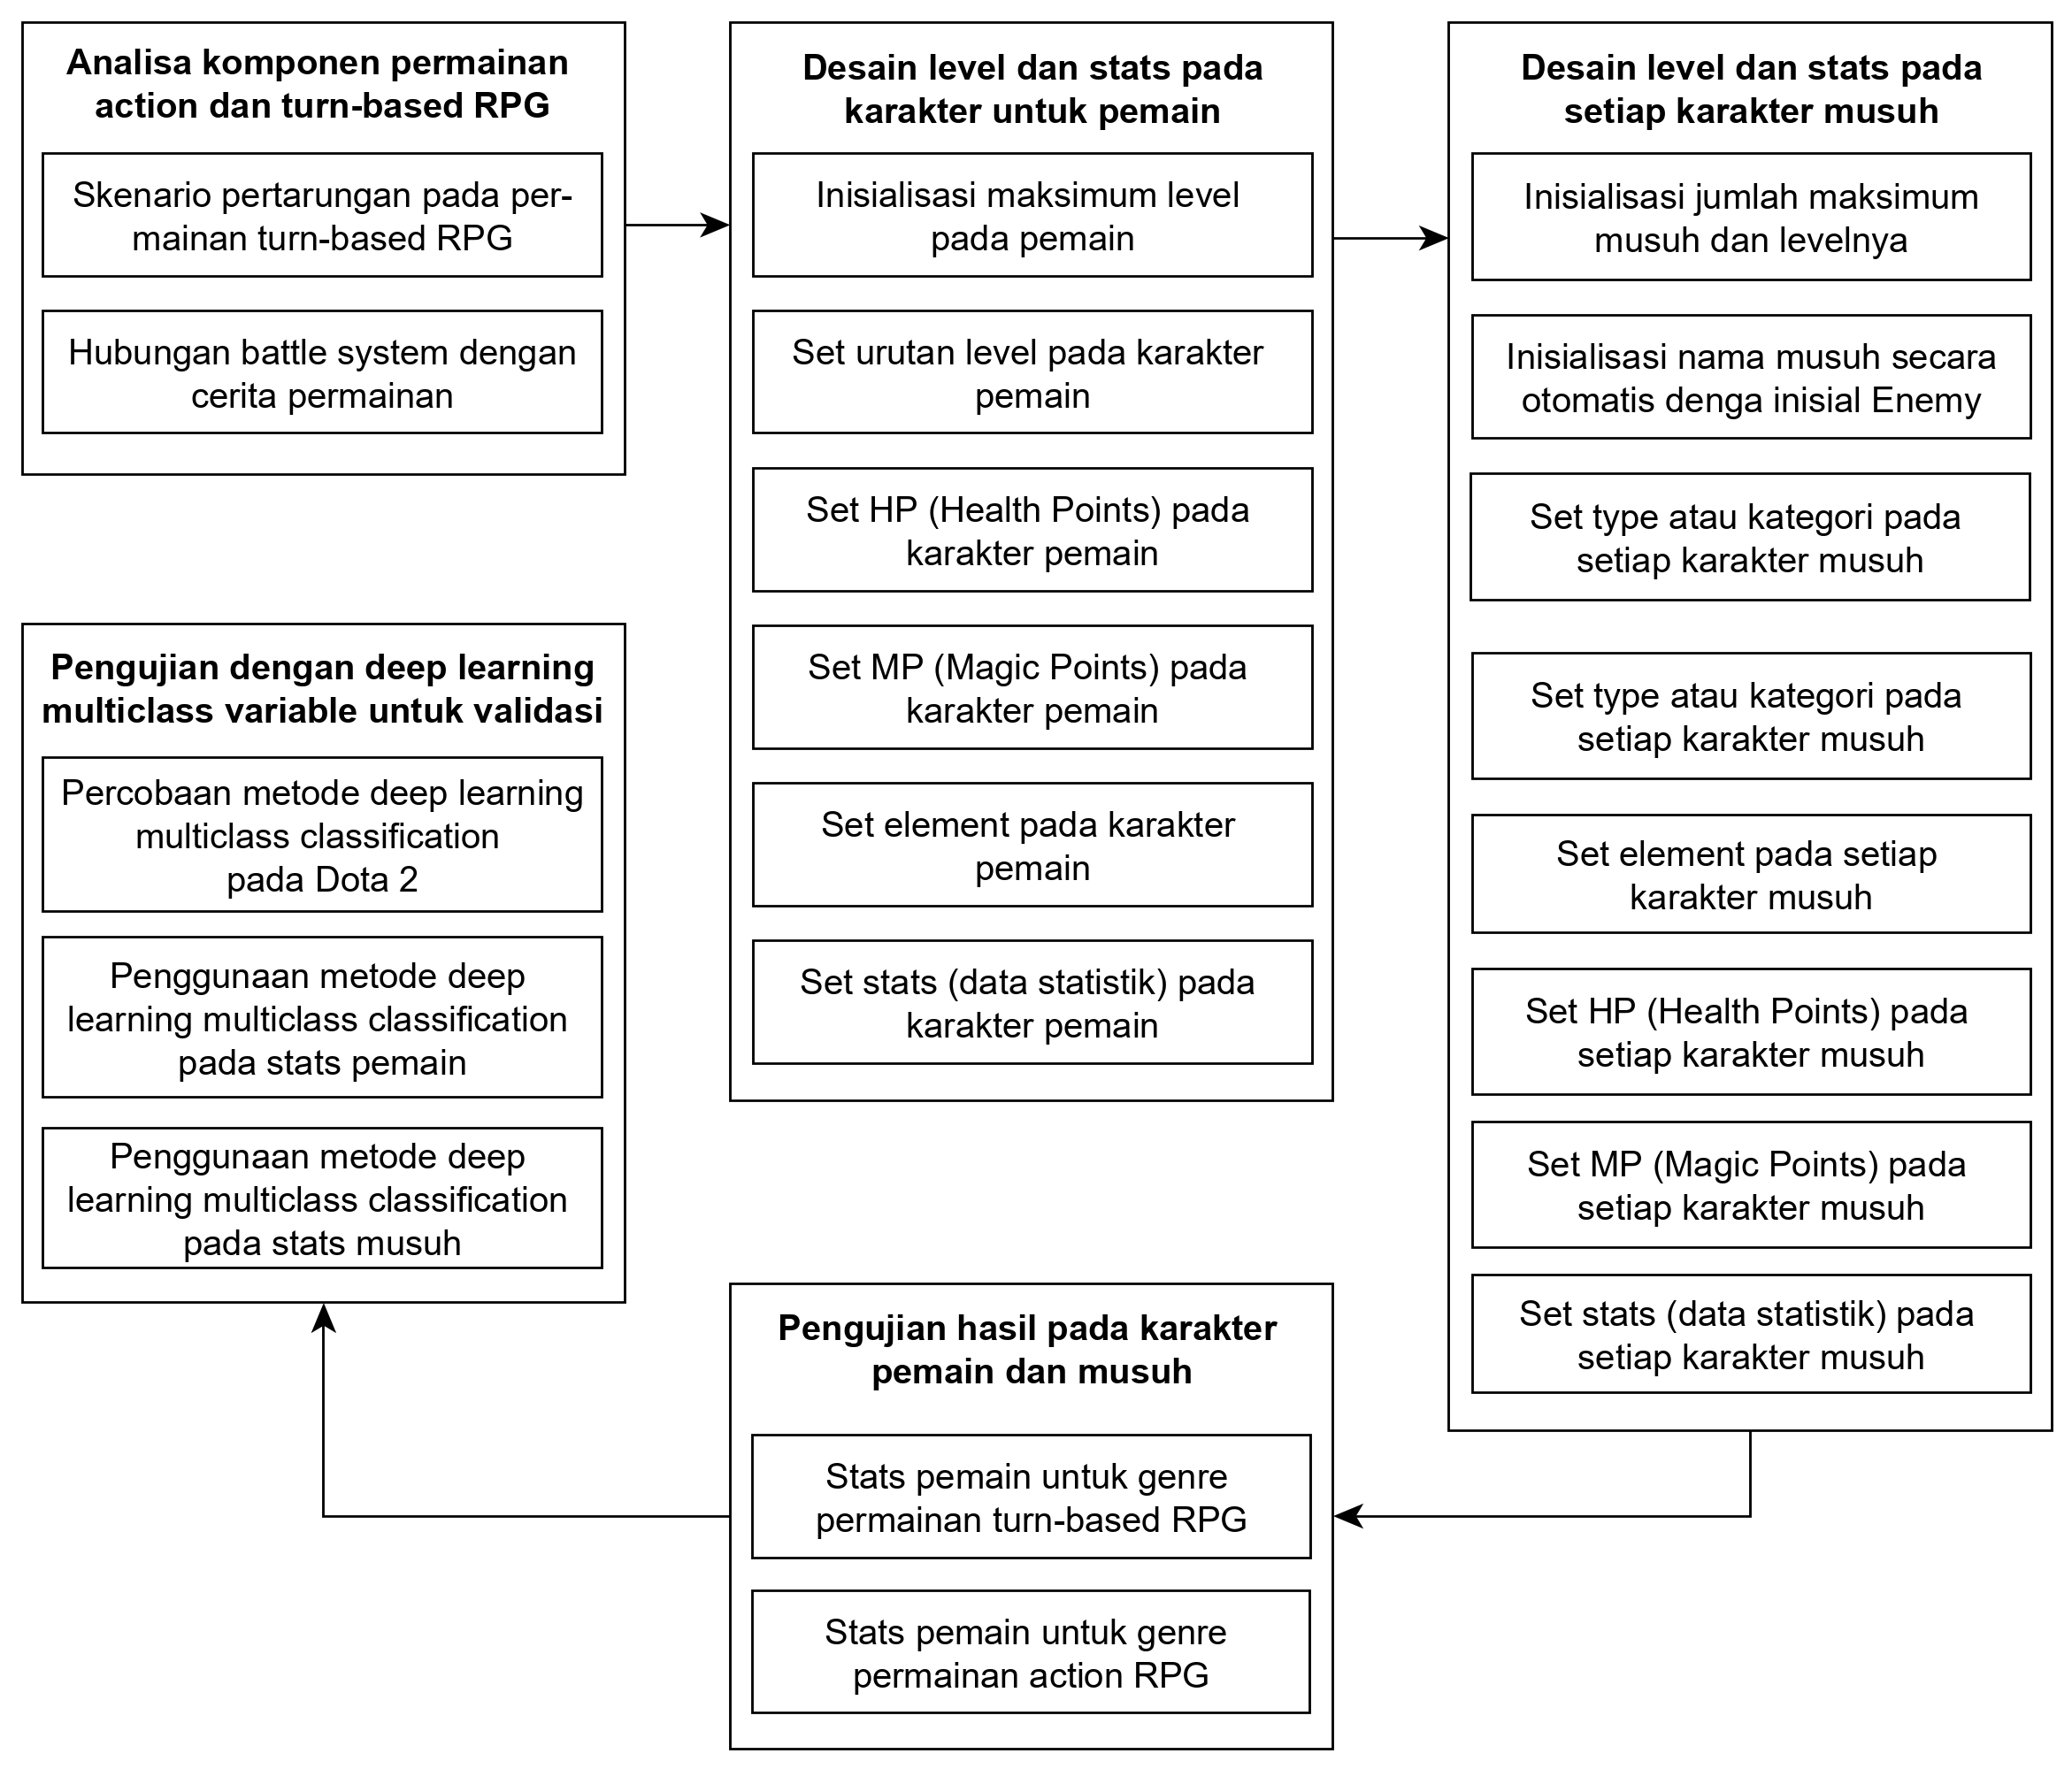
\includegraphics[scale=0.17]{img/metodologi_new.png}
	\caption{Urutan metodologi.}
	\label{fig:metodologi_2}    
\end{figure}

Tujuan umum dari penelitian ini adalah membuat \textit{stats} atau statistik untuk pemain dan musuh, sehingga dalam pembuatan permaian. Tujuan khusus dan fokus pada penelitian ini adalah untuk membuat data statistik untuk karakter pemain dan musuh dengan menggunakan metode $k-$NN dan \textit{Naive Bayes} yang kemudian dilakukan validasi dengan menggunakan metode \textit{Deep Learning} (\textit{Multiclass Classification}).
\vspace{1ex}

\section{Analisa Komponen Permainan Action dan Turn-based Role-Playing Game (RPG)}
\label{sec:sec3_design_komponen}
\vspace{1ex}

Pada bagian ini terdapat beberapa langkah yang akan menjelaskan penyusunan skenario pertarungan pada permainan RPG \textit{turn-based}. Pertama yang akan dilakukan adalah pembuatan skenario pertarungan pada permainan \textit{turn-based} RPG. Dari skenario tersebut tentunya harus ada hubungan dengan cerita dari permainan, apa saja parameter yang berpengaruh dari cerita terhadap skenario.
\vspace{1ex}

Di lanjutkan dengan desain level dan \textit{stats} dari pemain, selain itu digunakannya algoritma $k-$\textit{Nearest Neighbor} ($k-$NN) untuk mempercepat proses pembuatannya. Kemudian dilanjutkan dengan desain level dan \textit{stats} musuh yang juga dibuat secara otomatis dengan algoritma yang sama dengan pemain, namun tetap dipolakan oleh \textit{gaussian naive bayes} atau distribusi normal. 
\vspace{1ex}

Bagian selanjutnya adalah penambahan elemen pada pemain dan musuh yang membentuk kelebihan atau kekurangan pada masing-masing karakter. Pembagian elemen pada karakter yang dapat dimainkan oleh pemain dilakukan sesuai dengan cerita, sedangkan pembagian elemen pada musuh disebar secara acak berdasarkan \textit{stats} yang telah dibuat. Hal ini berkaitan erat dengan penjelasan pada Sub-bab \ref{sec:sub_sec2_kesempatan} tentang meningkatnya keberagaman, yang dibuktikan dengan banyaknya variasi musuh berikut dengan kelemahan dan kelebihannya.
\vspace{1ex}

\begin{subs}
	\subsection{Desain Skenario Pertarungan}
	\label{sec:sub_sec3_design_skenario}
	\vspace{1ex}
	
	Di umpamakan jumlah karakter yang rencananya akan digunakan berjumlah satu (\textit{action} RPG) sampai tiga karakter (\textit{turn-based} RPG) bergantung dengan alur cerita dari permainan dan jumlah musuh juga dimisalkan berjumlah antara satu sampai dengan enam, bergantung kepada tingkat kesulitannya seperti pada Gambar \ref{fig:battle_player}. 
	\vspace{1ex}
	
	\begin{figure} [!h] \centering
		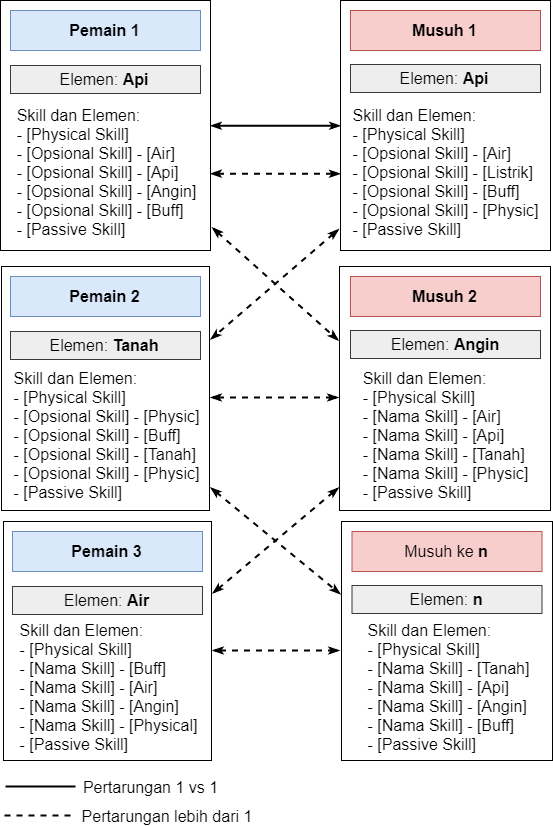
\includegraphics[scale=0.5]{img/battle_player_new.png}
		\caption{Skema pertarungan antar pemain.}
		\label{fig:battle_player}
	\end{figure}
	
	Sebelumnya pernah dijelaskan pada Sub-bab \ref{sec:sub_sec2_kesempatan} tentang meningkatnya pengambilan keputusan, pada kondisi semakin banyak musuh makan semakin banyak keputusan yang harus diambil oleh pemain. Selain itu setiap pemain memiliki elemen dan \textit{skill}, setiap elemen dapat menjadi kelemahan dan kelebihan dari setiap karakter. Hal tersebut akan membangun sebuah momen dramatis berdasarkan kompleksitas kombinasi dari musuh, hal tersebut dibahas pada Sub-bab \ref{sec:sub_sec2_kesempatan} tentang momen dramatis pada desain permainan.
	\vspace{1ex}
	
	Pada bagian ini dijelaskan contoh perancangan dari skenario pertarungan dengan genre \textit{action} dan \textit{turn-based} yang dibandingkan secara langsung. Pada Gambar \ref{fig:battle_player} jika dipecah dan dijelaskan lebih lanjut maka setiap karakter yang dimainkan oleh pemain atau musuh dalam bentuk NPC (\textit{Non Playable Character}) maka bagian-bagian tersebut akan menjadi seperti beberapa poin dibawah ini.
	\vspace{1ex}
	
	\begin{enumerate}[label=\textbf{\arabic*).}]
		
		\item \textbf{Stats}
		\setlength{\parindent}{0.8cm}
		
		\textit{Stats} atau statistik yang diperhitungkan dan berpengaruh dalam proses pertarungan. Pada Gambar \ref{fig:rpg_turn_based} ditunjukan tidak hanya karakter pemain saja, melainkan status dari pemain saat melakukan pertarungan. Pada Gambar \ref{fig:player_stats} adalah penggambaran dari komponen atau \textit{stats} pemain yang lebih detail seperti \textit{Health Point} (HP), \textit{Attack} atau serangan, \textit{Defense} atau pertahanan, \textit{Speed} atau kecepatan.
		\vspace{1ex}
		
		\begin{figure} [!h] \centering
			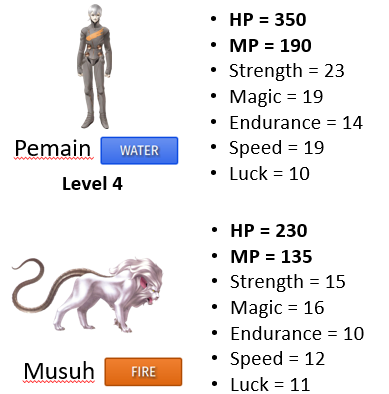
\includegraphics[scale=0.68]{img/player_stats.png}
			\caption{Status dari pemain pada permainan \textit{turn-based}.}
			\label{fig:player_stats}
		\end{figure}
		
		Berikut adalah penjabaran lebih dari beberapa komponen seperti HP, \textit{Attack}, \textit{Defense}, \textit{Speed} yang terdapat pada Gambar \ref{fig:rpg_turn_based}.
		
		\begin{enumerate}[label=\alph*).]
			\item \textbf{Health Point (HP)} adalah indikator nyawa atau kehidupan dari pemain, jika HP bernilai 0 maka karakter tersebut akan mati atu kalah.
			
			\item \textbf{Magic Point (MP)} adalah indikator jumlah dari jurus yang dapat dikeluarkan oleh pemain, jika MP bernilai 0 maka karakter tersebut tidak bisa mengeluarkan jurus atau kemampuan khusus.
			
			\item \textbf{Strength} adalah jumlah atau nilai serangan yang akan dilakukan untuk mengalahkan pemain lawan. Angka tersebut akan berlawanan atau dibandingkan dengan jumlah \textit{endurance} musuh. Hal tersebut bertujuan untuk mengurangi HP dari musuh.
			
			\item \textbf{Magic} atau \textit{Special Attack} biasanya tidak dimiliki oleh semua karakter pada permainan berbasis \textit{turn-based}. \textit{Special Attack} biasanya menjadi pembeda dalam setiap karakter berdasarkan jenis serangannya. Misalkan pada \textit{strength} biasanya berupa serangan fisik sedangkan pada \textit{special attack} berupa serangan \textit{magic} atau sihir.
			
			\item \textbf{Endurance} adalah jumlah atau nilai ketahanan yang digunakan oleh pemain atau musuh dalam menerima serangan. Hal ini bertujuan agar mencegah penurunan HP secara segnifikan, dengan membandingkan nilai serangan dengan nilai pertahanan.
			
			\item \textbf{Speed} atau kecepatan ada juga yang menyebutnya dengan \textit{agility} bertujuan dalam menentukan giliran dan keberhasilan dalam melakukan serangan. Semakin tinggi nilai \textit{speed}, biasanya semakin cepat melakukan serangan atau dapat mulai melakukan serangan lebih awal dibandingkan pemain atau musuh dengan nilai \textit{speed} yang lebih kecil.
			
			\item \textbf{Luck} atau keberuntungan adalah sebuah variabel yang digunakan menentukan hal yang bersifat acak, seperti bonus serangan atau \textit{critical attack}, kesempatan saat melakukan serangan balik atau \textit{counter attack} setelah diserang.
		\end{enumerate}
		
		Sementara itu skenario pertarungan dengan melibatkan \textit{stats} dijelaskan pada Gambar \ref{fig:battle_system} yang mana pemain atau musuh melakukan serangan berdasarkan \textit{speed}. Semakin tinggi \textit{speed} maka akan memperoleh giliran pertama untuk menyerang.
		\vspace{1ex}
		
		Di lanjutkan lagi dengan perhitungan dengan membandingkan \textit{Speed}, dan \textit{Luck} antara karakter pemain dengan musuh, pada proses tersebutlah yang menentukan apakah serangan dari pemain dapat diterima atau meleset terhadap musuh dan sebaliknya. Tingginya \textit{Speed} pada masing-masing karakter dapat diartikan perbandingn antara kecepatan untuk menyerang dan menghindar, sedangkan \textit{Luck} adalah faktor keberuntungan yang mempengaruhi serangan tersebut. Kemudian dilanjutkan lagi dengan kalkulasi \textit{attack} dan \textit{defense} antara karakter yang menyerang dan target. Dari hasil kalkulasi tersebut akan berpengaruh pada jumlah HP dari karakter yang menjadi target.
		\vspace{1ex}
		
		Kemudian pada permainan RPG dengan genre \textit{action} tidak membutuhkan skema berurutan serumit \textit{turn-based}. Pada permainan tersebut lebih mengandalkan ketangkasan dari pemain dalam memainkan karakter yang ingin dimainkan sepeti yang dijelaskan pada Sub-bab \ref{sec:sub_sec2_strategi} pada bagian pemain berbasis keterampilan sepenuhnya. Maka terjadilah momen saling serang secara langsung antara pemain dan musuh.
		\vspace{1ex}
		
		\begin{figure} [!h] 
			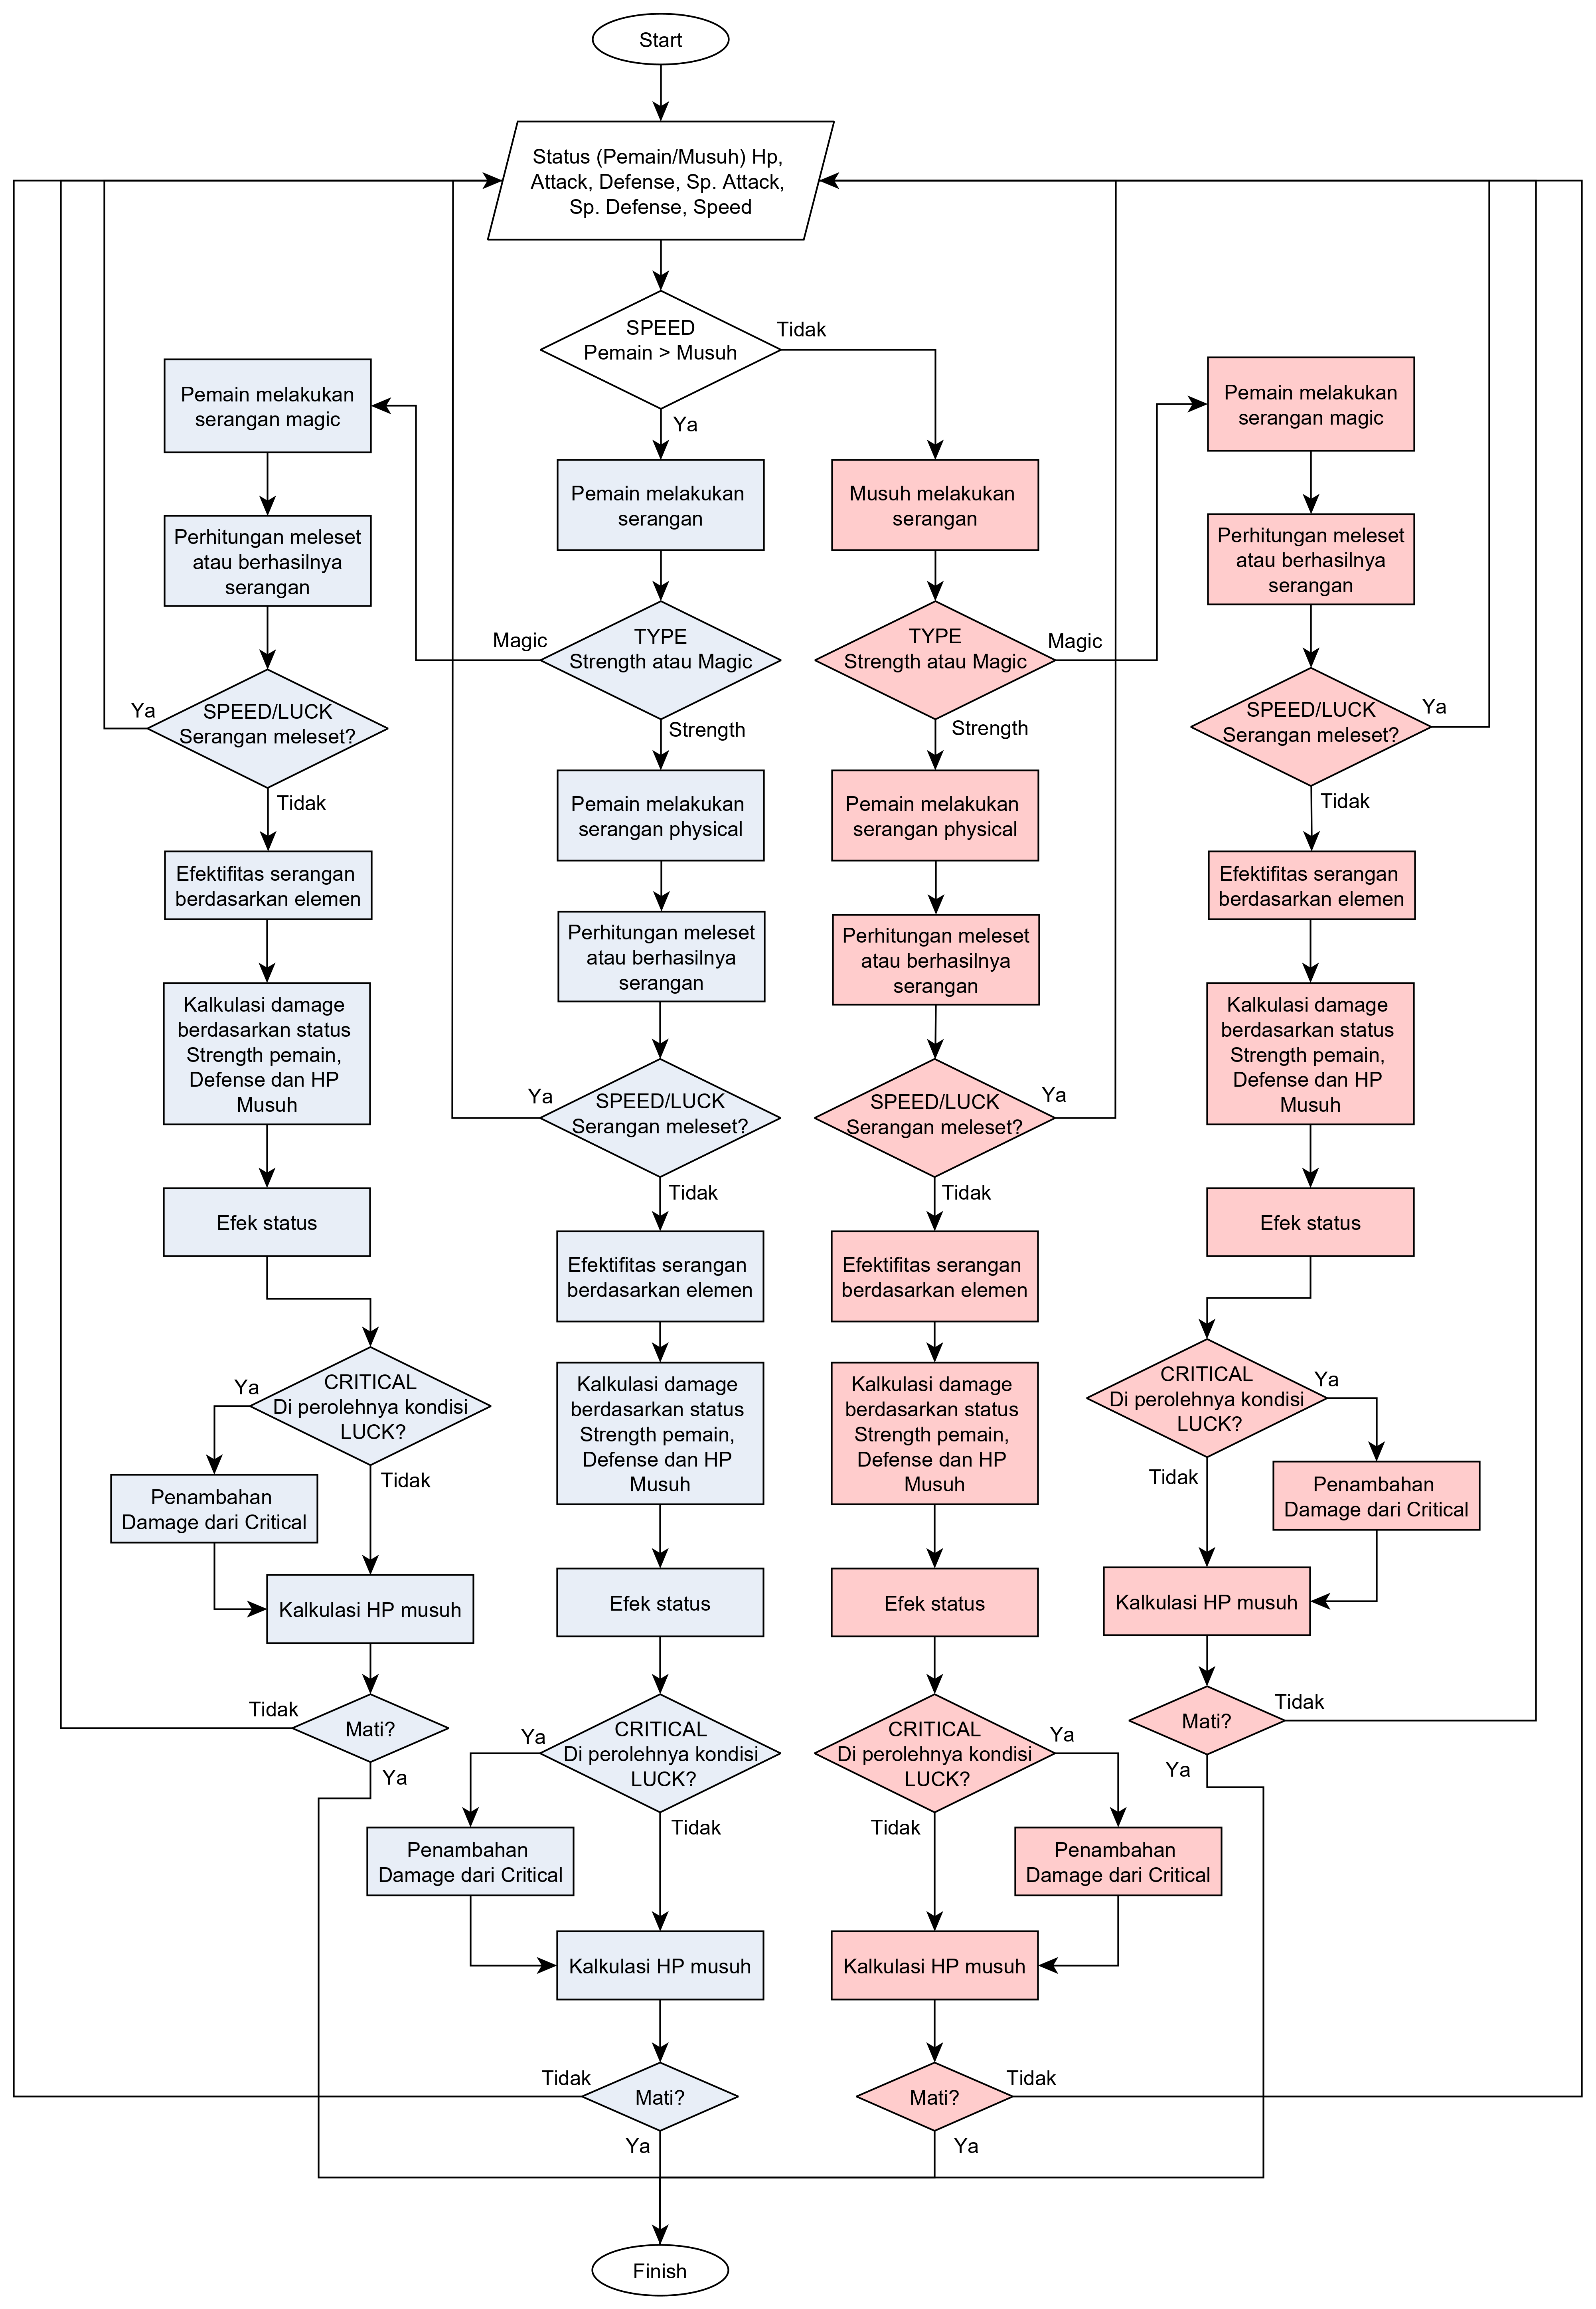
\includegraphics[scale=0.105]{img/battle_system_new_new.png}
			\caption{Skenario pertarungan \textit{turn-based}.}
			\label{fig:battle_system}
		\end{figure}
		\vspace{1ex}
		
		\item \textbf{Elemen dan Efektifitas Serangan}
		
		Pada Gambar \ref{fig:elemen} adalah contoh elemen yang digunakan dalam permainan dengan mode \textit{turn-based}. Jumlah dari elemen dapat ditambah atau dikurangi sesuai dengan kebutuhan. Biasanya jumlah dari elemen ditentukan berdasarkan cerita. Mengapa terdapat elemen tersebut, bagaimana asal-usulnya dan sebagainya seperti yang dijelaskan pada Sub-bab \ref{sec:sub_sec3_story}.
		\vspace{1ex}
		
		\begin{figure} [!h] \centering
			
\includegraphics[scale=0.45]{img/element.png}
			\caption{Elemen pada permainan dengan mode pertarungan \textit{turn-based}.}
			\label{fig:elemen}
		\end{figure}
		
		Pembahasan ini mengacu kepada Gambar \ref{fig:battle_system} pada bagian ``efektifitas serangan berdasarkan elemen". Sedangkan pada Gambar \ref{fig:efektifitas} adalah perbandingan pengaruh atau keterkaitan sebuah elemen dengan elemen yang lain. Di mana setiap elemen memiliki kelemahan yang berupa elemen lain dan sebaliknya. Elemen-elemen tersebut saling berlawanan satu dengan yang lainnya sehingga mampu membentuk sebuah permainan yang membutuhkan strategi khusus. Kemudian dilanjutkan dengan perhitungan \textit{stats} seperti bagian sebelumnya.
		\vspace{1ex}
		
		\begin{figure} [!h] \centering
			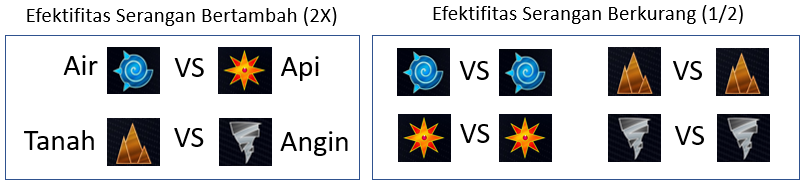
\includegraphics[scale=0.65]{img/efektifitas.png}
			\caption{Pengaruh elemen pada efektifitas serangan.}
			\label{fig:efektifitas}
		\end{figure}
		
		Jika melihat pada Gambar \ref{fig:efektifitas} dapat disimpukan bahwa beberapa element yang saling berlawanan kemudian efektifitas menjadi 2 kali lipat, contohnya pada elemen air terhadap api dan tanah terhadap angin begitu juga sebaliknya. Jika elemen yang sama saling bertarung maka efektifitasnya berkurang $1/2$ dari yang seharunya. Kemudian pada elemen lain yang belum disebutkan berlaku efektifitas normal atau 1 kali. Pembagian elemen pada pemain dan musuh akan dibahas lebih detail pada Sub-bab \ref{sec:sec3_player_stats}.
		\vspace{1ex}
		
		Kebanyakan elemen dan efektifitas serangan berlaku pada permainan RPG dengan genre \textit{turn-based}, berbeda halnya dengan \textit{action} yang lebih mengandalkan keterampilan dari pemain dalam memaikan karakternya seperti yang dijelaskan pada Sub-bab \ref{sec:sub_sec2_strategi} pada bagian pemain berbasis keterampilan sepenuhnya.
		\vspace{1ex}
		
		\item \textbf{Efek Status}
		
		Pada Gambar \ref{fig:battle_system} terdapat bagian ``efek status", maksud dari proses tersebut adalah penambahan efek yang merugikan terhadap pemain setelah diserang. Efek kerusakan dapat membawa kesan lebih taktis pada pertempuran. Berikut adalah efek status yang akan diterapkan pada sistem pertarungan.
		
		\begin{enumerate}[label=\alph*).]
			\item \textbf{Infected:} Karakter kehilangan 10\% dari total HP setiap giliran.
			
			\item \textbf{Confused:} Karakter tidak dapat dikendalikan dan mungkin akan bertahan, menyerang dan tidak melakukan apa-apa. Ada juga kemungkinan mereka akan berbalik menyerang \textit{party member} mereka sendiri.
			
			\item \textbf{Silence:} Karakter tidak dapat mengubah Personae atau menggunakan keterampilan Persona.
			
			\item \textbf{Tired:} Karakter kehilangan SP untuk setiap tindakan yang diambil, dan menerima lebih banyak \textit{damage} dari musuh ketika diserang.
			
			\item \textbf{Hacked:} Efek yang muncul setelah target diserang sesuai dengan kelemahannya. Target kemudian akan menerima lebih banyak \textit{damage} dan tidak dapat menghindar. Jika target diserang lagi, maka statusnya akan berubah menjadi disabled.
			
			\item \textbf{Disabled:} Target akan hilang 1 giliran untuk mengambil tindakan, kemudian mendapat lebih banyak kerusakan dan serangan tidak dapat dihindari.
		\end{enumerate}
		
		Tidak semua kemampuan pemain dapat memberi efek status, hal tersebut mengacu pada desain permainan yang mengatur keseluruhan \textit{skill}, tidak hanya pada karakter utama melainkan juga pada musuh. Tetapi dalam penelitian ini, hal tersebut masih belum terpakai dikarenakan masih menyelesaikan perihal desain \textit{stats} dari pemain dan musuh. Hal ini baru semacam perkiraan saja saat mendesain sebuah permainan.
		\vspace{1ex}
		
		Pada bagian efek status juga berlaku pada permainan RPG dengan genre \textit{action}, setelah berlangsungnya pertarungan antara pemain dan musuh. Di mana pada sisi pemain dapat memhangun karakternya sedemikian hingga demi memberi efek status ke pada musuh saat berlangsunnya pertarungan seperti yang dijelaskan pada Sub-bab \ref{sec:sub_sec2_strategi} tentang peran dan keterampilan pemain serta strategi dan taktik.
		\vspace{1ex}
		
		\item \textbf{Kondisi Kritis pada Serangan}
		
		Selain \textit{attack}, elemen dan efek status, masih terdapat \textit{damage} yang dapat ditimbulkan oleh penyerang kepada target yaitu kondisi kritis pada serangan. Dengan jumlah \textit{attack} ditambah dengan jumlah \textit{attack} yang dikalikan dengan presentase tingkat kondisi kritis (\textit{critical rate}) pada \textit{skill} yang dipilih untuk menyerang lawan. Kondisi tersebut didapat dengan membandingkan nilai \textit{stats} dari \textit{Strength} atau \textit{Magic} dan \textit{luck} milik penyerang dan target, pada proses tersebutlah yang menentukan apakah serangan tersebut diperoleh kondisi kritis atau tidak. Hal tersebut juga membangun sebuah momen dramatis berdasarkan peluang terjadinya kondisi kritis saat terjadinya serangan dari pemain terlebih lagi dari musuh seperti yang dibahas pada Sub-bab \ref{sec:sub_sec2_kesempatan} tentang momen dramatis.
		\vspace{1ex}
		
		\item \textbf{Kalkulasi HP dan MP}
		
		Pada akhirnya jumlah kerusakan yang ditimbulkan oleh penyerang dan HP dari target akan dikalkulasikan. Jika HP target habis atau sama dengan 0, maka terget tersebut dinyatakan mati. Dan jika HP target masih bersisa, maka pertarunggan akan dilanjutkan oleh giliran karakter dari pemain atau musuh selanjutnya. Kemudian pada sisi penyerang juga ada yang dikorbankan dalam upaya melakukan serangan. Saat penyerang memilih serangan fisik makan pemain akan mengorbanakan sebagian HP yang dimiliki, jika yang dipilih adalah serangan \textit{magic} maka yang dikorbankan adalah MP.
	\end{enumerate}
	
	\subsection{Hubungan Sistem Pertarungan dengan Cerita}
	\label{sec:sub_sec3_story}
	\vspace{1ex}
	
	Pada setiap permainan RPG khususnya \textit{action} dan \textit{turn-based} RPG pasti memiliki cerita yang menjadi latar belakang permainan seperti yang dijelaskan pada Sub-bab \ref{sec:sec2_turn_based_rpg}. Tentunya cerita tersebut juga memiliki pengaruh penting terhadap jumlah karakter yang dapat dimainkan oleh pemain, jumlah musuh, elemen apa saja yang akan dipakai, total waktu permainan, jumlah musuh yang harus dilawan dan lain sebagainya. Pada penelitian ini hal semacam itu akan dibuat menjadi sebuah estimasi yang kemudian disimulasikan ke dalam mode pertarungan dengan berbagai macam estimasi sebagaimana penjelasan berikut.
	\vspace{1ex}
	
	\begin{enumerate}[label=\textbf{\arabic*).}]
		
		\item \textbf{Tingkat Kesulitan Musuh}
		\setlength{\parindent}{0.8cm}
	
		Berikut adalah beberapa pertanyaan yang harus ditanyakan kepada setiap pembuat desain permainan:
		
		\begin{enumerate}[label=\alph*).]
			\item Haruskah kebanyakan pemain nantinya dapat menyelesaikan permainan tanpa melakukan \textit{side quest} (misi sampingan) atau melakukan \textit{grinding} (menaikan kemampuan karakter) diluar standar perkembangannya?
			\item Berapa banyak bos yang akan dilawan oleh pemain pada permainan ini, dan seberapa jauh jaraknya? Dan bagaimana dengan penambahan bos?
			\item Berapa banyak \textit{dungeon} (tempat muncul dan bertemu dengan musuh) yang akan disajikan, dan seberapa besar \textit{dungeon} tersebut?
			\item Akankah pemain bisa menyimpan progres permainan kapan saja, atau hanya di titik penyimpanan tertentu yang sudah ditentukan?
		\end{enumerate}
		\vspace{1ex}
	
		Biasanya pada permaianan \textit{turn-based} RPG terdapat sebuah peta besar tentang lokasi yang merupakan latar dari cerita, tersebarlah berbagai jenis musuh yang relatif mudah dikalahkan. Kemudian ditampilkan juga beberapa \textit{dungeon} yang akan terbuka satu demi satu, yang mana \textit{dungeon} tersebut memiliki tingkat kesulitan dan kerumitan yang terus meningkat sampai dengan bertemu dengan Bos. Secara keseluruhan tingkat kesulitan juga akan terus meningkat sampai dengan akhir permaian seperti yang dicontohkan oleh Gambar \ref{fig:story_dungeon}.
		
		\begin{figure} [!h] \centering
			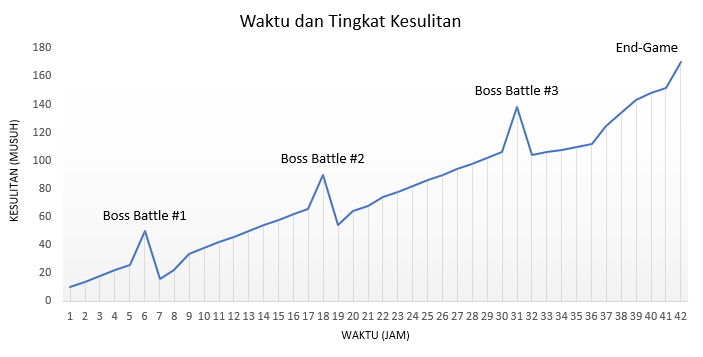
\includegraphics[scale=0.68]{img/story_dungeon.png}
			\caption{Pengaruh cerita terhadap tingkat kesulitan.}
			\label{fig:story_dungeon}
		\end{figure}
		
		Adapun beberapa cara untuk meminimalisir \textit{grinding} dan lamanya waktu permainan, dengan diberikan Exp (\textit{Experience} adalah sebuah variabel untuk pemain agar naik level) kepada pemain untuk menyelesaikan misi dan mengalahkan musuh yang lebih sulit dari pada mengalahkan musuh yang relatif mudah ditaklukan yang tersebar pada peta. Tentu saja musuh yang tersebar di peta juga memberikan Exp bagi pemain, namun seiring bertambahnya level pemain maka Exp yang diperoleh saat melawan musuh dengan level rendah akan semakin kecil.
		\vspace{1ex}
		
		Pada penelitian ini tingkat kesulitan langsung disimulasikan dengan pertarungan antara karakter-karakter yang dimainkan oleh pemain melawan musuh, dengan kondisi tingkat kesulitan musuh yang terus naik lalu turun kemudian naik lagi dan turun lagi, naik lagi dan seterusnya sampai dengan kondisi puncak. Hal ini mensimulasikan kondisi yang dilalui oleh pemain saat melawan \textit{trash mobs}, memasuki \textit{dungeon}, saat bertarung melawan bos dan kemudian pada akhirnya bertarung melawan bos terakhir. Lebih detailnya akan dijelaskan pada poin selanjutnya.
		\vspace{1ex}
	
		\item \textbf{Waktu yang Diperlukan untuk Kalahkan Musuh}
	
		Musuh pada permainan \textit{turn-based} RPG umumnya terbagi menjadi empat kategori diantaranya adalah:
		
		\begin{enumerate}[label=\Alph*).]
			\item \textit{Trash Mobs} adalah musuh yang tersebar pada seluruh area atau map.
			\item \textit{Dungeon Mobs} dapat dibagi menjadi dua sub-kategori:
			\begin{enumerate}[label=\alph*).]
				\item \textit{Dungeon Trash} atau sama seperti \textit{Trash Mobs} yang sebagian besar ditemukan awal sampai tengah \textit{dungeon}.
				\item \textit{Difficult Dungeon Trash} atau yang lebih sulit terletak lebih dekat ke bos atau dari tengah ke akhir \textit{dungeon}.
			\end{enumerate}
			\item \textit{Mini-Boss}/\textit{Boss Mobs}.
			\item \textit{End-Game Boss}/\textit{Secret Boss} (Bos yang bersifat opsional).
		\end{enumerate}
		
		Pada penelitian ini keseimbangan permainan dirancang terus meningkat seperti yang dibahas pada bagian sebelumnya, dalam permainan ini sebagian besar waktu (asumsikan saja 80\%) akan dihabiskan bertarung di dalam \textit{dungeon}. Kemudian 20\% dari waktu pertempuran akan digunakan untuk bertarung melawan bos. Sedangkan sisanya 60\% dari waktu bertarung akan dibagi antara pertarungan melawan musuh yang lemah dan juga kuat, bila digambarkan pembagian tersebut akan seperti pada Gambar \ref{fig:enemy_difficulty_percentage}.
		
		\begin{figure} [!h] \centering
			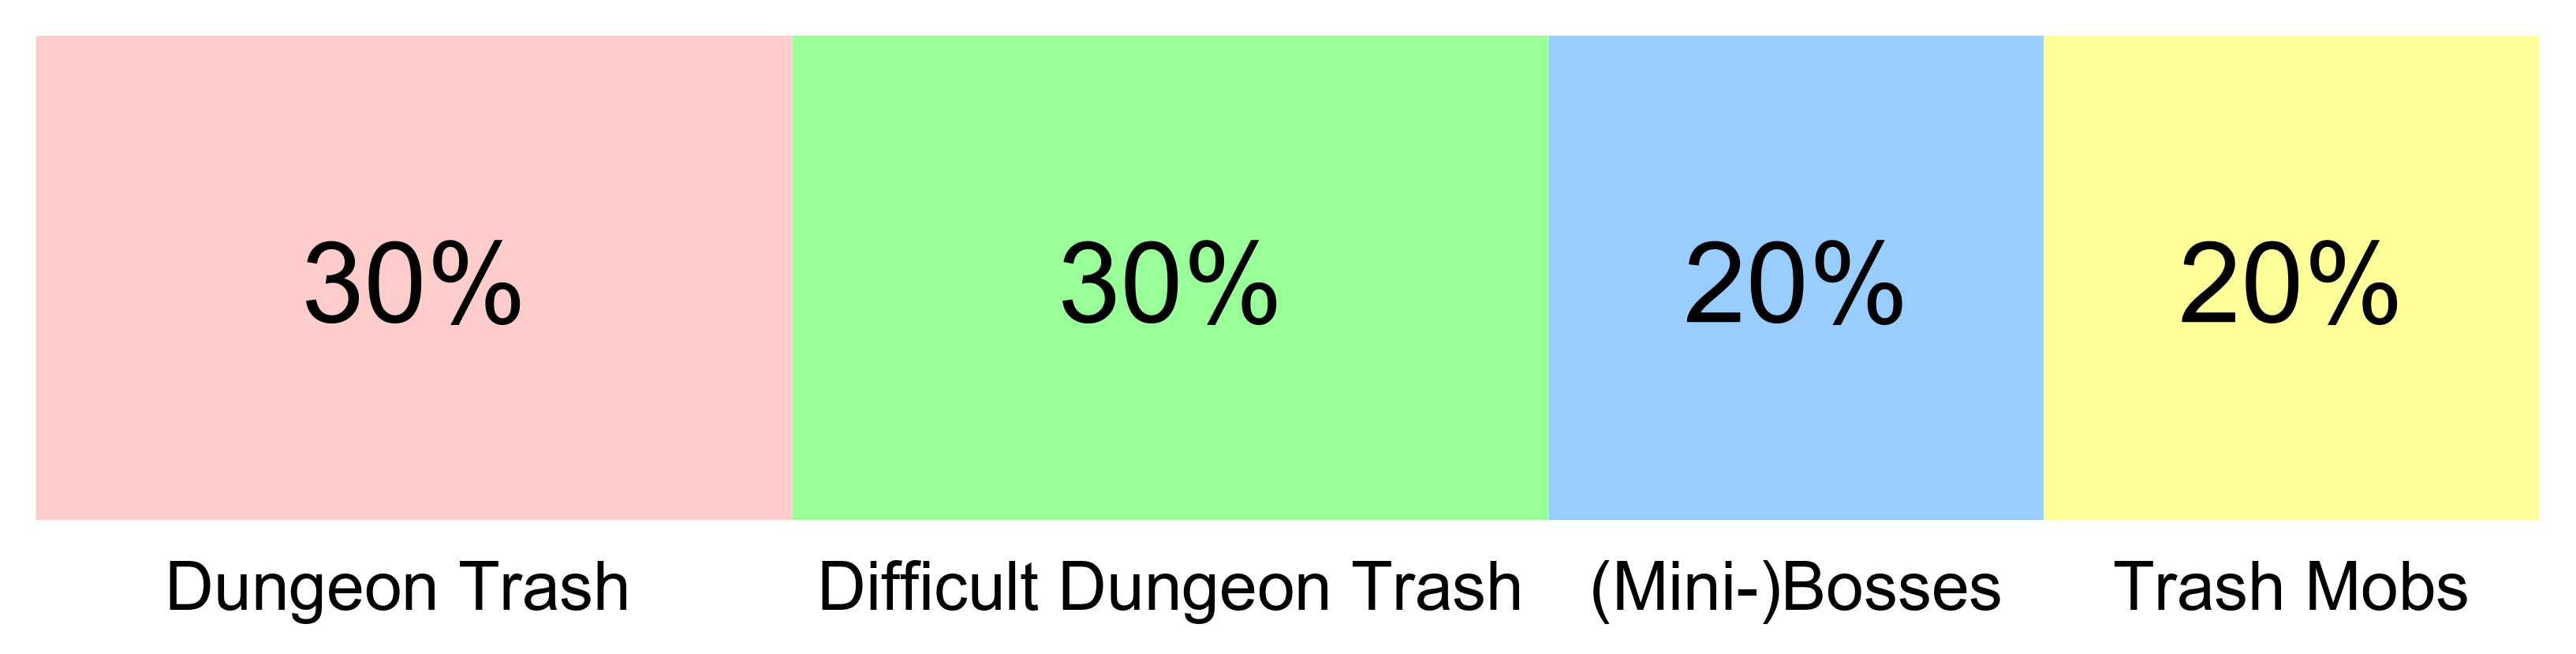
\includegraphics[scale=0.12]{img/enemy_type_distribution.png}
			\caption{Distribusi jenis musuh sesuai dengan cerita.}
			\label{fig:enemy_difficulty_percentage}
		\end{figure}
		
		Perhatikan bahwa dalam distribusi yang dibuat, jumlah waktu yang dihabiskan untuk melawan bos sama seperti waktu yang dibutuhkan untuk memerangi \textit{Thrash Mobs}. Dalam proses replikasi distribusi dalam permainan, pertama tentukan jumlah total waktu yang dibutuhkan oleh pemain untuk mengalahkan naga, raksasa atau apa pun yang biasanya disebut dengan bos.
		\vspace{1ex}
		
		Misalnya, dalam permaian RPG, bos pertama idealnya akan membutuhkan 3 menit bagi pemain yang kompeten untuk mengalahkan, dan bos terakhir menghabiskan waktu 20 menit. Kemudian terjadi peningkatan kompleksitas pada bos di level menengah, untuk terdapat dua bos yang masing-masing membutuhkan waktu sekitar 10 menit untuk dikalahkan, dan bos kedua membutuhkan waktu 7 menit.
		\vspace{1ex}
		
		\begin{equation}
		\label{eq: total_fight}
		B_{total} = \sum_{n = 0}^{k} B_{n}
		\end{equation}
		
		Merujuk ke persamaan \ref{eq: total_fight} bila dijabarkan maka $B_{total}$ adalah jumlah waktu melawan bos secara keseluruhan, jumlah bos dinyatakan dengan $k$ dan waktu yang dihabiskan untuk melawan satu bos dinyatakan dengan $B$ kemudian diiterasi oleh $n$ sejumlah $k$.
		\vspace{1ex}
		
		Di perlukannya penyesuaian terhadap model distribusi, salah satunya waktu yang habis untuk melawan bos setara untuk melawan musuh yang mudah atau \textit{trash mobs}. Untung saja terdapat banyak cara untuk memodifikasi waktu yang akan dihabiskan saat bertarung melawan musuh yang mudah. Hal seperti menjelajah seluruh peta atau berpetualang menuju tempat-tempat sebelumnya juga tidak perlu dilakukan. Berikut adalah langkah-langkah yang dapat dilakukan:
	
		\begin{enumerate} [label=\alph*).]
			\item  Mengurangi atau meningkatkan tingkat pertemuan dengan musuh yang mucul secara acak atau yang biasa disebut dengan \textit{random encounter rate}. Bisa juga dengan tingkat \textit{spawn} (muncul lagi setelah mati).
			\item Menambah atau mengurangi jumlah musuh saat pertempuran.
			\item Membatasi kemampuan musuh yang menimbulkan efek status yang menyulitkan dan menghabiskan waktu seperti \textit{confused}, \textit{silence}, \textit{tired} dan lain-lain.
			\item Menambah atau mengurangi kekuatan musuh.
			\item Menambah atau mengurangi kekuatan dari \textit{party member}.
		\end{enumerate}
	\end{enumerate}
\end{subs}

Terdapat banyak fleksibilitas di sini, developer dapat mengisi daftar musuh yang akan muncul secara acak dengan musuh yang sulit dikalahkan dengan tingkat probabilitas kemunculan yang kecil, atau lebih sering memunculkan musuh yang mudah dikalahkan. Alternatif lain adalah dengan meningkatkan kekuatan \textit{party member} atau jumlah rata-rata musuh yang bertarung dalam satu kali pertarungan. Kebebasan desain semacam ini yang nantinya akan memudahkan penyeimbangan permainan. Sedangkan jumlah musuh dan panjangnya level dari pemain atau musuh sendiri menggambarkan akan lamanya permainan tersebut. Pada dasarnya semua proses diatas mengacu pada pokok pembahasan dari referensi yang dibahas pada Sub-bab \ref{sec:sub_sec2_keseimbangan} tentang menemukan keseimbangan.
\vspace{1ex}

\section{Desain Level dan Stats pada Karakter Pemain}
\label{sec:sec3_player_stats}
\vspace{1ex}

Di buatlah sebuah program yang secara otomatis dapat membuat \textit{stats} dari pemain dengan masukan sesuai dengan kebutuhan desainer permainan atau developer. Program tersebut terdiri dari beberapa fungsi yang pada awalnya adalah obyek yang memiliki masukan parameter-parameter yang nantinya akan menghasilkan sebuah data yang berupa \textit{stats} dari karakter pemain seperti proses yang ditunjukan oleh diagram alur pada Gambar \ref{fig:player_stats_generator}.
\vspace{1ex}

\begin{figure} [!h] \centering
	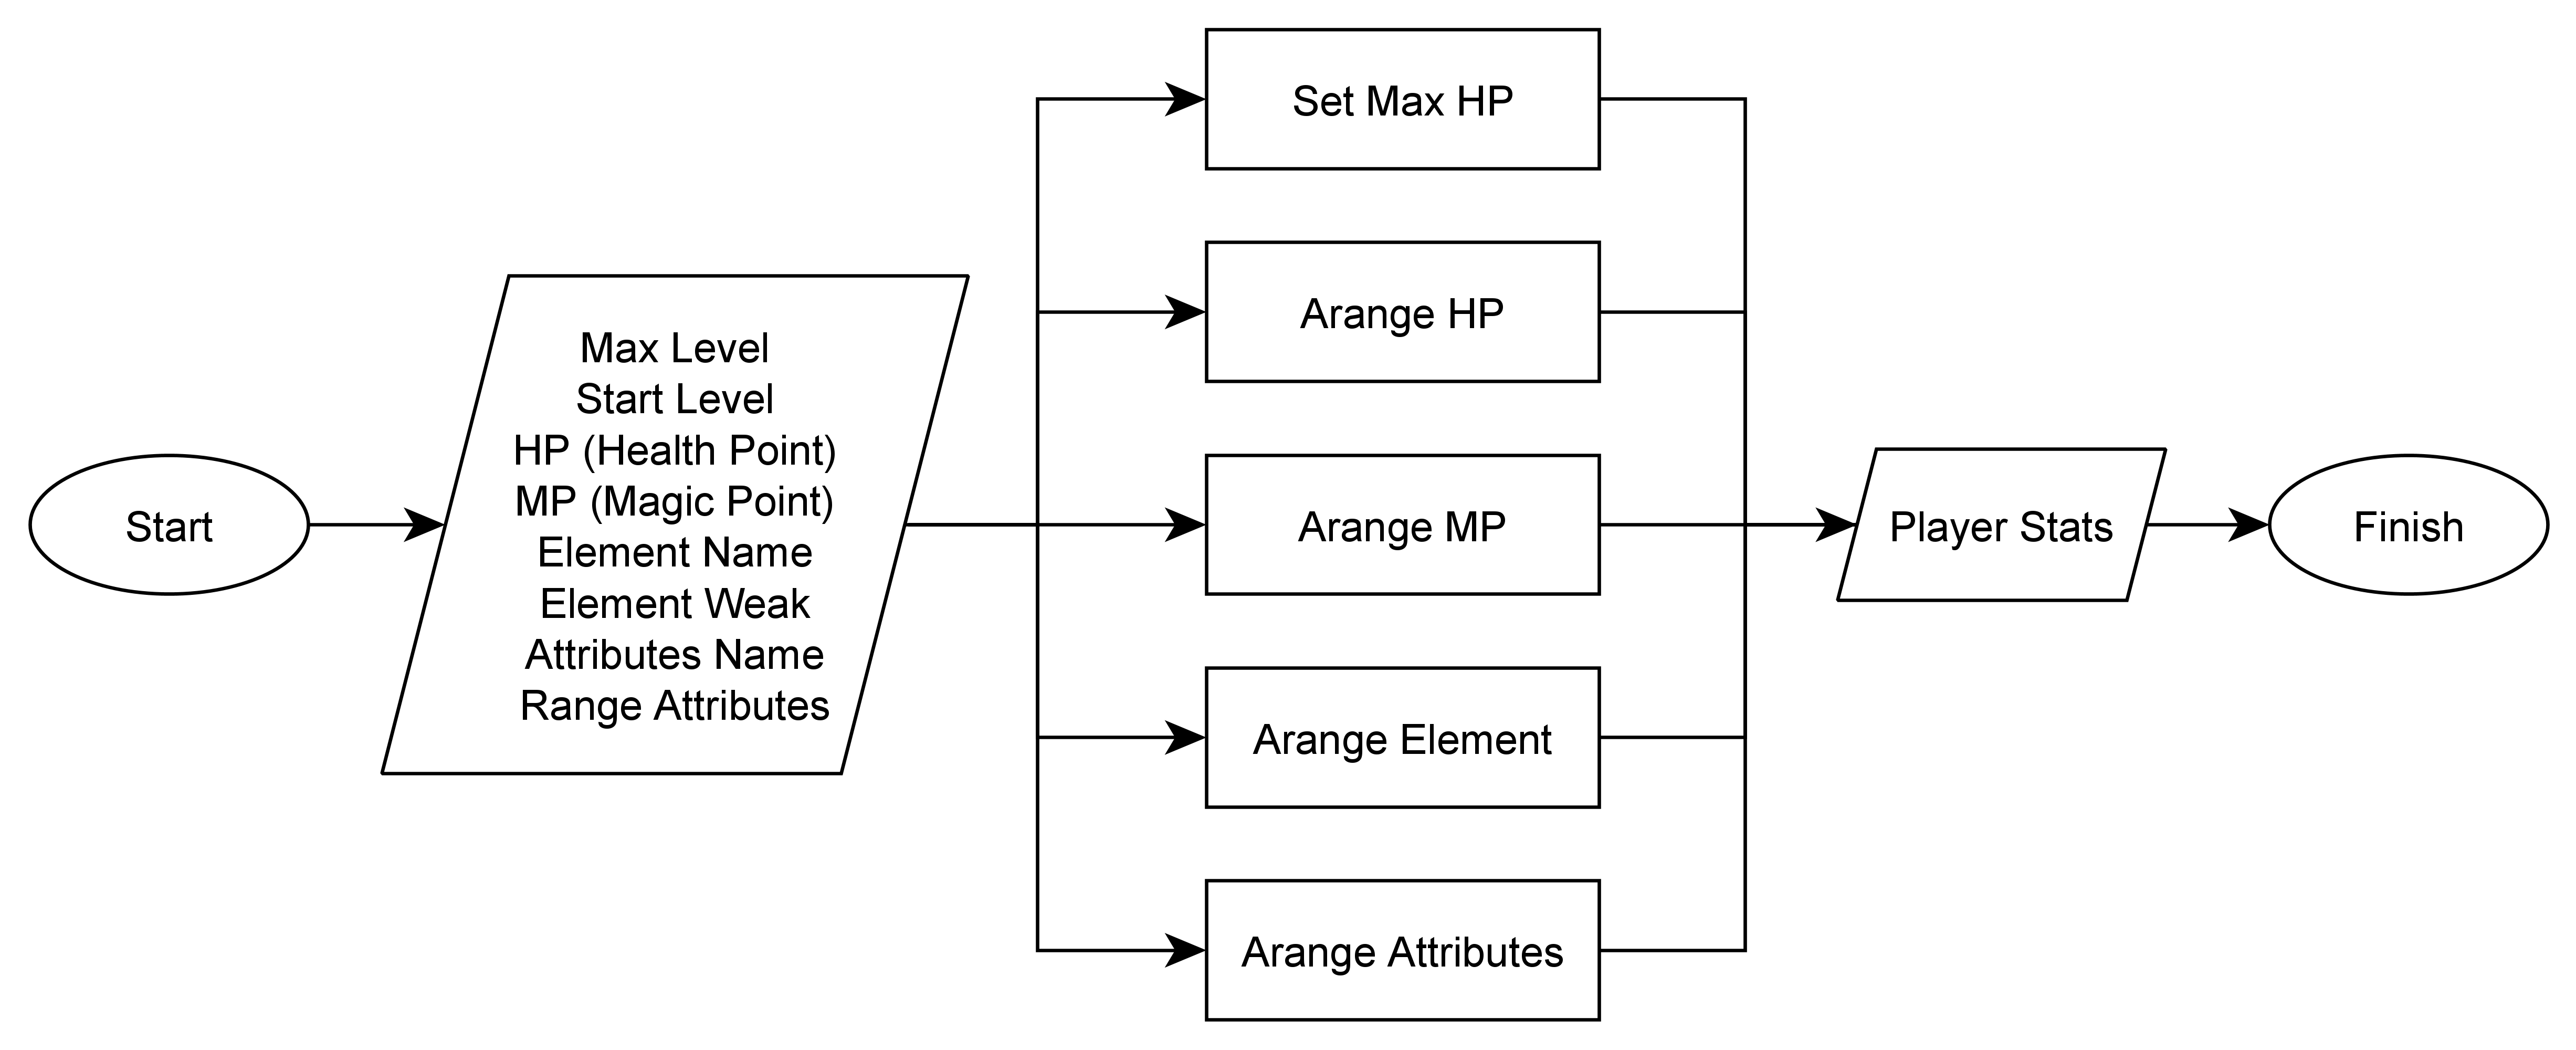
\includegraphics[scale=0.037]{img/player_stats_generator.png}
	\caption{Proses pembuatan stats untuk karakter pemain.}
	\label{fig:player_stats_generator}
\end{figure}

Pada permainan dengan genre \textit{turn-based} RPG dengan jumlah karakter yang dapat dimainkan berjumlah lebih dari satu, maka program yang ditunjukan melalui proses pada Gambar \ref{fig:player_stats_generator} akan dijalankan lebih dari satu kali. Hal tersebut dilakukan dengan tujuan agar karakter utama atau yang dapat dimainkan oleh pemain berjumlah lebih dari satu. Lain halnya dengan \textit{action} RPG, cukup hanya dengan satu kali menjalankan program maka sudah diperolehnya \textit{stats} dari karakter yang dibuat. Hal tersebut dikarenakan biasanya permainan dengan genre action RPG, jumlah karakternya hanya satu.
\vspace{1ex}

Pada Gambar \ref{fig:player_stats_generator} disisi masukan program terdapat banyak sekali masukan variabel seperti \textit{Max Level} yang berupa maksimum level yang di inginkan, kemudian \textit{Start Level} yang berupa level awal dari pemain, kemudian HP yang berupa \textit{range} atau jarak antara HP terendah dengan HP terendah setelah itu. Sama halnya dengan HP, dalam perhitungan \textit{range} atau jarak pada \textit{MP} juga menggunakan cara tersebut. Kemudian \textit{Element Name} berisi daftar elemen apa saja yang ingin digunakan, begitu juga dengan \textit{Name Stats}. Kemudian untuk \textit{Range Stats} berisikan \textit{stats} awal atau inisialisasi dan maksimum \textit{stats}. Lebih detail tentang program yang dibuat dapat dilihat pada Gambar \ref{fig:player_uml}, yang merupakan \textit{class} diagram untuk membuat \textit{stats} pemain.
\vspace{1ex}

\begin{figure} [!h] \centering
	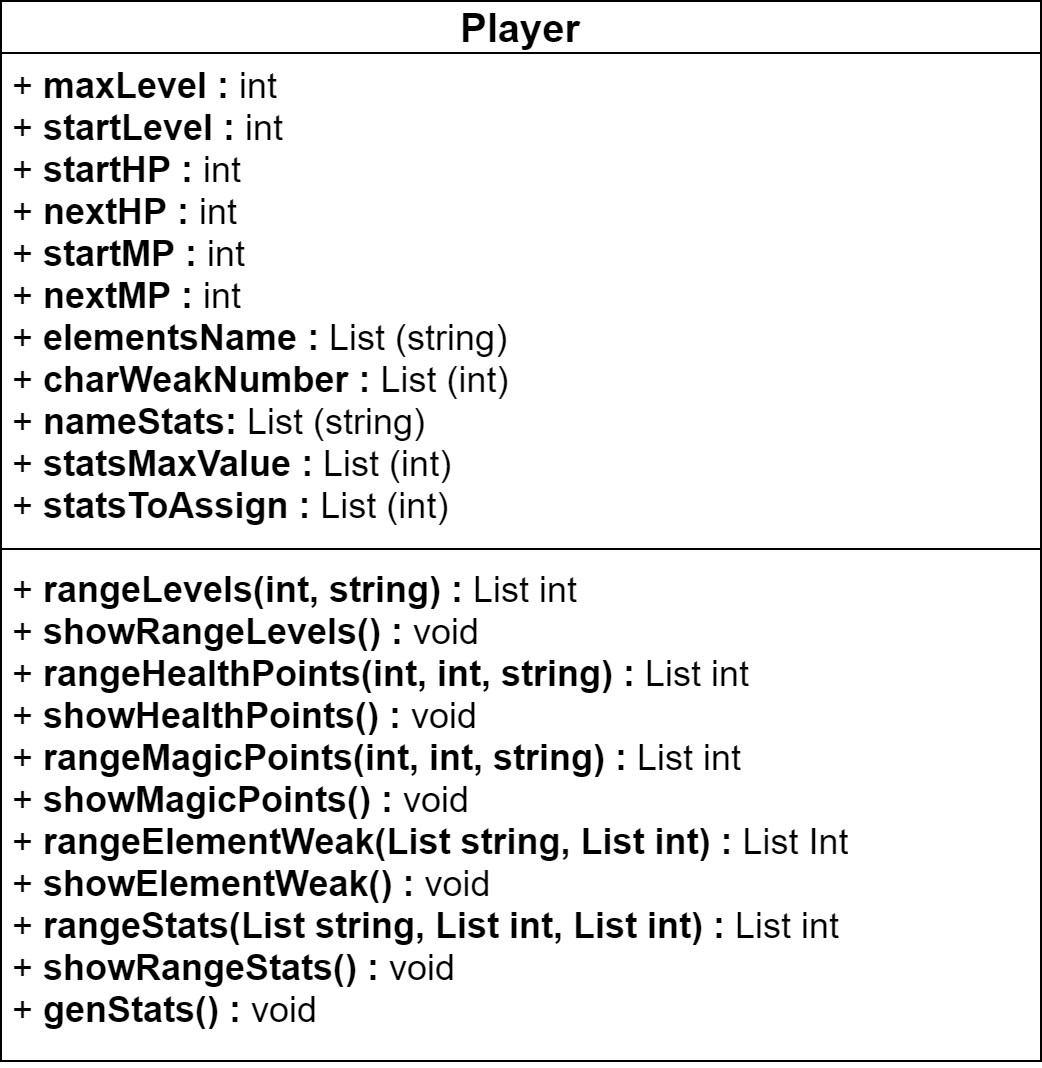
\includegraphics[scale=0.25]{img/player_uml.png}
	\caption{\textit{Class} diagram untuk \textit{stats} pemain.}
	\label{fig:player_uml}
\end{figure}

Karena program ini dibangun menggunakan OOP (\textit{Object Oriented Programming}) maka program ini dapat dijabarkan menggunakan Gambar \ref{fig:player_uml}. Selain itu program ini juga dapat secara mudah dimodifikasi untuk keperluan pengembangan kedepannya, dengan fungsi-fungsi yang ada sangat memungkinkan dilakukan \textit{override} atau pembuatan fungsi yang sama dengan isi atau proses yang berbeda.
\vspace{1ex}

Dalam menjelaskan proses pada BAB ini maka diambilah sebuah kasus dalam desain permainan, khususnya dalam penyusunan \textit{stats} untuk pemain dengan genre permaian \textit{turn-based} dan \textit{action} RPG. Pada Tabel \ref{tb:player_input_variable} adalah masukan untuk menguji program yang akan dijelaskan pada bagian selanjutnya, yang mana masukan pada Tabel \ref{tb:player_input_variable} akan menghasilkan \textit{stats} pada sebuah karakter untuk pemain.
\vspace{1ex}

\begin{table}[!h]
	\centering
	\caption{Data masukan untuk pembuatan \textit{stats} pemain.}
	\label{tb:player_input_variable}
	\begin{tabular}{|l|l|}
		\hline
		\rowcolor[HTML]{9B9B9B} 
		\multicolumn{1}{|c|}{\cellcolor[HTML]{9B9B9B}\textbf{Variabel}} & \multicolumn{1}{c|}{\cellcolor[HTML]{9B9B9B}\textbf{Input}} \\ \hline
		\textit{Max} Level & 100 \\ \hline
		\textit{Start} Level & 1 \\ \hline
		\textit{Start} HP & 159 \\ \hline
		\textit{Next} HP & 163 \\ \hline
		\textit{Start} MP & 89 \\ \hline
		\textit{Next} MP & 93 \\ \hline
		\textit{List Element} & {[} `Phys', `Water', `Wind', `Earth', `Fire' {]} \\ \hline
		\textit{List Weaknesess} & {[} 1, 2, 1, 1, 0 {]} \\ \hline
		\textit{List Stats Name} & {[} `Strength', `Magic', `Endurance', `Speed', `Luck' {]} \\ \hline
		\textit{Max Stats Value} & {[} 74, 38, 63, 65, 60 {]} \\ \hline
		\textit{Stats to Assign} & {[} 2, 1 {]} \\ \hline
	\end{tabular}
\end{table}
\vspace{1ex}

\subsection{Distribusi Level, HP dan MP Pemain}
\label{sec:sub_sec3_player_level_hp_mp}
\vspace{1ex}

Berdasarkan Tabel \ref{tb:player_input_variable} level untuk karakter pemain dimulai dari 1 dan level maksimalnya adalah 100, pada program ini level pemain akan terus naik satu demi satu level sampai ke tingkat maksimal. Selanjutnya adalah HP atau \textit{Health Point} yang diberi masukan berupa \textit{start} HP, bisa dinyatakan juga sebagai HP saat level satu. Kemudian variabel lanjutannya adalah \textit{next} HP atau HP pada level selanjutnya, misalkan level dua. Muncul sebuah pertanyaan berapa HP selanjutnya sampai dengan level ke 100. 
\vspace{1ex}

Cara semacam itu juga berlaku untuk perhitungan MP pada programm ini, dengan pola masukan yang sama dengan HP yaitu \textit{Start} MP dan \textit{Next} MP. Pada persamaan \ref{eq:hp_player} dan \ref{eq:mp_player} adalah contoh persamaan yang digunakan untuk mencari nilai HP dan MP selanjutnya.
\vspace{1ex}

\begin{equation}\label{eq:hp_player}
	\begin{split}
		HP(N) = \sum_{n = 0}^{N} HP(n + 1) + \left(HP(n + 1) - HP(n) \right)
	\end{split}
\end{equation}

\begin{equation}\label{eq:mp_player}
	\begin{split}
		MP(N) = \sum_{n = 0}^{N} MP(n + 1) + \left(MP(n + 1) - MP(n) \right)
	\end{split}
\end{equation}
\vspace{1ex}

Pada persamaan \ref{eq:hp_player} dan persamaan \ref{eq:mp_player} HP tetap dinyatakan sebagain HP, begitu juga dengan MP. Kemudian $HP(N)$ adalah nilai HP yang dicari, yang mana $N$ adalah level maksimum, $n$ adalah level mulai dan $n + 1$ adalah level selanjutnya. Jadi pada tahap ini seperti yang dijelaska pada Tabel \ref{tb:player_input_variable} yang mana nilai $n$ dan $n + 1$ sudah diketahui sebagai inisialisasi, masing-masing adalah $HP(n)$ dan $HP(n + 1)$. Penjelasan ini juga berlaku untuk mencari nilai $MP(N)$ yaitu nilai MP yang dicari. Hasil contoh perhitungan dari persamaan \ref{eq:hp_player} dan \ref{eq:mp_player} dengan masukan dari Tabel \ref{tb:player_input_variable} dapat hasilnya dapat dilihat pada Tabel \ref{tb:player_hp_mp}. 
\vspace{1ex}

\begin{table}[h!]
	\centering
	\caption{Hasil Perhitungan HP dan MP}
	\label{tb:player_hp_mp}
	\begin{tabular}{|l|l|l|}
		\hline
		\rowcolor[HTML]{C0C0C0} 
		\textbf{Levels} & \textbf{HP} & \textbf{MP} \\ \hline
		1 & 159 & 89 \\ \hline
		2 & 163 & 93 \\ \hline
		3 & 167 & 97 \\ \hline
		4 & 171 & 101 \\ \hline
		5 & 175 & 105 \\ \hline
		6 & 179 & 109 \\ \hline
		7 & 183 & 113 \\ \hline
		8 & 187 & 117 \\ \hline
		... & ... & ... \\ \hline
		\textbf{100} & \textbf{555} & \textbf{485} \\ \hline
	\end{tabular}
\end{table}
\vspace{1ex}

Hasil perhitungan tersebut terlihat membentuk pola linier, yang mana nilai HP dan MP terus naik secara konstan ke atas sesuai dengan kenaikan levelnya seperti yang direpresentasikan pada Gambar \ref{fig:hp_player} dan Gambar \ref{fig:mp_player}.

\begin{figure} [!h] \centering
	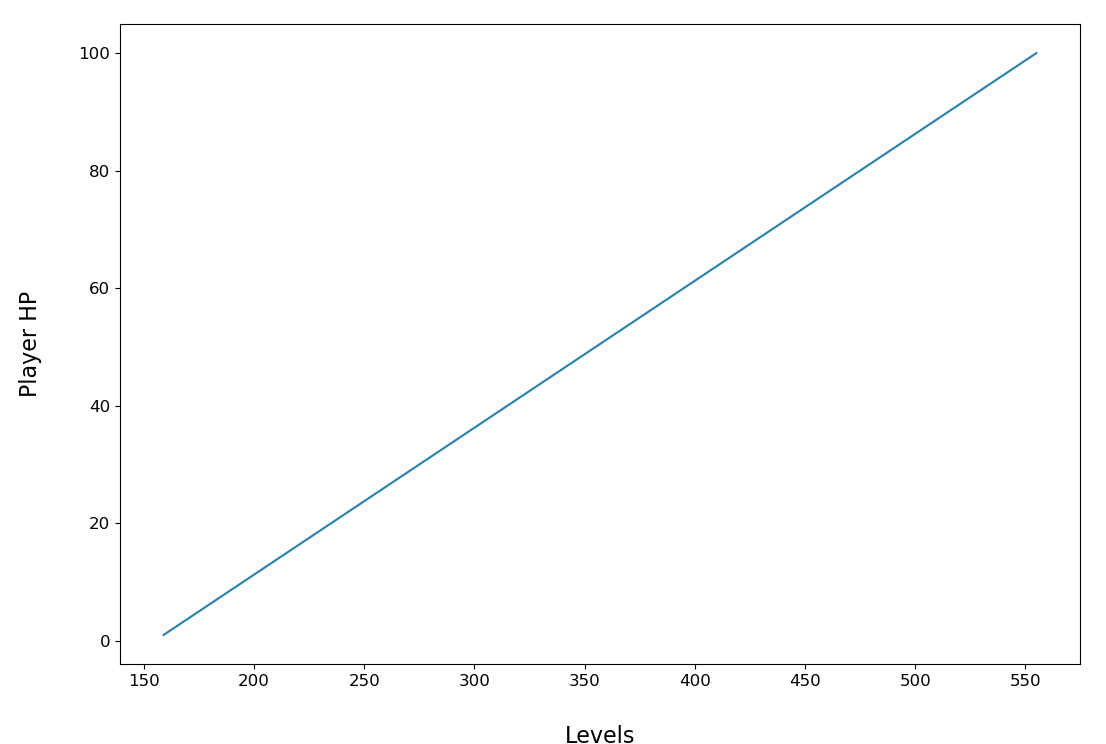
\includegraphics[scale=0.5]{img/PlayerHpDistrib.png}
	\caption{Kenaikan HP setiap levelnya.}
	\vspace{1ex}
	\label{fig:hp_player}
\end{figure}
\vspace{3ex}

\begin{figure} [!h] \centering
	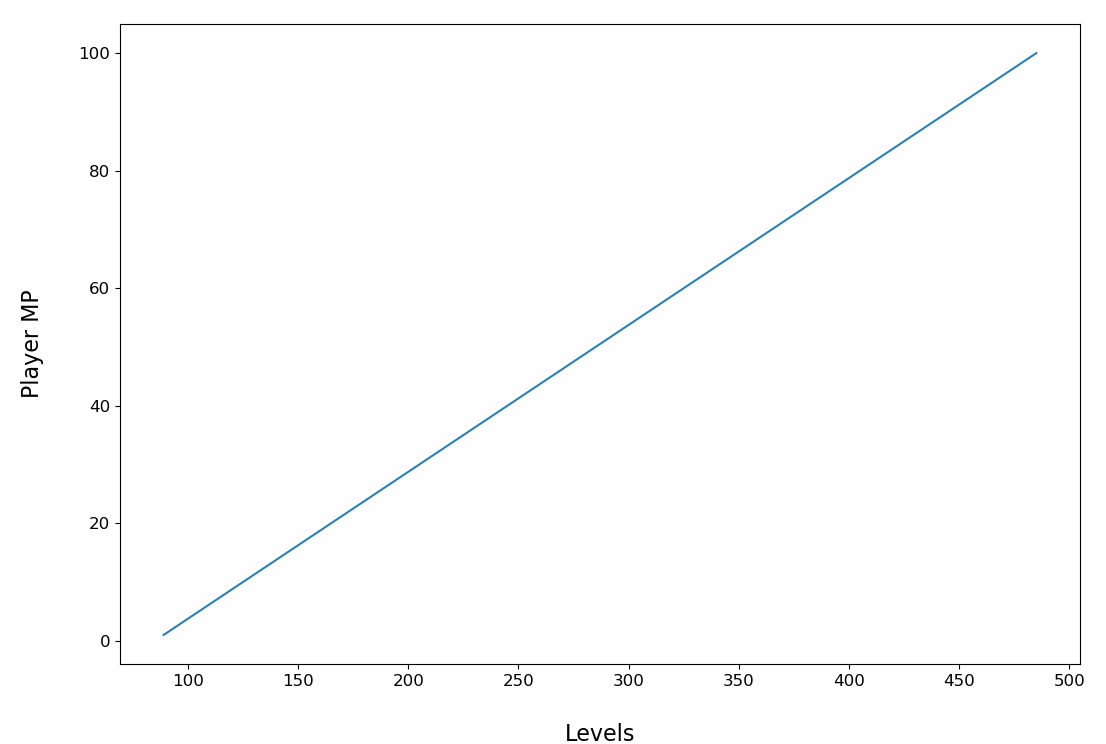
\includegraphics[scale=0.5]{img/PlayerMpDistrib.png}
	\caption{Kenaikan MP setiap levelnya.}
	\label{fig:mp_player}
\end{figure}

Jika melihat Gambar \ref{fig:hp_player} dengan jumlah HP dari pemain yang terus naik mengikuti pola yang dihasilkan pada Tabel \ref{tb:player_hp_mp}, yang mana nilai tersebut diperoleh dari inisiasi variabel pada Tabel \ref{tb:player_input_variable} yaitu \textit{Max Level}, \textit{Start} HP dan \textit{Next} HP. Variabel-variabel tersebut dihitung dengan menggunakan persamaan \ref{eq:hp_player} agar membentuk pola kenaikan HP setiap levelnya seperti yang ditunjukan pada Gambar \ref{fig:hp_player}.
\vspace{1ex}

Sama seperti pada Gambar \ref{fig:hp_player}, pada Gambar \ref{fig:mp_player} dengan jumlah MP dari pemain yang terus naik mengikuti pola yang dihasilkan pada Tabel \ref{tb:player_hp_mp}, yang mana nilai tersebut diperoleh dari inisiasi variabel pada Tabel \ref{tb:player_input_variable} yaitu \textit{Max Level}, \textit{Start} MP dan \textit{Next} MP. Kemudian variabel-variabel tersebut dihitung dengan menggunakan persamaan \ref{eq:mp_player} agar membentuk pola kenaikan MP setiap levelnya seperti yang ditunjukan pada Gambar \ref{fig:mp_player}.
\vspace{1ex}

\subsection{Distribusi Elemen dan Kelemahan Pemain}
\label{sec:sub_sec3_list_element_player}
\vspace{1ex}

Kemudian untuk variabel \textit{List Element} berisi elemen apa saja yang akan diterapkan pada permainan tersebut, seperti yang ditunjukan oleh Tabel \ref{tb:player_input_variable}. Yang mana maksud dari variabel ini adalah memberi penjelasan dari kelemahan dan keunggulan dari pemain berdasarkan elemen, seperti yang sudah dijelasakan pada Sub-bab \ref{sec:sub_sec3_design_skenario} tentang elemen dan efektifitas serangan. Di lanjutkan dengan variabel \textit{List Weaknesses} yang memuat angka-angka yang bertujuan menggambarkan saat pemain menerima serangan dari lawan, berikut adalah penjelasan dari angka-angka tersebut.

\begin{enumerate}[label=\alph*).]
	\item \textbf{Angka 0} adalah \textit{Normal} atau efek serangan bersifat normal tanpa tambahan bonus serangan dan lain sebagainya.
	
	\item \textbf{Angka 1} adalah \textit{Repel} atau memiliki sifat menghindari serangan atau bahkan menghindari serangan.
	
	\item \textbf{Angka 2} adalah \textit{Weaknesess} atau serangan tepat menyerang terhadap kelemahan dari pemain sehingga efek kerusakan atau \textit{damage} menjadi lebih terasa, biasanya dua kali serangan normal.
\end{enumerate}

Pembagian elemen pada pemain bersifat pada penelitian ini dibuat statis, maksudnya elemen yang dari awal didefinisikan tidak akan berubah sampai akhir level, untuk kedepannya hal seperti inilah yang akan menjadi konsetrasi pengembangan program ini berikut juga desainer permainan. Cukup dengan melakukan \textit{override} maka diperolehlah fungsi baru yang bisa menghasilkan perubahan elemen di level tertentu.
\vspace{1ex}

Pada bagian selanjutnya adalah pembahasan mengenai pembagian \textit{stats} jika merujuk pada Tabel \ref{tb:player_input_variable} dengan variabel \textit{List Stats Name} yang berisi nama atau info \textit{stats} dari pemain yang akan digunakan. Kemudian diikuti dengan variabel \textit{Max Stats Value} yang berisi nilai maksimum \textit{stats} yang akan dihasilkan. Lebih detailnya untuk bagian ini, akan dibahas secara khusus pada bagian tersendiri yaitu pada Sub-bab \ref{sec:sub_sec3_stat_pemain}.
\vspace{1ex}

\subsection{Distribusi Stats Pemain}
\label{sec:sub_sec3_stat_pemain}
\vspace{1ex}

Pada bagian ini akan dibahas tentang pembagian \textit{stats} dengan beracuan pada Tabel \ref{tb:player_input_variable} dengan variabel \textit{List Stats Name} yang berisi nama atau info \textit{stats} dari pemain yang akan digunakan. Kemudian diikuti dengan variabel \textit{Max Stats Value} yang berisi nilai maksimum \textit{stats} yang akan dihasilkan. Pada tahap ini digunakannya metode $k-$Nearest Neighbor ($k-$NN) seperti yang sudah dijelaskan pada Sub-bab \ref{sec:sub_sec2_knn} dan Naive Bayes yang juga sudah dijelaskan pada Sub-bab \ref{sec:sub_sec2_bayes}. Pada persamaan \ref{eq:KNN_distance_metrics} yang kemudian disesuaikan dengan pertambahan nilai \textit{Stats to Assign} dari Tabel \ref{tb:player_input_variable}, yang mana nilai tersebut ditambahkan secara acak antara 2 dan 1 dengan perhitungan \textit{class probability} pada persamaan \ref{eq:nbayes_class} yang disesuaikan menjadi persamaan \ref{eq:nbayes_class_stats}. Hasil proses acak tersebut juga harus dibatasi jumlahnya dengan persamaan \ref{eq:KNN_distance_stats}. Maka hasil dari proses acak pada persamaan tersebut akan sangat menentukan perhitungan dari persamaan \ref{eq:KNN_bayes_player_stats}.

\begin{equation}\label{eq:nbayes_class_stats}
\begin{split}
P(C_{St = 1}) = \frac{C_{St = 1}}{(C_{St = 1}\ +\ C_{St = 2})} \\
P(C_{St = 2}) = \frac{C_{St = 2}}{(C_{St = 1}\ +\ C_{St = 2})}
\end{split}
\end{equation}

\begin{equation}\label{eq:KNN_distance_stats}
\begin{split}
D(x,\ p) = \sqrt{(x - p)^2}
\end{split}
\end{equation}

\begin{equation}\label{eq:KNN_bayes_player_stats}
\begin{split}
MaxSt = \left\{\begin{matrix}
\sum_{n = 0}^{N}\ St_{(n)}, & saat\ D(x,\ p) \geqslant 2,\ St = 2 \\ 
\sum_{n = 0}^{N}\ St_{(n)}, & saat\ D(x,\ p) \geqslant 1,\ St = 1 \\
\hspace{4.5em} 0, 			& \hspace{-7.8em} lainnya
\end{matrix}\right.
\end{split}
\end{equation}

Pada persamaan \ref{eq:nbayes_class}, variabel $P(C_{St = 1})$ adalah probabilitas munculnya \textit{Stats To Assign} ke 1 dan $P(C_{St = 2})$ adalah probabilitas munculnya \textit{Stats To Assign} ke 2, kemudian $C_{St = 1}$ adalah jumlah angka satu dan $C_{St = 2}$ adalah jumlah angka satu pada \textit{Stats To Assign}. Setiap stats hasil pengacakan tentunya juga akan dibatasi jumlahnya dengan melakukan \textit{checking} pada maksimum stats, hal tersebut dijelaskan pada persamaan \ref{eq:KNN_distance_stats} yang mana $x$ adalah maksimum stats, $D$ adalah maksimum stats dan $p$ adalah stats saat ini. Kemudian nilai $MaxSt$ pada persamaan \ref{eq:KNN_bayes_player_stats} adalah nilai maksimum stats yang ingin dicapai dengan jumlah $St_{(n)}$ yang dihitung melalui proses pada persamaan \ref{eq:KNN_distance_stats} dan \ref{eq:nbayes_class_stats}.

\begin{equation}\label{eq:nbayes_class_stats_1}
\begin{split}
P(C_{St = n}) = \frac{C_{St = n}}{(C_{St = 0}\ +\ C_{St = 1} +\ C_{St = n})}
\end{split}
\end{equation}

\begin{equation}\label{eq:KNN_distance_stats_1}
\begin{split}
D(x,\ p) = \sqrt{(x - p)^2}
\end{split}
\end{equation}

\begin{equation}\label{eq:KNN_bayes_player_stats_1}
\begin{split}
MaxSt = \left\{\begin{matrix}
\sum_{n = 0}^{N}\ St_{(n)}, & saat\ D(x,\ p) \geqslant n_{st},\ St = n_{st} \\
\sum_{n = 0}^{N}\ St_{(n)}, & \hspace{-1.5em}saat\ D(x,\ p) \geqslant 2,\ St = 2 \\
\sum_{n = 0}^{N}\ St_{(n)}, & \hspace{-1.5em}saat\ D(x,\ p) \geqslant 1,\ St = 1 \\
\hspace{4.5em} 0, 			& \hspace{-9.3em} lainnya
\end{matrix}\right.
\end{split}
\end{equation}

Sedangakan pada persamaan \ref{eq:nbayes_class_stats_1}, \ref{eq:KNN_distance_stats_1} dan \ref{eq:KNN_bayes_player_stats_1} digunakan saat jumlah atau dimensi \textit{Stats to Assign} lebih dari 2. Selanjutnya melalui persamaan \ref{eq:KNN_bayes_player_stats} dan beberapa persamaan yang digunakan sebelumnya dihasilkan data seperti yang ditunjukan pada Tabel \ref{tb:player_battle_stats}, dan bila divisualisasikan hasilnya akan tampak seperti pada Gambar \ref{fig:stats_player}.
\vspace{1ex}

\begin{table}[!h]
	\centering
	\caption{Sampel hasil perhitungan dan distribusi stats dengan $k-$NN}
	\label{tb:player_battle_stats}
	\begin{tabular}{|l|l|l|l|l|l|}
		\hline
		\rowcolor[HTML]{C0C0C0} 
		\textbf{Levels} & \textbf{Strength} & \textbf{Magic} & \textbf{Endurance} & \textbf{Speed} & \textbf{Luck} \\ \hline
		1 & 1 & 2 & 0 & 0 & 1 \\ \hline
		2 & 0 & 2 & 0 & 2 & 0 \\ \hline
		3 & 1 & 0 & 0 & 0 & 0 \\ \hline
		4 & 1 & 1 & 0 & 0 & 0 \\ \hline
		5 & 1 & 1 & 0 & 0 & 0 \\ \hline
		6 & 1 & 1 & 0 & 2 & 1 \\ \hline
		7 & 0 & 0 & 0 & 0 & 1 \\ \hline
		8 & 1 & 0 & 0 & 0 & 0 \\ \hline
		... & ... & ... & ... & ... & ... \\ \hline
		\textbf{100} & \textbf{1} & \textbf{0} & \textbf{0} & \textbf{0} & \textbf{0} \\ \hline
	\end{tabular}
\end{table}
\vspace{1ex}

Pada Tabel \ref{tb:player_battle_stats} adalah data \textit{stats} dari pemain yang dihasilakn melalui penambahan nilai pada \textit{stats} secara acak pada setiap \textit{stats}. Seperti yang dijelaskan pada persaamaan \ref{eq:nbayes_class}, \ref{eq:KNN_distance_stats}, dan persamaan \ref{eq:KNN_bayes_player_stats} saat nilai \textit{stats} di tambahkan secara acak dari 1 sampai dengan 2 pada level yang berjarak antara 1 sampai dengan 100. Selanjutnya representasi dari hasil penambahan \textit{stats} tersebut yang ditunjukan melalui Gambar \ref{fig:stats_player} yang mana nilai dari setiap \textit{stats} terus naik sesuai dengan level pemain yang juga terus naik. 
\vspace{1ex}

\begin{figure} [!h] \centering
	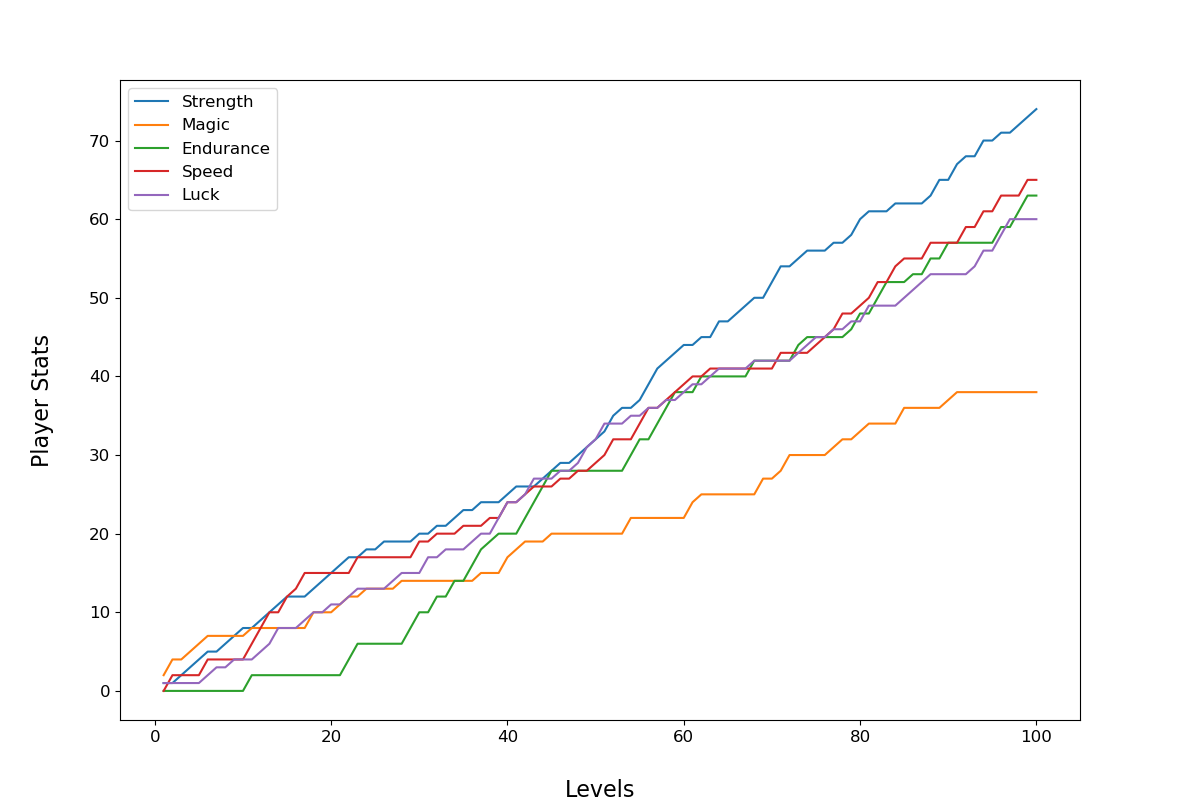
\includegraphics[scale=0.5]{img/PlayerStatsDistrib.png}
	\caption{Kenaikan stats pemain setiap levelnya.}
	\label{fig:stats_player}
\end{figure}
\vspace{1ex}

\section{Desain Level dan Stats pada Karakter Musuh}
\label{sec:sec3_enemy_stats}
\vspace{1ex}

Sama halnya dengan karakter pemain maka dibuatlah sebuah program yang secara otomatis dapat membuat \textit{stats} musuh dengan masukan sesuai dengan kebutuhan desainer permainan atau developer. Program tersebut terdiri dari beberapa fungsi yang pada awalnya adalah obyek yang memiliki masukan parameter-parameter yang nantinya akan menghasilkan sebuah data yang berupa \textit{stats} dari karakter pemain seperti proses yang ditunjukan oleh diagram alur sederhana pada Gambar \ref{fig:enemy_stats_generator}.
\vspace{1ex}

\begin{figure} [!h] \centering
	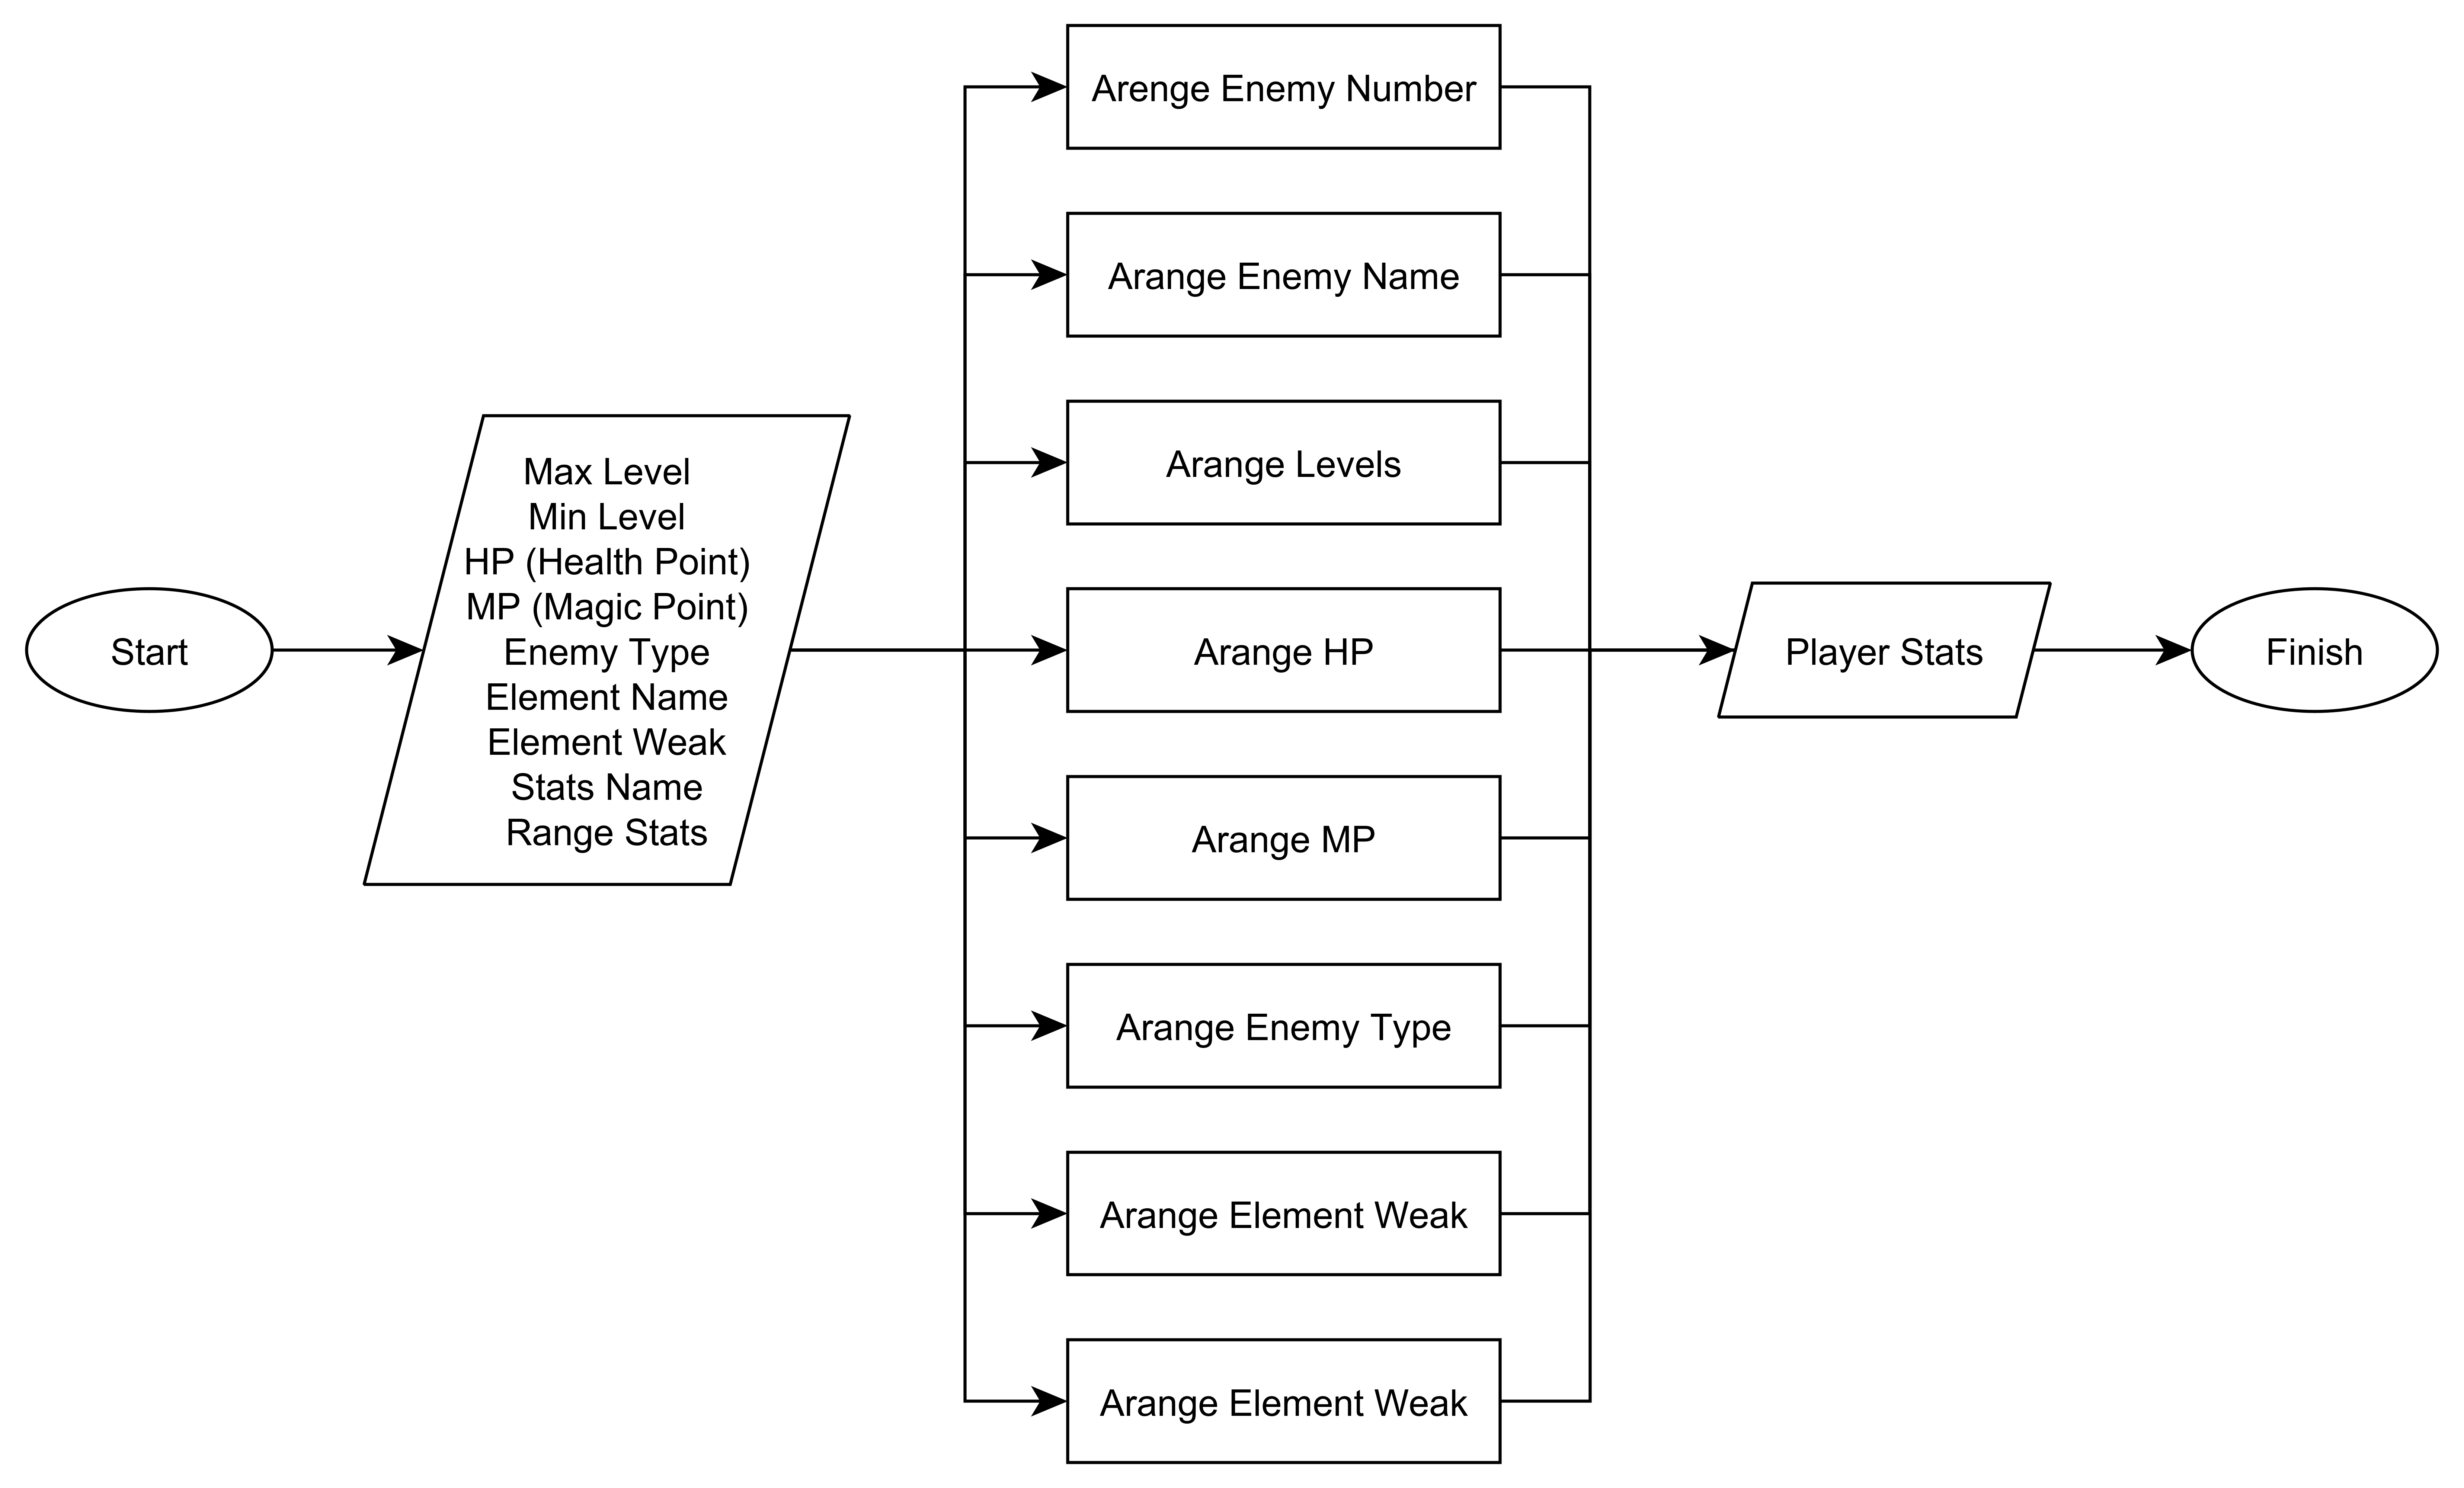
\includegraphics[scale=0.06]{img/enemy_stats_generator.png}
	\caption{Proses pembuatan stats untuk karakter musuh.}
	\label{fig:enemy_stats_generator}
\end{figure}

Pada permainan dengan genre \textit{turn-based} RPG dengan jumlah yang sangat banyak dan beragam, maka program yang ditunjukan melalui proses pada Gambar \ref{fig:enemy_stats_generator} dapat dijalankan satu kali saja, dan menghasilkan banyak musuh. Kecuali ingin menghasilkan kombinasi musuh yang berbeda, misalnya pada proses \textit{generate} yang pertama menghasilkan musuh yang memiliki kemampuan \textit{magic} dan kelemahan sedangkan pada kombinasi musuh selanjutnya tidak memiliki kemampuan \textit{magic}, hanya mengandalkan kemampuan fisik saja. Sama halnya dengan permainan \textit{action} RPG saat proses pembuatan stats musuh.
\vspace{1ex}

Pada Gambar \ref{fig:enemy_stats_generator} di sisi masukan program terdapat banyak sekali masukan variabel seperti \textit{Max Level} yang berupa maksimum level yang diinginkan, kemudian \textit{Min Level} yang berupa minimum level dari musuh, kemudian HP yang berupa \textit{range} atau jarak antara HP minimum dengan HP tertinggi. Sama halnya dengan HP, dalam perhitungan \textit{range} atau jarak, pada \textit{MP} juga menggunakan perhitungan dengan cara tersebut. Kemudian \textit{Enemy Type} yang berisi klasifikasi jenis stats musuh, tergolong musuh seperti apakah stats yang dihasilkan tersebut. Selanjutnya adalah \textit{Element Name} yang berisi daftar elemen apa saja yang dapat dipilih saat pembuatan karakter musuh, selanjutnya \textit{Element Weak} berisi tetang kelemahan dan keunggulan dari musuh tersebut ketika diserang, apakah saat diserang dengan menggunakan elemen tersebut akan mengalami kerusakan atau damage yang parah, normal atau tidak mempan sama sekali. Kemudian untuk \textit{Stats Name} berisikan nama \textit{stats} yang dipakai dalam membuat karakter musuh. Selanjutnya adalah isi atau data dari \textit{stats} itu sendiri yang menentukan karakter dari musuh itu sendiri, seberapa kuat musuh tersebut dalam menyerang atau bertahan dan lain sebagainya. Lebih detail tentang program yang dibuat dapat dilihat pada Gambar \ref{fig:enemy_uml}, yang merupakan \textit{class} diagram untuk membuat \textit{stats} pemain.
\vspace{1ex}

\begin{figure} [!h] \centering
	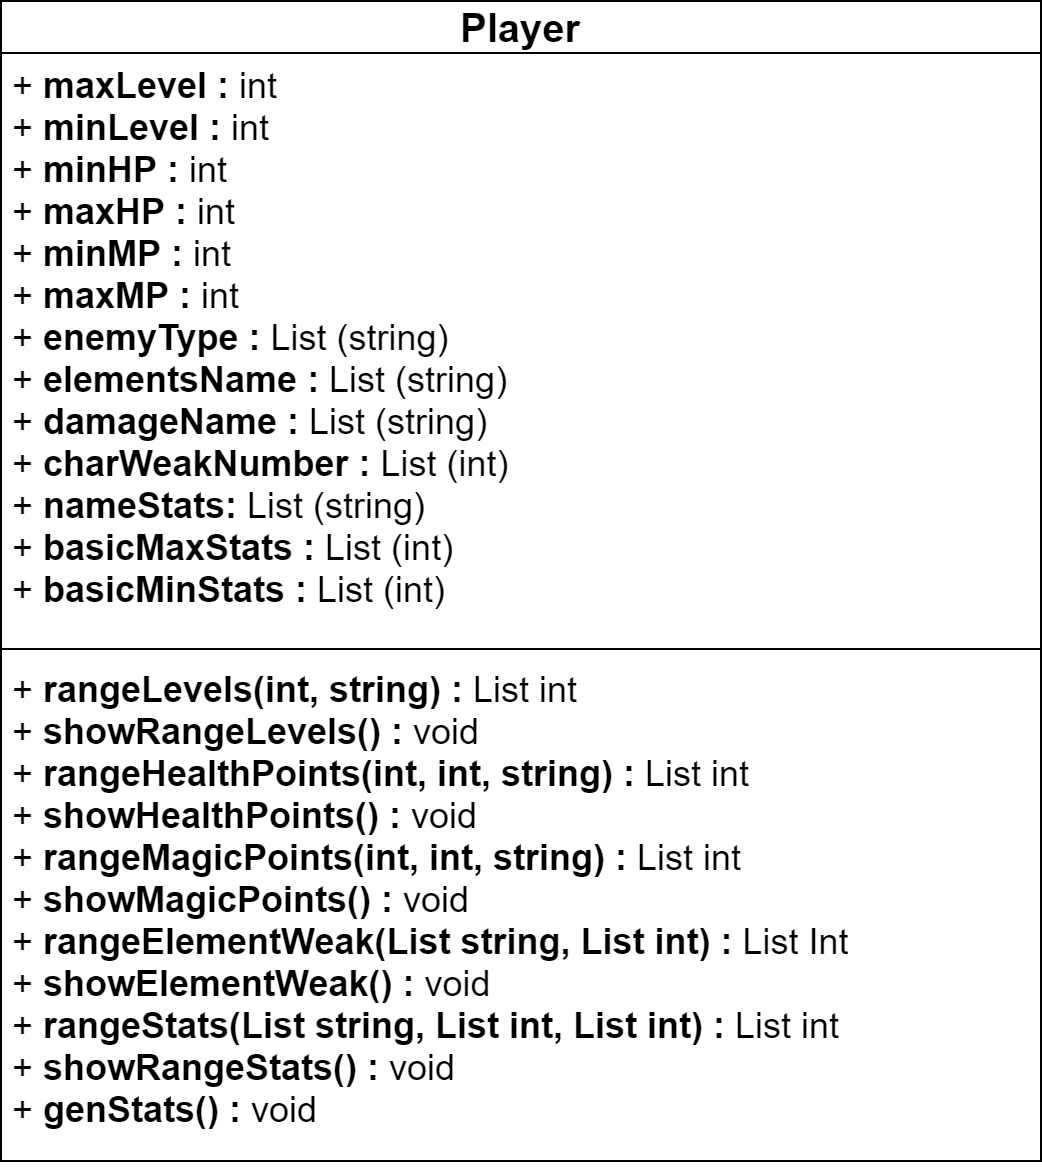
\includegraphics[scale=0.25]{img/enemy_uml.png}
	\caption{\textit{Class} diagram untuk \textit{stats} musuh.}
	\label{fig:enemy_uml}
	\vspace{-1ex}
\end{figure}

Karena program ini dibangun menggunakan OOP (\textit{Object Oriented Programming}) maka program ini dapat dijabarkan menggunakan Gambar \ref{fig:enemy_uml}. Selain itu program ini juga dapat secara mudah dimodifikasi untuk keperluan pengembangan kedepannya, dengan fungsi-fungsi yang ada sangat memungkinkan dilakukan \textit{override} atau pembuatan fungsi yang sama dengan isi atau proses yang berbeda seperti pada penjelasan dibagian pemain pada Sub-bab \ref{sec:sec3_player_stats}. Seperti pada bagian sebelumnya maka dibuatlah Tabel \ref{tb:enemy_input_variable} yang berupa masukan untuk menguji program yang akan dijelaskan pada bagian-bagian selanjutnya, yang mana masukan pada tabel tersebut akan menghasilkan stats pada sebuah karakter untuk pemain.
\vspace{1ex}

\begin{table}[!h]
	\centering
	\caption{Data masukan untuk pembuatan program pada musuh.}
	\label{tb:enemy_input_variable}
	\begin{tabular}{|l|l|}
		\hline
		\rowcolor[HTML]{9B9B9B} 
		\multicolumn{1}{|c|}{\cellcolor[HTML]{9B9B9B}\textbf{Variabel}} & \multicolumn{1}{c|}{\cellcolor[HTML]{9B9B9B}\textbf{Input}} \\ \hline
		\textit{Enemy Numbers} & 400 \\ \hline
		\textit{Max Level} & 80 \\ \hline
		\textit{Min Level} & 1 \\ \hline
		\textit{Level Class} & {[} `\textit{Easy}', `\textit{Medium}', `\textit{High}' {]} \\ \hline
		\textit{Min} HP & 159 \\ \hline
		\textit{Max} HP & 163 \\ \hline
		\textit{Min} MP & 89 \\ \hline
		\textit{Max} MP & 93 \\ \hline
		\textit{Enemy Type} & \begin{tabular}[c]{@{}l@{}}{[} `\textit{Mixed}', `\textit{Hard Magic}', `\textit{Soft Magic}', \\ \ \ `\textit{Hard Strength}', `\textit{Soft Magic}' {]}\end{tabular} \\ \hline
		\textit{Distribution Percentage} & {[} 40, 10, 20, 10, 20 {]} \\ \hline
		\textit{List Element} & {[} `\textit{Phys}', `\textit{Water}', `\textit{Wind}', `\textit{Earth}', `\textit{Fire}' {]} \\ \hline
		\textit{List Damage} & {[} `\textit{Normal}', `\textit{Repel}', `\textit{Weak}' {]} \\ \hline
		\textit{List Stats Name} & \begin{tabular}[c]{@{}l@{}}{[} `\textit{Strength}', `\textit{Magic}', `\textit{Endurance}',\\ \ \ `\textit{Speed}', `\textit{Luck}' {]}\end{tabular} \\ \hline
		\textit{Max Stats Value} & {[} 50, 60, 40, 55, 45 {]} \\ \hline
		\textit{Min Stats Value} & {[} 2, 2, 2, 2, 2 {]} \\ \hline
	\end{tabular}
\end{table}

\subsection{Distribusi Level Musuh}
\label{sec:sub_sec3_enemy_level}
\vspace{1ex}

Pada bagian ini akan dijelaskan tentang pembagian level pada musuh, dengan masukan seperti yang disebutkan pada Tabel \ref{tb:enemy_input_variable}. Beracuan pada tabel tersebut beberapa variabel utama yang akan digunakan diantaranya adalah ``\textit{Enemy Numbers}" yang menentukan jumlah musuh yang akan dibuat, ``\textit{Max Level}" dan ``\textit{Min Level}" adalah nilai maksimum dan minimum level dari musuh yang ingin dibuat. Selanjutnya tingkat kesulitan dari musuh juga ditentukan disini, dengan variabel ``\textit{Level Class}" yang isinya dibagi menjadi ``\textit{Easy}", ``\textit{Medium}" dan ``\textit{Hard}". Musuh dengan \textit{``Level Class"} atau tingkat kesulitan \textit{``Easy"} akan menjadi yang paling mudah dikalahkan, diikuti daengan tingkat kesulitan \textit{``Medium"} dan ``\textit{Hard}" secara berurutan.
\vspace{1ex}

Kemudian terdapat variabel pendukung yang akan menentukan data atau level yang ingin dihasilkan, yaitu \textit{scale}. Selaanjutnya dilakukan beberapa proses seperti pada persamaan \ref{eq:enemy_levels1}, \ref{eq:enemy_levels2}, \ref{eq:sub_enemy_levels1}, dan persamaan \ref{eq:sub_enemy_levels2} yang kemudian diperoleh hasil berupa level untuk banyak musuh sekaligus seperti yang ditunjukan pada persamaan \ref{eq:probability_enemy_levels}.
\vspace{1ex}

\begin{equation}\label{eq:enemy_levels1}
	\resizebox{\columnwidth}{!}{%
		$SL_{N} = \left\{\begin{matrix}
		\hspace{0.2em} \sum_{i = 0}^{N}\ \frac{LN}{LC_{N}} & Saat\ 0 \equiv LN\ (mod\ LC_{N}) & \\
		
		\hspace{0.2em} \sum_{i = 0}^{N}\ \frac{LN}{LC_{N}} & Saat\ 0 \not\equiv LN\ (mod\ LC_{N}), & \\
		&\hspace{1.0em}  0 \not\equiv LC_{N}\ (mod\ 2) & \hspace{-3.5em} \Rightarrow\ SL_{(\left \lceil N/2 \right \rceil)}  = \left \lceil \frac{LN}{LC_{N}} \right \rceil &\\
		
		& & \hspace{-6.0em} \Rightarrow\ SL_{i}  = \left \lfloor \frac{LN}{LC_{N}} \right \rfloor &\\
		
		\hspace{0.2em} \sum_{i = 0}^{N}\ \frac{LN}{LC_{N}} & Saat\ 0 \not\equiv LN\ (mod\ LC_{N}), & \\
		&\hspace{1.0em}  0 \equiv LC_{N}\ (mod\ 2) & \Rightarrow\ SL_{N/2},\ SL_{(N/2) + 1}  = \left \lceil \frac{LN}{LC_{N}} \right \rceil &\\
		
		& & \hspace{-6.0em} \Rightarrow\ SL_{i}  = \left \lfloor \frac{LN}{LC_{N}} \right \rfloor &\\
		\end{matrix}\right.$%
	}
\end{equation}
\vspace{1ex}

Pada persamaan \ref{eq:enemy_levels1} adalah proses pembagian dari jumlah level dari musuh yang dijelaskan pada Tabel \ref{tb:enemy_input_variable} pada variabel \textit{Max Level} dan \textit{Min Level} sebagai \textit{range} yang merupakan level dari musuh yang disimbolkan dengan $LN$ yang kemudian dibagi dengan  $LC_{N}$ yang merupakan jumlah kelompok atau \textit{cluster} data dari \textit{level class}. Jika beracuan pada Tabel \ref{tb:enemy_input_variable} maka jumlah \textit{cluster} level adalah jumlah data atau level yang dimuat pada setiap variabel didalam ``\textit{Level Class}" seperti ``\textit{Easy}", ``\textit{Medium}" dan ``\textit{High}", jadi jumlah levelnya adalah 3 \textit{cluster} level. Jadi pada kasus yang dicontohkan ini $LC = \left \{1, 2, 3 \right \}$, kemudian jika jumlah \textit{cluster} level ingin dibuat lebih dari contoh maka $LC = \left \{1, 2, 3,..., LC_{N} \right \}$ dengan $N$ adalah jumlah \textit{cluster} level yang ingin dibuat.
\vspace{1ex}

Dalam proses pencarian $SL_{N}$ atau \textit{cluster} level yang terbagi menjadi tiga tersebut, terdapat beberapa keputusan yang harus dijalankan. Seperti hanya hasil bagi antara $LN$ dan $LC_{N}$ harus bernilai bilangan tidak bulat, maka harus dilakukan proses pembulatan jumlah level terlebih dahulu dikarenakan nilai level tidak boleh bernilai angka yang tidak bulat. Sepeti pada persamaan \ref{eq:enemy_levels1} untuk dilakukan pengujian apakah dapat dibulatkan maka dilakukan operasi modulus atau $mod$, jika habis maka $SL_{N}$ akan diisi secara merata oleh hasil bagi antara $LN$ dan $LC_{N}$. Maka jumlah \textit{cluster} sebanyak $N$ pada $LC_{N}$ dan banyaknya level adalah sebesar $LN$ yang dibagi dengan $LC_{N}$ yang kemudian hasil akhir tersebut disimpan dalam variabel $SL_{N}$. 
\vspace{1ex}

Namun jika tidak dapat dibagi secara merata maka dilakukan terlebih dahulu proses pengecekkan apakah jumlah $LC_{N}$ apakah berjumlah ganjil atau genap, hal tersebut dilakukan dengan cara melakukan modulus dari $LC_{N}$ dengan angka 2. Jika ternyata $LC_{N}$ bernilai genap maka $SL_{N}$ atau jumlah \textit{cluster} akan dibagi menjadi dua bagian, kemudian dua nilai tengah setelah dibagi menjadi dua bagian tersebut diisi dengan jumlah level yang lebih tinggi jika dibandingkan dengan \textit{cluster} level yang lain. Kemudian jika $LC_{N}$ bernilai ganjil maka nilai tengah dari jumlah \textit{cluster} tersebutlah yang akan memiliki jumlah level lebih banyak jika dibandingkan dengan \textit{cluster} level yang lain.
\vspace{1ex}

\begin{equation}\label{eq:enemy_levels2}
\resizebox{\columnwidth}{!}{%
	$SE_{N} = \left\{\begin{matrix}
	\hspace{0.2em} \sum_{i = 0}^{N}\ \frac{EN}{LC_{N}} & Saat\ 0 \equiv EN\ (mod\ LC_{N}) & \\
	
	\hspace{0.2em} \sum_{i = 0}^{N}\ \frac{EN}{LC_{N}} & Saat\ 0 \not\equiv EN\ (mod\ LC_{N}), & \\
	&\hspace{1.0em}  0 \not\equiv LC_{N}\ (mod\ 2) & \hspace{-4.0em} \Rightarrow\ SE_{(\left \lceil N/2 \right \rceil)}  = \left \lceil \frac{EN}{LC_{N}} \right \rceil &\\
	
	& & \hspace{-6.2em} \Rightarrow\ SE_{i}  = \left \lfloor \frac{EN}{LC_{N}} \right \rfloor &\\
	
	\hspace{0.2em} \sum_{i = 0}^{N}\ \frac{EN}{LC_{N}} & Saat\ 0 \not\equiv EN\ (mod\ LC_{N}), & \\
	&\hspace{1.0em}  0 \equiv LC_{N}\ (mod\ 2) & \Rightarrow\ SE_{N/2},\ SE_{(N/2) + 1}  = \left \lceil \frac{EN}{LC_{N}} \right \rceil &\\
	
	& & \hspace{-6.2em} \Rightarrow\ SE_{i}  = \left \lfloor \frac{EN}{LC_{N}} \right \rfloor &\\
	\end{matrix}\right.$%
}
\end{equation}
\vspace{1ex}

Munculah pertanyaan berapakah jumlah level pada dua \textit{cluster} level tengah pada kasus $LC_{N}$ dengan nilai genap, dan berapakah jumlah level pada \textit{cluster} level pada bagian tengah untuk kasus $LC_{N}$ dengan nilai ganjil. Seperti pada persamaan \ref{eq:enemy_levels1} jika pada kondisi genap maka dua \textit{cluster} level bagian tengah diisi dengan level sejumlah hasil pembagian $LN$ dengan $LC_{N}$ yang dibulatkan ke atas atau \textit{ceil}, sedangkan pada kondisi ganjil maka 1 \textit{cluster} level bagian tengahlah yang diisi dengan hasil pembagian tersebut. Kemudian untuk jumlah level pada \textit{cluster} yang lain diisi dengan pembagian $LN$ dengan $LC_{N}$ yang dibulatkan ke bawah atau \textit{floor}. Jika $SL_{N}$ adalah jumlah \textit{cluster} level, maka perlu dicari juga jumlah cluster untuk musuh dengan menggunakan persamaan \ref{eq:enemy_levels2} dengan cara yang sama dengan pencarian jumlah \textit{cluster} level. 
\vspace{1ex}

Dalam proses pencarian $SE_{N}$ atau \textit{cluster} musuh pada persamaan \ref{eq:enemy_levels2} digunakan cara yang sama seperti cara perhitungan pada persamaan \ref{eq:enemy_levels1} dengan membagi jumlah musuh ke dalam tiga bagian, dan dilanjutkan dengan pengambilan beberapa keputusan yang harus dijalankan. Sama seperti pada perhitungan hasil bagi antara $LN$ dan $LC_{N}$ pada persamaan \ref{eq:enemy_levels1}, nilai pembagian $EN$ atau jumlah musuh yang ingin dihasilkan dengan $LC_{N}$ atau jumlah \textit{cluster} musuh yang ingin dibuat dengan tiga tingkatan ``\textit{Easy}", ``\textit{Medium}" dan ``\textit{Hard}" yang juga harus bernilai bilangan bulat positif, kemudian dilakukan juga proses pembulatan jumlah musuh terlebih dahulu dikarenakan jumlah musuh tidak boleh bernilai angka yang tidak bulat. 
\vspace{1ex}

Sepeti pada persamaan \ref{eq:enemy_levels1} pada persamaan \ref{eq:enemy_levels2} juga dilakukan pengujian apakah dapat dibulatkan atau tidak maka dilakukan operasi modulus atau $mod$, jika habis maka $SE_{N}$ akan diisi secara merata oleh hasil bagi antara $EN$ dan $LC_{N}$. Maka jumlah \textit{cluster} sebanyak $N$ pada $LC_{N}$ dan banyaknya musuh adalah sebesar $EN$ yang dibagi dengan $LC_{N}$, kemudian hasil akhir tersebut disimpan dalam variabel $SE_{N}$. Untuk penjelasan langkah selanjutnya pada persamaan \ref{eq:enemy_levels2} sama persis dengan persamaan \ref{eq:enemy_levels1} yang sudah dijelaskan pada bagian sebelumnya, hanya saja objek pada persamaan \ref{eq:enemy_levels1} adalah level sedangkan pada persamaan \ref{eq:enemy_levels2} adalah musuh. Setelah $SL_{N}$ dan $SE_{N}$ diperoleh maka saatnya menuju bagian yang lebih dalam dan detail lagi. Bagaimana dengan pemberian level untuk setiap musuh, maka digunakanlah persamaan \ref{eq:sub_enemy_levels1} dan persamaan \ref{eq:sub_enemy_levels2} dengan penjelasan sebagai berikut.
\vspace{1ex}

\begin{equation}\label{eq:sub_enemy_levels1}
\resizebox{\columnwidth}{!}{%
	$SSL_{N} = \left\{\begin{matrix}
	\hspace{0.2em} \sum_{i = 0}^{N}\ \frac{SL}{Sc} & Saat\ 0 \equiv SL\ (mod\ Sc) & \\
	
	\hspace{0.2em} \sum_{i = 0}^{N}\ \frac{SL}{Sc} & Saat\ 0 \not\equiv SL\ (mod\ Sc), & \\
	&\hspace{1.4em}  0 \not\equiv Sc\ (mod\ 2) & \hspace{-4.5em} \Rightarrow\ SSL_{(\left \lceil N/2 \right \rceil)}  = \left \lceil \frac{SL}{Sc} \right \rceil &\\
	
	& & \hspace{-6.8em} \Rightarrow\ SSL_{i}  = \left \lfloor \frac{SL}{Sc} \right \rfloor &\\
	
	\hspace{0.2em} \sum_{i = 0}^{N}\ \frac{SL}{Sc} & Saat\ 0 \not\equiv SL\ (mod\ Sc), & \\
	&\hspace{1.3em}  0 \equiv Sc\ (mod\ 2) & \Rightarrow\ SSL_{N/2},\ SSL_{(N/2) + 1}  = \left \lceil \frac{SL}{Sc} \right \rceil &\\
	
	& & \hspace{-6.7em} \Rightarrow\ SSL_{i}  = \left \lfloor \frac{SL}{Sc} \right \rfloor &\\
	\end{matrix}\right.$%
}
\end{equation}

\begin{equation}\label{eq:sub_enemy_levels2}
\resizebox{\columnwidth}{!}{%
	$SSE_{N} = \left\{\begin{matrix}
	\hspace{0.2em} \sum_{i = 0}^{N}\ \frac{SE}{Sc} & Saat\ 0 \equiv SE\ (mod\ Sc) & \\
	
	\hspace{0.2em} \sum_{i = 0}^{N}\ \frac{SE}{Sc} & Saat\ 0 \hspace{0.3em} \not\equiv SE\ (mod\ Sc), & \\
	&\hspace{1.3em}  0 \not\equiv Sc\ (mod\ 2) & \hspace{-4.5em} \Rightarrow\ SSE_{(\left \lceil N/2 \right \rceil)}  = \left \lceil \frac{SE}{Sc} \right \rceil &\\
	
	& & \hspace{-6.6em} \Rightarrow\ SSE_{i}  = \left \lfloor \frac{SE}{Sc} \right \rfloor &\\
	
	\hspace{0.2em} \sum_{i = 0}^{N}\ \frac{SE}{Sc} & Saat\ 0 \not\equiv SE\ (mod\ Sc), & \\
	&\hspace{1.2em}  0 \equiv Sc\ (mod\ 2) & \Rightarrow\ SSE_{N/2},\ SSE_{(N/2) + 1}  = \left \lceil \frac{SE}{Sc} \right \rceil &\\
	
	& & \hspace{-6.6em} \Rightarrow\ SSE_{i}  = \left \lfloor \frac{SE}{Sc} \right \rfloor &\\
	\end{matrix}\right.$%
}
\end{equation}
\vspace{1ex}

Setelah diperolehnya $SL_{N}$ dan $SE_{N}$ yang masing-masing adalah cluster \textit{level} dan \textit{cluster} musuh, maka dicarilah $SSL_{N}$ atau \textit{sub-cluster} level pada persamaan \ref{eq:sub_enemy_levels1} hal ini betujuan untuk mempersempit \textit{range} dalam pembagian level musuh. Seperti pada penjelasan sebelumnya terdapat satu variabel lagi yang mempengaruhi proses ini, variabel tersebut adalah $SC$ atau skala yang mentukkan kerapatan pembagian level pada setiap musuh. Pada kasus ini $SSL_{N}$ adalah jumlah \textit{sub-cluster} dari setiap level \textit{cluster} atau $SL_{N}$, jadi pada dasarnya persamaan \ref{eq:sub_enemy_levels1} dijalankan setelah nilai $SL_{N}$ diperoleh dan nilai $SSL_{N}$ selalu berubah-ubah mengikuti skala atau \textit{Sc} yang menjadi salah satu masukan untuk fungsi pada program ini. Perhitungan $SSL_{N}$ atau jumlah \textit{sub-cluster} level pada dasarnya sama dengan perhitungan dalam mencari $SL_{N}$ atau $SE_{N}$ pada bagian sebelumnya, hanya saja pada bagian sebelumnya jumlah \textit{cluster} level dan musuh dipengaruhi oleh $LC_{N}$ sedangkan pada $SSL_{N}$ jumlah \textit{sub-cluster} level dipengaruhi oleh $Sc$. Kemudian dilakukan juga pengecekan dengan operasi modulus atau $mod$ antara $SL$ dengan $SC$, apakah $SL$ akan habis jika dibagi dengan $SC$. Jika ternyata $SL$ habis dibagi dengan $Sc$, maka level pada range $SSL$ atau \textit{sub-cluster} tersebut akan langsung dibagi secara merata. Sedangkan pada kondisi sebaliknya yaitu saat $SE$ tidak habis dibagi dengan $Sc$ maka akan dilakukan proses pembulatan ganjil dan genap yang dibulatkan ke atas atau \textit{ceil} seperti pada persamaan \ref{eq:enemy_levels1} dan persamaan \ref{eq:enemy_levels2}, kemudian untuk nilai yang lain dibulatkan ke bawah atau \textit{floor}.
\vspace{1ex}

Kemudian untuk persamaan \ref{eq:sub_enemy_levels2} sama seperti persamaan \ref{eq:sub_enemy_levels2} hanya saja yang menjadi subjek disini adalah $SSE_{N}$ atau \textit{sub-cluster} jumlah musuh. Kemudian cara perhitungannya sama seperti persamaan \ref{eq:sub_enemy_levels1}, yang dibagi adalah \textit{cluster} $SE$ dari musuh dibagi dengan skala atau $Sc$. Saat semua sudah selesai dilakukan, khususnya yang ada pada persamaan \ref{eq:enemy_levels1} dan persamaan \ref{eq:enemy_levels1}. Kemudian dieksekusi setiap \textit{cluster} level dan musuh ke dalam setiap \textit{sub-cluster}, pada setiap \textit{sub-cluster} tersebutlah proses pemberian level pada setiap musuh dilakukan. Pada persamaan \ref{eq:probability_enemy_levels} adalah penjelasan tentang peluang diperolehnya level pada setiap musuh, yang beracuan pada metode \textit{Naive Bayes}, lebih tepatnya lagi adalah tentang peluang marginal.
\vspace{1ex}

\begin{equation}\label{eq:probability_enemy_levels}
\begin{split}
P(Elv_{k}) = \sum_{i = 0}^{M} \sum_{j = 0}^{N} \sum_{k = 0}^{L}\ \frac{Elv_{k}}{Lv_{j} + SSL_{N}}
\end{split}
\end{equation}

Pada persamaan \ref{eq:probability_enemy_levels} $P(Elv_{k})$ adalah peluang munculnya $Elv$ ke $k$, sedangkan $Lv$ ke $j$ adalah batas bawah range level yang dapat diambil oleh musuh. Kemudian $SSL_{N}$ sepeerti yang sudah dijelaskan pada bagian sebelumnya, variabel itu adalah \textit{sub-cluster} dari level. Variabel tersebut dapat digunakan untuk mengubah jarak level saat terjadi perubahan nilai \textit{sub-cluster} yang juga menentukan nilai dari $Elv$ ke $k$. Setelah melalui sekian tahapan yang sudah dijelaskan sebelumnya dan dengan masukan variabeel pada Tabel \ref{tb:enemy_input_variable} maka level yang dihasilkan akan terlihat seperti pada Tabel \ref{tb:enemy_level_distrib}.
\vspace{1ex}

\begin{table}[!h]
	\centering
	\caption{Hasil level yang dibuat untuk musuh.}
	\label{tb:enemy_level_distrib}
	\begin{tabular}{|l|l|l|}
		\hline
		\textbf{No.} & \textbf{Name} & \textbf{Levels} \\ \hline
		1 & Enemy 1 & 1 \\ \hline
		2 & Enemy 2 & 1 \\ \hline
		3 & Enemy 3 & 1 \\ \hline
		4 & Enemy 4 & 1 \\ \hline
		5 & Enemy 5 & 2 \\ \hline
		6 & Enemy 6 & 2 \\ \hline
		7 & Enemy 7 & 2 \\ \hline
		8 & Enemy 8 & 2 \\ \hline
		9 & Enemy 9 & 2 \\ \hline
		10 & Enemy 10 & 2 \\ \hline
		11 & Enemy 11 & 2 \\ \hline
		12 & Enemy 12 & 2 \\ \hline
		13 & Enemy 13 & 2 \\ \hline
		14 & Enemy 14 & 3 \\ \hline
		15 & Enemy 15 & 3 \\ \hline
		... & ... & ... \\ \hline
		\textbf{400} & \textbf{Enemy 400} & \textbf{78} \\ \hline
	\end{tabular}
	\vspace{1ex}
\end{table}


Pada Tabel \ref{tb:enemy_level_distrib} adalah sebagian data dari level yang dihasilkan oleh program, untuk hasil lebih lengkapnya bisa dilihat pada Bagian \nameref{chap:chap6_attachment} pada Tabel \ref{tb:enemies_all_stats_1} sampai dengan Tabel \ref{tb:enemies_all_stats_15} di kolom \textit{Levels}. Kemudian persebaran level yang dihasilkan tersebut bila divisualisasikan maka hasilnya akan seperti yang ditujukkkan pada Gambar \ref{fig:enemy_level_distrib}. Grafik atau histogram yang ditunjukan pada Gambar \ref{fig:enemy_level_distrib} tersebut sangatlah tidak merata, hal tersebut dikarenakan proses penentuan level yang ditentukan secara acak.
\vspace{1ex}

\begin{figure} [!h] \centering
	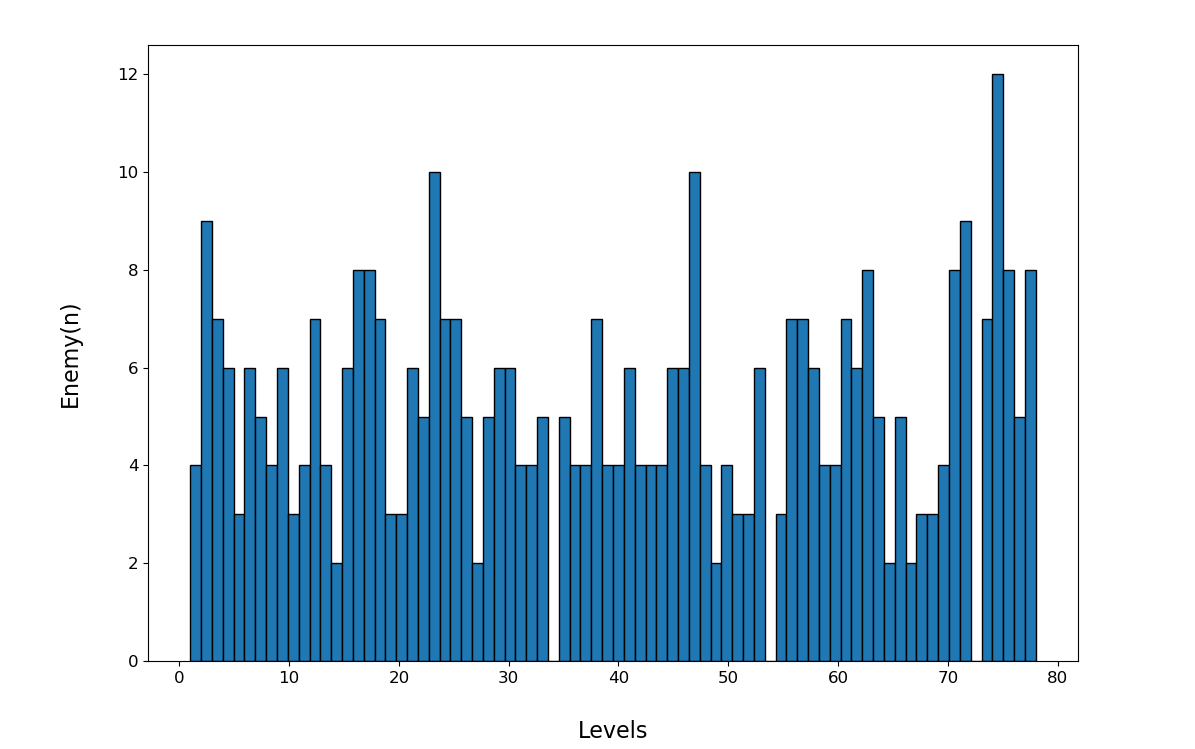
\includegraphics[scale=0.5]{img/EnemyLevelDistrib.png}
	\caption{Distribusi Level Musuh.}
	\label{fig:enemy_level_distrib}
\end{figure}
\vspace{1ex}

Selanjutnya adalah validasi dari keseimbangan persebaran level musuh, hal ini dilakukan dengan menggunakkan persamaan melalui beberapa langkah seperti yang ditunjukan oleh persamaan \ref{eq:mean_enemy_levels}, \ref{eq:varian_enemy_levels}, \ref{eq:stdev_enemy_levels} dan persamaan \ref{eq:PDF_enemy_levels}. Konsep tersebut beracuan pada Sub-bab \ref{sec:sub_sec2_gauss_bayes} tentang \textit{Gaussian Naive bayes}, dengan harapan apakah setiap data yang dihasilkan sebelumnya sudah terdistribusi dengan normal atau tidak. Adapun urutan metode dalam penggunaan \textit{Gaussian Naive Bayes} adalah dengan mencari rata-rata dari data tersebut, kemudian diikuti dengan perhitungan standar deviasi.
\vspace{1ex}

\begin{equation}\label{eq:mean_enemy_levels}
\begin{split}
\bar{E}lv = \frac{\sum_{i = 0}^{N}\ Elv_{i}}{N}
\end{split}
\end{equation}
\vspace{1ex}

Pada persamaan \ref{eq:mean_enemy_levels} adalah rata-rata dari level yang dihasilkan sama seperti pembahasan pada persamaan \ref{eq: mean} yang kemudian disimbolkan dengan variabel $\bar{E}lv$. Selanjutnya adalah $\bar{E}lv_{i}$ adalah setiap level dari musuh yang terus dijumlahkan sebanyak $N$, yang mana $N$ sendiri adalah banyaknya musuh yang sudah dibuat. Setelah diperoleh rata-rata level maka dapat dilanjutkan dengan pencarian nilai \textit{standar deviasi} seperti pada persamaan \ref{eq:stdev_enemy_levels}.
\vspace{1ex}

\begin{equation}\label{eq:varian_enemy_levels}
\begin{split}
\sigma(Elv)^2 = \frac{\sum_{i = 0}^{N}\ (Elv_{i} - \bar{E}lv)^{2}}{N}
\end{split}
\end{equation}

\begin{equation}\label{eq:stdev_enemy_levels}
\begin{split}
\sigma(Elv) = \sqrt{\frac{\sum_{i = 0}^{N}\ (Elv_{i} - \bar{E}lv)^{2}}{N}}
\end{split}
\end{equation}

Pada persamaan \ref{eq:stdev_enemy_levels} adalah persamaan untuk mencari standar deviasi atau $\sigma(Elv)$ setelah diperolehnya rata-rata atau $\bar{E}lv$ melalui persamaan \ref{eq:mean_enemy_levels} yang kemudian dilanjutkan dengan pencarian varian atau $\sigma(Elv)^2$ melalui persamaan \ref{eq:varian_enemy_levels} yang selanjutnya diakar kuadratkan untuk memperoleh nilai standar deviasi. Jika standar deviasi, varian dan rata-rata sudah diperoleh maka dapat dilanjutkan menuju pencarian nilai distribusi normal melalui \textit{Gausian Naive Bayes} seperti pada persamaan \ref{eq:PDF_enemy_levels} berikut ini.
\vspace{1ex}

\begin{equation}\label{eq:PDF_enemy_levels}
\begin{split}
PDF(ELv,\ \bar{E}lv,\ \sigma) = \frac{1}{\sqrt{2 \pi} \sigma}\ exp \left(-\frac{(Elv - \bar{E}lv)^2}{2 \sigma^2}\right)
\end{split}
\end{equation}

Konsep pada persamaan \ref{eq:PDF_enemy_levels} sudah sangat dijelaskan pada Sub-bab \ref{sec:sub_sec2_gauss_bayes} poin ke 3. Hasil perhitungaan sebelumnya yang berupa varian $\sigma^2$, rata-rata $\bar{E}lv$ dan standar deviasi $\sigma$ menjadi masukan pada persamaan tersebut. Variabel $\pi$ adalah konstanta numerik pada umumnya, kemudian fungsi $exp()$ atau $e$ adalah konstanta numerik yang betujuan untuk membentuk hasil prediksi dengan pendekatan exponensial. Jika memang benar data hasil program ini valid maka ketika musuh bertambah maka pola dari level dan jumlah musuh masih akan membentuk pola distribusi normal seperti pada Gambar \ref{fig:enemy_level_distrib_ndist}.

\begin{figure} [!h] \centering
	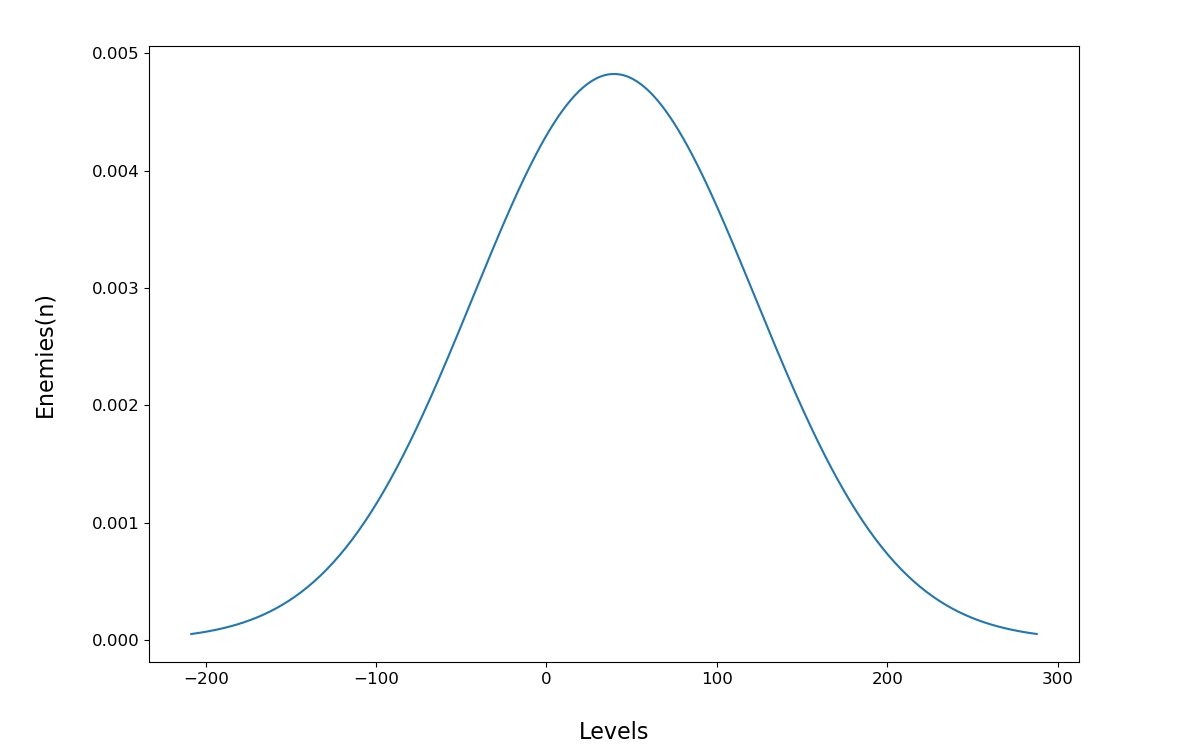
\includegraphics[scale=0.5]{img/EnemyLevelDistribNdist.png}
	\caption{Distribusi level musuh dalam bentuk distribusi normal.}
	\label{fig:enemy_level_distrib_ndist}
\end{figure}

Pada Gambar \ref{fig:enemy_level_distrib_ndist} jika dilihat persebaran datanya dari kiri ke kanan menggambarkan tingkat kesulitan musuh berdasarkan level, jumlah musuh pada sisi kiri berjumlah sedikit semakin ke kanan jumlahnya meningkat dan semakin ke kanan jumlah musuh kembali menjadi sedikit jumlahnya. Hal tersebut menggambarkan tingkat keseimbangan dari musuh yang dibuat, yang mana jumlah musuh dengan level menengah berjumlah paling banyak dan jumlah musuh yang sangat sulit dan sangat mudah dikalahkan berjummlah sedikit. Tujuan utama dari kondisi tersebut adalah terjadinya keseimbangan saat terjadinya pertarungan antara pemain dan musuh.
\vspace{1ex}

\subsection{Distribusi Tipe Musuh}
\label{sec:sub_sec3_enemy_type}
\vspace{1ex}

Di bagian distribusi tipe musuh akan dijelaskan tentang pembagian tipe musuh, dengan masukan seperti yang disebutkan pada Tabel \ref{tb:enemy_input_variable}. Beracuan pada tabel tersebut beberapa variabel utama yang akan digunakan diantaranya adalah ``\textit{Enemy Type}" yang menentukan tipe apa saja musuh yang akan dibuat. Kemudian \textit{Distribute Percentage} adalah persentase distribusi tipe yang ingin dibuat. Kemudian variabel level musuh yang diambil dan dijelaskan pada Sub-bab \ref{sec:sub_sec3_enemy_level} juga turut menentukan tipe musuh yang ingin dibuat.
\vspace{1ex}

Terdapat juga variabel pendukung yang membantu proses distribusi tipe, diantaranya adalah \textit{Distribute Number}, \textit{Distribute Level}. Kemudian dilakukan beberapa proses seperti pada persamaan \ref{eq:enemy_types_percentage}, \ref{eq:enemy_types_dist_level}, \ref{eq:enemy_types_rest_dist_level}, dan \ref{eq:enemy_rest_types} yang kemudian diperolehlah hasil berupa probabilitas distribusi tipe musuh yang ditunjukan pada persamaan \ref{eq:enemy_types_probability} dan persamaan \ref{eq:enemy_types_rest_probability}.
\vspace{1ex}

\begin{equation}\label{eq:enemy_types_percentage}
\begin{split}
	\resizebox{\columnwidth}{!}{%
		$DN_{N} = \sum_{i = 0}^{M} \sum_{j = 0}^{N}\ EN_{N} \times \frac{DP_{j}}{100}\ 
		\left\{\begin{matrix} 
		Saat\ \left \lceil DN_{i} \right \rceil - DN_{i} < DN_{i} - \left \lfloor DN_{i} \right \rfloor, & DN_{i} = \left \lceil DN_{i} \right \rceil \\ 
		Saat\ \left \lceil DN_{i} \right \rceil - DN_{i} > DN_{i} - \left \lfloor DN_{i} \right \rfloor, & DN_{i} = \left \lfloor DN_{i} \right \rfloor
		\end{matrix}\right.$%
	}
\end{split}
\end{equation}

Pada persamaan \ref{eq:enemy_types_percentage} adalah persamaan untuk mencari \textit{distribute number} atau distribusi musuh $DN_{N}$ yang mana nilai dari variabel tersebut akan memiliki nilai sebenarnya yang diperoleh melalui jumlah musuh $EN_{N}$ yang sudah dibahas pada Sub-bab \ref{sec:sub_sec3_enemy_level}, yang kemudian dibandingan dengan presentase yang disiapkan sebelumnya melalui variabel masukan \textit{distribute percentage} atau $DP_{j}$ dengan nilai yang ditunjukan pada Tabel \ref{tb:enemy_input_variable}. Keluaran dari $DN_{N}$ sendiri berupa angaka bulat dan berupa \textit{cluster} angka, maka dari itu setiap angka yang membentuk \textit{cluster} jumlah musuh tersebut harus dilakukan operasi pembulatan seperti pada $DN_{N}$ dengan menggunakan syarat seperti pada persamaan \ref{eq:enemy_types_percentage}. Selain itu angka bulat yang dihasilkan jumlahnya tidak hanya berjumlah satu, pemecahan jumlah musuh pada bagian ini mengikuti jumlah angka yang ada dalam variabel $DP_{j}$. Secara berurutan jumlah angka tersebut merealisasikan persentase jumlah tipe musuh pada variabel $DP_{j}$.
\vspace{1ex}

\begin{equation}\label{eq:enemy_types_dist_level}
\begin{split}
	DL_{N} = \sum_{i = 0}^{M} \sum_{j = 0}^{N} \left \lfloor \frac{DN_{j}}{DP_{i}} \right \rfloor\
	\left\{\begin{matrix} 
	Saat\ i = 0, & \hspace{-4.0em}DL_{i} = DN_{i} \\ 
	\hspace{0.5em} Lainnya, & DL_{i - 1} < DL_{(i - 1) + DN}
	\end{matrix}\right.
\end{split}
\end{equation}

Selanjutnya adalah operasi pembagian musuh dan levelnya setelah ditemukannya $DN_{N}$, sebagai batasan dalam membagi setiap musuh berdasarkan presentase tipe $DP_{N}$ pada persamaan \ref{eq:enemy_types_dist_level}. Dengan kata lain $DP_{N}$ digunaan sebagai pembagi jumlah musuh ke dalam level, padalah $DP_{N}$ adalah sebuah variabel yang bertujuan memuat presentase pembagian jumlah musuh dan level saja. Hal ini bersifat opsional dan dapat terus dikembangkan mungkin dengan menambah variabel baru untuk mendistribusikan jumlah musuh ke dalam level dengan tidak menggunakan variabel $DP_{N}$.
\vspace{1ex}

Kemudian pada persamaan \ref{eq:enemy_types_dist_level} dicarilah nilai $DL_{N}$ yang berisi urutan distribusi musuh $DN_{i}$ yang dibagi dengan jumlah presentase tipe $DP_{N}$ seperti pada persamaan \ref{eq:enemy_types_percentage}. Hal tersebut sejatinya akan membentu sebuah \textit{cluster} kecil yang berisi distribusi musuh dan tipenya. Bila membagi setiap musuh dengan jumlah presetase tipe maka tidak semua musuh dapat terbagi secara merata atau habis, maka dari itu juga dicari sisa hasil pembagian antara distribusi musuh $DN_{i}$ dengan jumlah presentase tipe $DP_{N}$ pada persamaan \ref{eq:enemy_types_rest_dist_level} pada persamaan \ref{eq:enemy_types_rest_dist_level}.
\vspace{1ex}

\begin{equation}\label{eq:enemy_types_rest_dist_level}
rDL_{N} \equiv \sum_{i = 0}^{N}\ DN_{i}\ (mod\ DP_{N})
\end{equation}

Pada persamaan \ref{eq:enemy_types_rest_dist_level} diperolehlah sisa musuh yang tidak terdistribusi atau sisa dari jumlah musuh yang tidak habis saat dibagi dengan jumlah presentase tipe $DP_{N}$. Musuh yang belum terdistribusi nantinya akan ditambahan atau didistribusi ke tipe sesuai urutan hasil yang tersimpan pada variabel \ref{eq:enemy_types_rest_dist_level} pada persamaan \ref{eq:enemy_types_rest_dist_level}.

\begin{equation}\label{eq:enemy_types_probability}
P(ET_{i}) = \sum_{i = 0}^{M} \sum_{j = 0}^{N}\ \frac{ET_{i}}{\sum_{k = 0}^{L}DL_{k}}\
\left\{\begin{matrix}
\hspace{-4.6em} Saat\ ET_{i} \leq DL_{j} \\ 
Saat\ DL_{(j-1)} < ET_{i} \leq DL_{j}
\end{matrix}\right.
\end{equation}

Dari jumlah musuh yang terdistribusi kedalam \textit{cluster} level tersebutlah kemudian dilakukan pemetaan tipe, pada kasus ini digunakanlah konsep probabilitas marginal seperti yang dijelaskan pada persamaan \ref{sec:sub_sec2_bayes} poin ke 1, bila disesuaikan dengan kasus ini maka persamaan yang diperoleh akan menjadi seperti pada persamaan \ref{eq:enemy_types_probability}. Pada setiap karakter musuh $ET_{i}$ akan meilih satu tipe yang akan digunakannya, tipe tersebut akan menentukan \textit{stats} atau data statistiknya yang akan dijelaskan pada bagian selanjutnya. Kemudian probabilitas tipe yang dipilih $ET_{i}$ dinyatakan dengan variabel $P(ET_{i})$, kisaran kemunculan nilai atau tipe musuh $ET_{i}$ diperoleh dari sekumpulan data distribusi level $DL_{N}$.

\begin{equation}\label{eq:enemy_rest_types}
rET = \sum_{i = 0}^{M} \sum_{j = 0}^{N}\ EN_{M} - ET_{N}
\end{equation}

Selanjutnya pada persamaan \ref{eq:enemy_rest_types} adalah langkah untuk melihat apakah ada sisa musuh yang belum terdistribusi $rET$ dengan cara melakukan pengurangaan antara jumlah musuh $EN_{M}$ yang sudah dijelaskan pada Sub-bab \ref{sec:sub_sec3_enemy_level}, yang mana $M$ pada variabel tersebut menandakan jumlah musuh sedangan $ET$ adalah tipe dengan  $N$ sebagai jumlah musuh yang sudah memiliki tipe. 
\vspace{1ex}

Pada persamaan \ref{eq:enemy_rest_types} variabel $rET$ dapat bernilai 0 saat semua musuh $DN$ habis terbagi kedalam jumlah presentase dari tipe $DP_{N}$ seperti pada persamaaan \ref{eq:enemy_types_dist_level} dengan sisa musuh yang belum terdistribusi atau memiliki level disimpan pada variabel $rDL_{N}$ pada persamaan \ref{eq:enemy_types_rest_dist_level}. Kemudian selanjutnya adalah mendistribusikan sisa musuh yang belum memilliki tipe tersebut, seperti yang dilakukan oleh persaman \ref{eq:enemy_types_rest_probability}.
\vspace{1ex}

\begin{equation}\label{eq:enemy_types_rest_probability}
	P(ET_{i}) = \sum_{i = 0}^{M} \sum_{j = 0}^{N}\ \frac{ET_{i}}{\sum_{k = 0}^{L}\ rDL_{k}}\
	\left\{\begin{matrix}
	\hspace{-5.0em} Saat\ ET_{i} \leq rDL_{j}, rET > 0\\
	\hspace{0.5em} Saat\ rDL_{(j-1)} < ET_{i} \leq rDL_{j},\ rET > 0\\
	\hspace{-12.5em} Lainnya\ 0
	\end{matrix}\right.
\end{equation}

Melanjutkan persamaan \ref{eq:enemy_types_rest_probability}, yang mana didistribusikan sisa musuh yang belum terdistribusi $rDL_{N}$. Kemudian setelah didistribusikan atau memilih tipe $ET_{i}$ hasilnya digabung dengan tipe musuh yang sudah terdistribusi sebelumnya. Sama seperti pada persaamaan \ref{eq:enemy_types_probability} variabel $P(ET_{i})$ adaalah probabilitas tipe musuh yang dipilihh dari distribusi level $rDL_{k}$. Hasil distribusi dan penjeasan level yang dilakukan oleh beberapa persamaan diatas, maka hasilnya akan menjadi seperti Tabel \ref{tb:enemy_type_distrib}.
\vspace{1ex}

\begin{table}[!h]
	\centering
	\caption{Hasil level yang dibuat untuk musuh.}
	\label{tb:enemy_type_distrib}
	\begin{tabular}{|l|l|l|l|}
		\hline
		\textbf{No.} & \textbf{Name} & \textbf{Levels} & \textbf{Type} \\ \hline
		1 & Enemy 1 & 1 & 0 \\ \hline
		2 & Enemy 2 & 1 & 0 \\ \hline
		3 & Enemy 3 & 1 & 2 \\ \hline
		4 & Enemy 4 & 1 & 1 \\ \hline
		5 & Enemy 5 & 2 & 2 \\ \hline
		6 & Enemy 6 & 2 & 1 \\ \hline
		7 & Enemy 7 & 2 & 2 \\ \hline
		8 & Enemy 8 & 2 & 0 \\ \hline
		9 & Enemy 9 & 2 & 2 \\ \hline
		10 & Enemy 10 & 2 & 2 \\ \hline
		11 & Enemy 11 & 2 & 4 \\ \hline
		12 & Enemy 12 & 2 & 0 \\ \hline
		13 & Enemy 13 & 2 & 0 \\ \hline
		14 & Enemy 14 & 3 & 4 \\ \hline
		15 & Enemy 15 & 3 & 4 \\ \hline
		... & ... & ... & ... \\ \hline
		\textbf{400} & \textbf{Enemy 400} & \textbf{78} & \textbf{3} \\ \hline
	\end{tabular}
\end{table}
\vspace{1ex}

Dari data yang tedapat pada Tabel \ref{tb:enemy_type_distrib} hanya sebagian data saja, lebih lengkapnya dapat dilihat langsung pada Bagian \nameref{chap:chap6_attachment} dalam Tabel \ref{tb:enemies_all_stats_1} sampai dengan Tabel \ref{tb:enemies_all_stats_15} di kolom \textit{Type}. Pada Tabel \ref{tb:enemy_type_distrib} dan tabel lain yang memuat tentang \textit{Type} yang berisi data $ET_{i}$ atau jenis musuh yang diisi dengan angka 0 sampai dengan 4, maksud dari angka tersebut adalah untuk mewakili indeks dari variabel \textit{Enemy Type} pada Tabel \ref{tb:enemy_input_variable}. Secara berurutan dari 0 sampai dengan 4 adalah \textit{Mixed}, \textit{Hard Magic}, \textit{Soft Magic}, \textit{Hard Strength}, dan \textit{Soft Magic}. Seluruh data tersebut jika divisualisasikan maka hasilnya seperti Gambar \ref{fig:enemy_type_distrib} sesuai yang ditargetkan oleh variabel \textit{Distribute Percentage} pada Tabel \ref{tb:enemy_input_variable} atau variabel $DP$ pada persamaan \ref{eq:enemy_types_percentage}.

\begin{figure} [!h] \centering
	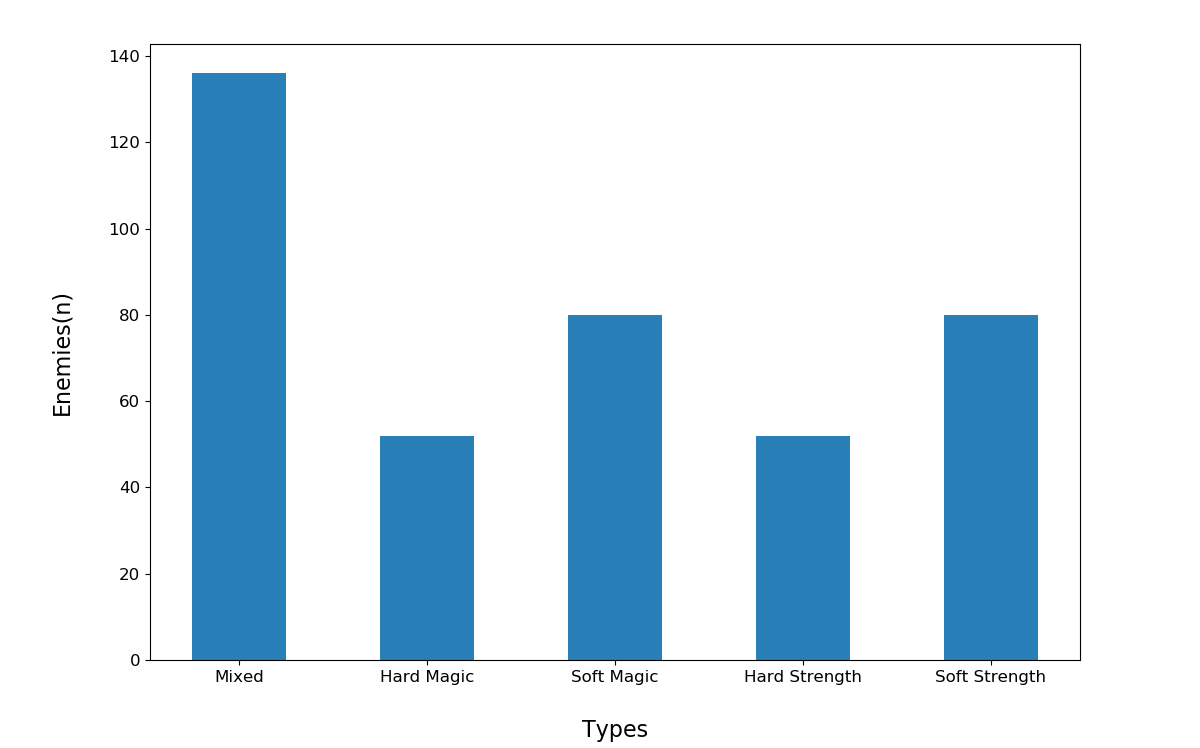
\includegraphics[scale=0.5]{img/EnemyTypeDistrib.png}
	\caption{Distribusi tipe musuh.}
	\label{fig:enemy_type_distrib}
\end{figure}

Kemudian pada Gambar \ref{fig:enemy_type_distrib} adalah hasil dari proses pembuatan dan pengelompokan musuh berdasarkan tipe yang sudah sesuai dengan variabel masukan pada Tabel \ref{tb:enemy_input_variable}. Dengan musuh bertipe \textit{Mixed} berjumlah yang paling banyak, diikuti \textit{soft magic} dan \textit{soft strength} dengan harapan bahwa ini adalah musuh yang memiliki karakter \textit{magic} dan \textit{strength} namun masih mudah dikalahkan, dilanjutkan dengan yang paling sedikit adalah \textit{hard magic} dan \textit{hard strength} dengan harapan menjadi musuh berkarakter strength dan magic yang sulit dikalahkan.
\vspace{1ex}

\subsection{Distribusi Elemen dan Kelemahan Musuh}
\label{sec:sub_sec3_enemy_weak}
\vspace{1ex}

Pada persamaan \ref{eq:enemy_element} adalah penjelasan elemen yang digunakan oleh musuh seperti dideskripsikan pada Tabel \ref{tb:enemy_input_variable} pada variabel \textit{List Element}, di mana pada elemen teresebut terdapat kelemahan atau \textit{weaknesses} dan kekebalan atau \textit{repel} seperti yang dideskripsikan pada variabel \textit{List Damage} pada Tabel \ref{tb:enemy_input_variable}.  Seperti yang dijelaskan pada Sub-bab \ref{sec:sub_sec3_design_skenario} poin ke dua tentang Elemen dan Efektifitas Serangan. Pada bagian ini elemen tersebut akan dibagi ke setiap musuh dengan kondisi yang berbeda, maksudnya nanti akan ada musuh yang memiliki kelemahan dan kekebalan yang berbeda antara musuh satu dengan musuh yang lain. Misalkan \textit{Enemy 1} memiliki kelemahan api atau \textit{fire} yang mana HP akan berkurang dua kali jika diserang dengan menggunakan elemen api dan memiliki kekebalan air atau \textit{water} yang mana karakter tersebut kebal saat diserang dengan \textit{skill} dari elemen air. Kemudian pada \textit{Enemy 2} berbeda dengan \textit{Enemy 1}, misalnya pada \textit{Enemy 1} memiliki kelemahan api sedangkan pada \textit{Enemy 2} memiliki kelemahan air misal dan kebal terhadap angin atau \textit{wind}.

\begin{equation}\label{eq:enemy_element}
\resizebox{0.2\textwidth}{!}{%
	$ElN = \left\{\begin{matrix}
	\hspace{-0.34em} Phys \\ 
	\hspace{0.3em} Water \\
	\hspace{0.0em} Wind \\
	\hspace{0.2em} Earth \\
	\hspace{-0.3em} Fire \\
	\hspace{-1.6em} ... \\
	\hspace{-1.6em} n
	\end{matrix}\right.$%
}
\end{equation}

Pada dasarnya satu karakter musuh tidak akan menggunakan seluruh elemen yang ada pada persamaan \ref{eq:enemy_element} yang merupakan penggambaran dari varaibel \textit{List Element} pada Tabel \ref{tb:enemy_input_variable}, mungkin hanya sekitar satu sampai dengan tiga. Maka dari itu kondisi tersebut dapat dinyatakan dengan kondisi $DmgNa \in ElN$, yang mana seluruh elemen bisa menjadi kelemahan atau kekebalan dari musuh. Sama seperti pada persamaan \ref{eq:enemy_element} yang mana $ElN$ adalah nama elemen, sedangkan $DmgNa$ adalah \textit{damage name} atau nama dari efek serangan yang dilakukan. Di mana pada persamaan \ref{eq:damage_name_number} $DmgNa$ akan dipilih secara acak dengan persamaan \ref{eq:damage_number_prob}, yang akan menjadi kelemahan atau kekebalan terhadap serangan dari pemain seperti pada persamaan \ref{eq:damage_name_number}. Pada persamaan \ref{eq:damage_name_number} sendiri adalah penggambaran dari variabel \textit{List Damage} pada Tabel \ref{tb:enemy_input_variable}. 

\begin{equation}\label{eq:damage_name_number}
\resizebox{0.5\textwidth}{!}{%
	$DmgNu = \left\{\begin{matrix} 
	\hspace{0.0em} 0,  & \hspace{-7.0em} Normal \\
	\hspace{0.0em} 1,  & \hspace{-8.0em} Repel \\
	\hspace{0.0em} 2,  & \hspace{-7.7em} Weak \\
	\hspace{0.5em} ... & \\
	\hspace{0.5em} n,  & Defined\ Status\ Name
	\end{matrix}\right.$%
}
\end{equation}

Sedangkan pada persamaan \ref{eq:damage_name_number} variabel $DmgNu$ adalah respon terhadap serangan yang yang dikonversi menjadi angka, yang pada mulanya berupa nama respon atau status setelah diserang. Kemudian hasil pemilihan tersebut disimpan pada variabel $DmgNu$ yang dapat dinyatakan dengan persamaan \ref{eq:damage_number_prob}.

\begin{equation}\label{eq:damage_number_prob}
P(DmgNu) = \frac{DmgNu}{\sum_{i = 0}^{N}\ DmgNa_{(i - 1)}}
\end{equation}

Pada persamaan \ref{eq:damage_name_number} variabel $DmgNa$ yang dipilih secara acak sebagai elemen yang memiliki respon khusus terhadap serangan yang kemudian disimpan pada variabel $DmgNu$, selanjutnya angka yang dipilih akan disimpan pada variabel $DmgNu$ yang selanjutnya dinyatakan dengan persamaan \ref{eq:damage_number_prob}. Jadi dari $DmgNa$ akan dipilih satu sampai dengan tiga elemen secara acak yang kemudian menjadi kelemahan atau kekebalan dari karakter musuh tersebut.

\begin{equation}\label{eq:multi_damage_num_prob}
P(DmgNu)_{M} = \sum_{i = 0}^{M}\ \frac{DmgNu_{i}}{\sum_{j = 0}^{N}\ DmgNa_{j - 1}}
\end{equation}

Sedangkan pada persamaan \ref{eq:multi_damage_num_prob} adalah penjelasan tentang proses munculnya setiap $DmgNu$ pada satu karakter musuh, sehingga variabel tersebut berubah menjadi $DmgNu_{i}$. Seperti penjelasan sebelumnya bahwa pada sebuah karakter musuh dapat memiliki lebih dari satu kelemahan atau kekebalan $DmgNu$ terhadap $DmgNa$ yang diset secara acak seperti yang sudah dijelaskan pada bagian sebelumnya.

\begin{equation}\label{eq:all_enemies_damage}
DmgEN_{M} = \sum_{i = 0}^{M}\sum_{j = 0}^{N} DmgNu_{ij}
\end{equation}

Selanjutnya adalah proses penerapan persamaan \ref{eq:multi_damage_num_prob} ke seluruh karakter musuh $DmgEN_{M}$ seperti pada persamaan \ref{eq:all_enemies_damage}. Sesuai dengan persamaan \ref{eq:all_enemies_damage}, yang mana $M$ adalah jumlah musuh sedangkan $N$ adalah jumlah $DmgNu$ pada satu musuh yang berjumlah satu sampai dengan tiga seperti yang sudah dijelaskan pada paragraf sebelumnya pada Sub-bab ini. Hasil dari proses dari keseluruhhan proses yang dijelaskan pada Sub-bab ini menghasilkan persebaran kelemahan dan kekebalan musuh yang ditunjukkan pada Tabel \ref{tb:enemy_weak_distrib}.
\vspace{1ex}

\begin{table}[!h]
	\centering
	\caption{Hasil level yang dibuat untuk musuh.}
	\label{tb:enemy_weak_distrib}
	\begin{tabular}{|l|l|l|l|l|l|l|}
		\hline
		\textbf{No.} & \textbf{Name} & \textbf{Phys} & \textbf{Water} & \textbf{Wind} & \textbf{Earth} & \textbf{Fire} \\ \hline
		1 & Enemy 1 & 1 & 0 & 1 & 1 & 0 \\ \hline
		2 & Enemy 2 & 0 & 0 & 0 & 0 & 0 \\ \hline
		3 & Enemy 3 & 0 & 2 & 1 & 1 & 1 \\ \hline
		4 & Enemy 4 & 1 & 1 & 0 & 0 & 0 \\ \hline
		5 & Enemy 5 & 0 & 2 & 1 & 0 & 1 \\ \hline
		6 & Enemy 6 & 1 & 1 & 1 & 1 & 0 \\ \hline
		7 & Enemy 7 & 1 & 2 & 0 & 0 & 0 \\ \hline
		8 & Enemy 8 & 0 & 0 & 0 & 0 & 1 \\ \hline
		9 & Enemy 9 & 1 & 2 & 1 & 0 & 0 \\ \hline
		10 & Enemy 10 & 0 & 2 & 0 & 0 & 0 \\ \hline
		11 & Enemy 11 & 1 & 4 & 0 & 1 & 0 \\ \hline
		12 & Enemy 12 & 0 & 0 & 0 & 0 & 1 \\ \hline
		13 & Enemy 13 & 0 & 0 & 0 & 1 & 0 \\ \hline
		14 & Enemy 14 & 0 & 4 & 1 & 0 & 0 \\ \hline
		15 & Enemy 15 & 0 & 4 & 2 & 1 & 0 \\ \hline
		... & ... & ... & ... & ... & ... & ... \\ \hline
		\textbf{400} & \textbf{Enemy 400} & \textbf{0} & \textbf{0} & \textbf{2} & \textbf{1} & \textbf{0} \\ \hline
	\end{tabular}
\end{table}
\vspace{1ex}

Jika melihat Tabel \ref{tb:enemy_weak_distrib} Hasil dari proses yang sebelumnya dijelaskan pada Sub-bab ini menghasilkan persebaran kelemahan dan kekebalan musuh yang ditunjukkan pada Gambar \ref{fig:enemy_weak_distrib} dibawah ini.

\begin{figure} [!h] \centering
	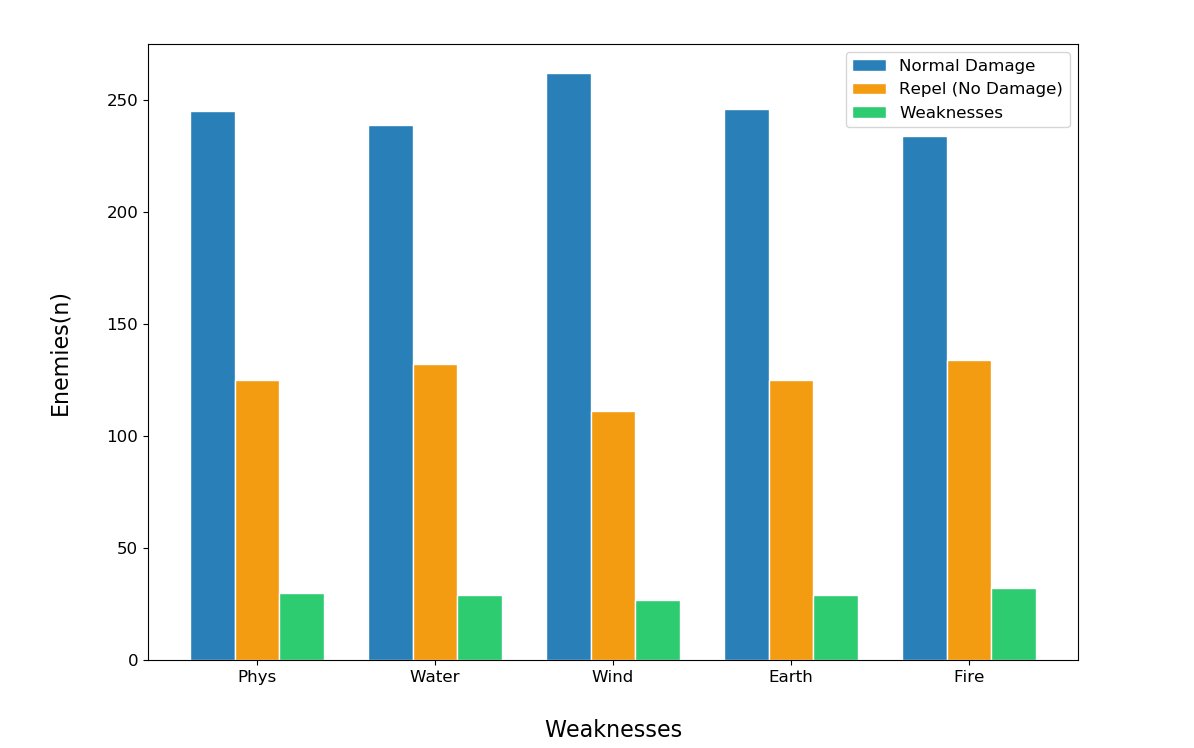
\includegraphics[scale=0.50]{img/EnemyWeakDistrib.png}
	\caption{Distribusi kelemahan musuh.}
	\label{fig:enemy_weak_distrib}
\end{figure}

Pada Gambar \ref{fig:enemy_weak_distrib} dapat dilihat distribusi musuh dengan kelemahan dan kekebalannya. Terlihat pada kondisi tersebut jumlah musuh dengan kondisi \textit{Normal} memiliki nilai paling tunggi pada setiap kelemahan, hal tersebut dapat diartikan bahwa sebagian besar elemen dari musuh dapat memperoleh \textit{damage} secara normal jika diserang. Kemudian jumlah musuh pada kondisi \textit{Repel} berjumlah terbanyak kedua, hal tersebut dapat diartikan musuh memmiliki jumlah kekebalan terhadap serangan sejumlah angka pada setiap elemen pada Gambar \ref{fig:enemy_weak_distrib}. Begitu juga dengan kondisi \textit{Weaknesses} dengan jumlah paling sedikit, hal tersebut bertujuan agar menjadikan pertarungan antara pemain dan musuh menjadi tidak mudah dimenangkan oleh pemain. Tidak hanya dengan efek \textit{Weaknesses}, efek \textit{Repel} juga sangat berpengaruh dalam menjadikan permainan seperti layaknya sebuah \textit{puzzle} atau teka-teki.
\vspace{1ex}

Sedangkan pada persamaan \ref{eq:multi_damage_num_prob} adalah penjelasan tentang proses munculnya setiap $DmgNu$ pada satu karakter musuh, sehingga variabel tersebut berubah menjadi $DmgNu_{i}$. Seperti penjelasan sebelumnya bahwa pada sebuah karakter musuh dapat memiliki lebih dari satu kelemahan atau kekebalan $DmgNu$ terhadap $DmgNa$ yang diset secara acak seperti yang sudah dijelaskan pada bagian sebelumnya. 
\vspace{1ex}

\subsection{Distribusi HP, MP dan Stats Musuh}
\label{sec:sub_sec3_enemy_hp_mp_stats}
\vspace{1ex}

Bila melihat pada Tabel \ref{tb:enemy_input_variable} terdapat beberapa variabel seperti \textit{List Stats Name}, \textit{Max Stats Value}, dan \textit{Min Stats Value}. Variabel tersebut akan digunakan untuk membuat \textit{stats} dari musuh dengan basis algorima Naive Bayes. Di awali dengan persamaan \ref{eq:enemy_types_stats_ex} yang menjadi pembagi setiap operasi pembagian \textit{stats} berdasarkan tipenya $ET_{i}$.

\begin{equation}\label{eq:enemy_types_stats_ex}
\resizebox{0.4\textwidth}{!}{%	
	$ET_{N} = \sum_{i= 0}^{N} ET_{i} \left\{\begin{matrix}
	ET_{i} = 0, & MX\\ 
	ET_{i} = 1, & HM\\ 
	ET_{i} = 2, & SM\\ 
	ET_{i} = 3, & HS\\ 
	ET_{i} = 4, & SS
	\end{matrix}\right.$%
}
\end{equation}

Pada persamaan \ref{eq:enemy_types_stats_ex} adalah persamaan yang disesuaikan untuk menyelesaikan masukan variabel pada Tabel \ref{tb:enemy_input_variable}, sedangkan pada persaamaan \ref{eq:enemy_types_stats_adv} adalah pengembangan jika jumlah tipe musuh dinaikkan lebih dari yang dicontohkan pada Tabel \ref{tb:enemy_input_variable} pada variabel \textit{Enemy Type}.
\vspace{1ex}

\begin{equation}\label{eq:enemy_types_stats_adv}
\resizebox{0.4\textwidth}{!}{%
	$ET_{N} = \sum_{i= 0}^{N} ET_{i} \left\{\begin{matrix}
	ET_{i} = 0, & MX\\ 
	ET_{i} = 1, & HM\\ 
	ET_{i} = 2, & SM\\ 
	ET_{i} = 3, & HS\\ 
	ET_{i} = 4, & SS\\
	... & ... \\
	\hspace{0.2em} ET_{n} = n, & ST_{n}
	\end{matrix}\right.$%
}
\end{equation}

Pada kedua persamaan tersebut terdaapat beberapa variabel diantaranya adalah $ET_{i}$ yang merupakan enemy tipe ke $i$, kemudian secara berurutan masing-masing $MX$, $HM$, $SM$, $HS$, dan $SS$ adalah musuh dengan tipe \textit{mixed}, \textit{hard magic}, \textit{soft magic}, \textit{hard strength}, dan \textit{soft strength}. Kemudian pada persamaan \ref{eq:enemy_types_stats_adv} secara spesifik terdapat variabel $ET_{n}$ yang merupakan variabel tipe musuh ke $n$ atau batas jumlah musuh. Variabel $n$ adalah urutan dari index tipe musuh yang dideskripsikan, berikut juga variabel $ST_{n}$, dengan variabel $ST$ adalah \textit{stats} dan $n$ adalah batas jumlah musuh. Selanjutnya adalah dilakukannya pembagian tipe musuh jika musuh tersebut memiliki tipe $MX$ atau \textit{mixed} seperti pada persamaan \ref{eq:enemy_types_stats_mixed_ex}.
\vspace{1ex}

\begin{equation}\label{eq:enemy_types_stats_mixed_ex}
MX_{N} = \sum_{i= 0}^{N} MX_{i} \left\{\begin{matrix}
MX_{i} = 1, & MP\ Focused\\
MX_{i} = 2, & HP\ Focused
\end{matrix}\right.
\end{equation}

Pada persamaan \ref{eq:enemy_types_stats_mixed_ex} terdapat variabel $MX_{i}$ yang merupakan variabel satuan dari musuh yang bertipe \textit{mixed}. Kemudian pada variabel $MX_{N}$ adalah variabel yang bersifat jamak atau memuat banyak variabel musuh yang bertipe \textit{mixed}. Pada persamaan \ref{eq:enemy_types_stats_mixed_ex} sendiri dijelaskan bahwa pada tipe \textit{mixed} dipecah menjadi dua tipe lagi, yang satu berfokus pada $HP$ dan satu lagi pada $MP$. Jadi isi dari variabel $MX_{N}$ nantinya akan terdiri dari musuh bertipe \textit{mixed} dengan sub-tipe MP atau berfokus pada MP dan sub-tipe HP atau berfokus pada HP.

\begin{equation}\label{eq:enemy_types_stats_mixed_adv}
Mx_{N} = \sum_{i= 0}^{N} Mx_{i} \left\{\begin{matrix}
\hspace{0.6em} Mx_{i} = 1, & MP\ Focused\\
\hspace{0.6em} Mx_{i} = 2, & HP\ Focused\\
\hspace{0.6em} ... & \hspace{-2.0em} ... \\
\hspace{0.8em} Mx_{N} = n, & \hspace{-2.0em} Lainnya\\
\end{matrix}\right.
\end{equation}

Selanjutnya adalah perhitungan probabilitas diperolehnya tipe musuh dari keseluruhan tipe musuh yang berada pada variabel masukan. Misal pada kasus yang ditunjukan pada persamaan \ref{eq:enemy_types_prob_ex}, jumlah tipe musuh tentunya mengacu pada Tabel \ref{tb:enemy_input_variable}. Dalam menyelesaikan kasus tersebut digunakanlah Naive bayes yang berbasis pada \textit{conditional probability} seperti yangg dijelaskan pada Sub-bab \ref{sec:sub_sec2_class_bayes}, yang mana pada persamaan \ref{eq:enemy_types_prob_ex} proses kemunculan tipe musuh tertentu misal $ET_{0}$, $ET_{1}$, $ET_{2}$, $ET_{3}$, $ET_{4}$ yang mana seluruh tipe musuh dimuat pada variabel $ET_{N}$.

\begin{equation}\label{eq:enemy_types_prob_ex}
\resizebox{0.35\textwidth}{!}{%
	$\begin{matrix}
	ET_{0} = P(ET_{N}| ET_{0}) \times P(ET_{0})\\
	ET_{1} = P(ET_{N}| ET_{1}) \times P(ET_{1})\\
	ET_{2} = P(ET_{N}| ET_{2}) \times P(ET_{2})\\
	ET_{3} = P(ET_{N}| ET_{3}) \times P(ET_{3})\\
	ET_{4} = P(ET_{N}| ET_{4}) \times P(ET_{4})
	\end{matrix}$%
}
\end{equation}

Sedangkan jika jumlah tipe musuh tidak beracuan pada Tabel \ref{tb:enemy_input_variable} atau tipe musuh berjumlah lebih dari empat maka persamaan \ref{eq:enemy_types_prob_ex} akan berubah menjadi persamaan \ref{eq:enemy_types_prob_adv}. Semula berawal dari variabel $ET_{0}$ sampai $ET_{4}$ pada persamaan \ref{eq:enemy_types_prob_ex} yang kemudian berubah dari variabel $ET_{0}$ sampai $ET_{n}$ dengan $n$ adalah batas akhir jumlah tipe musuh.

\begin{equation}\label{eq:enemy_types_prob_adv}
\resizebox{0.35\textwidth}{!}{%
	$\begin{matrix}
	ET_{0} = P(ET_{N}| ET_{0}) \times P(ET_{0})\\
	ET_{1} = P(ET_{N}| ET_{1}) \times P(ET_{1})\\
	ET_{2} = P(ET_{N}| ET_{2}) \times P(ET_{2})\\
	...\\
	ET_{n} = P(ET_{N}| ET_{n}) \times P(ET_{n})
	\end{matrix}$%
}
\end{equation}

Saat sudah diperolehnya tipe musuh pada seperti yang dijelaskan pada persamaan \ref{eq:enemy_types_prob_adv} maka selanjutnya yang harus dibuat adalah stats dari musuh itu sendiri, seperti halnya HP, MP, Strength, Magic dan lain sebagainya seperti yang tercantum pada Tabel \ref{tb:enemy_input_variable} pada variabel $List Stats Name$ yang ditambah dengan variabel HP dan MP.

\begin{equation}\label{eq:enemy_types_prob_bhp}
bHP = minHP
\end{equation}

Pada persamaan \ref{eq:enemy_types_prob_bhp} adalah penentuan batas bawah untuk HP atau $bHP$, nilai $minHP$ juga dicontohkan dalam daftar variabel masukan dengan nama \textit{Min} HP pada Tabel \ref{tb:enemy_input_variable}.

\begin{equation}\label{eq:enemy_types_prob_thp}
tHP = \sum_{i=0}^{N}\ bHP + \left |\ \frac{Elv_{i}}{100} \times maxHP\ \right |
\end{equation}

Selanjutnya dilanjutkan dengan pencarian batas atas untuk HP atau $tHP$. Pada persamaan \ref{eq:enemy_types_prob_thp} terdapat beberapa variabel yang berpengaruh terhadap nilai dari $tHP$ diantaranya adalah $bHP$ yang merupakan batas bawah dari $HP$, $Elv_{i}$ yang merupakan level dari setiap karakter musuh dengan tipenya masing-masing, dan $maxHP$ sendiri yang merupakan batas atas dicontohkan pada Tabel \ref{tb:enemy_input_variable} dengan nama variabel $max$ HP. Pencarian batas atas dilakukan dengan dilakukannya penjumlahan antara $bHP$ dengan presentase dari $maxHP$ yang disesuaikan dengan $Elv_{i}$. Jadi dari perhitungan tersebut HP dari karakter musuh akan menyesuikan dengan level pada karakter musuh tersebut. 

\begin{equation}\label{eq:enemy_types_prob_hp}
P(HP_{i}) = \sum_{i=0}^{N}\ \frac{HP_{i}}{bHP_{i} - tHP_{i}}
\end{equation}

Kemdian dilanjutkan dengan perhitungan probabilitas $P(HP_{i})$ atau munculnya HP pada setiap karakter musuh pada persamaan \ref{eq:enemy_types_prob_hp}. HP dari setiap karakter musuh itu sendiri dinyatakan dengen $HP_{i}$. Kemudian range nilai dari $HP_{i}$ yang akan muncul terhitung mulai dari $bHP_{i}$ sampai dengan $tHP_{i}$ dari setiap karakter musuh. Variabel $i$ pada persamaan tersebut merepresentasikan setiap musuh dengan variabel $N$ yang menyatakan batas atau jumlah dari musuh yang ingin dibuat.

\begin{equation}\label{eq:enemy_types_prob_bmp}
bMP = minMP
\end{equation}

Mengulang persamaan \ref{eq:enemy_types_prob_bhp} pada persamaan \ref{eq:enemy_types_prob_bmp}, hanya mengganti variabelnya saja. Jika pada persamaan \ref{eq:enemy_types_prob_bhp} kasus yang ingin diselesaikan adalah pencariaan \textit{stats} HP, maka pada persamaan \ref{eq:enemy_types_prob_bmp} kasus yang ingin diselesaikan adalah pencarian \textit{stats} MP. Pada persamaan \ref{eq:enemy_types_prob_bhp} dengan variabel $bHP$ diganti dengan $bMP$ dan variabel $minHP$ diganti dengan $minMP$ yang mana pada Tabel \ref{tb:enemy_input_variable} dicontohkan dengan variabel $Min$ MP.
\vspace{1ex}

\begin{equation}\label{eq:enemy_types_prob_tmp}
tMP = \sum_{i=0}^{N}\ bMP + \left |\ \frac{Elv_{i}}{100} \times maxMP\ \right |
\end{equation}

Masih sama seperti penjelasan sebelumnya dimana pada persaamaan \ref{eq:enemy_types_prob_bmp} pada persamaan \ref{eq:enemy_types_prob_tmp} juga sama dengan persamaan \ref{eq:enemy_types_prob_thp}. Di lakukannya penggantian variabel HP menjadi MP, sudah dijelaskan juga pada bagian sebelumnya tentang variabel $Elv_{i}$, dan pada variabel $maxMP$ yang merupakan variabel yang dicontohkan pada Tabel \ref{tb:enemy_input_variable} dengan nama \textit{Max} MP.

\begin{equation}\label{eq:enemy_types_prob_mp}
P(MP_{i}) = \sum_{i=0}^{N}\ \frac{MP_{i}}{bMP_{i} - tMP_{i}}
\end{equation}

Pada persamaan \ref{eq:enemy_types_prob_mp} adalah probabilitas $P(MP_{i})$ atau munculnya MP pada setiap karakter musuh pada persamaan \ref{eq:enemy_types_prob_mp}. MP dari setiap karakter musuh itu sendiri dinyatakan dengen $MP_{i}$. Kemudian range nilai dari $MP_{i}$ yang akan muncul terhitung mulai dari $bMP_{i}$ sampai dengan $tMP_{i}$. Kasus ini sama seperti pada persamaan \ref{eq:enemy_types_prob_hp} hanya saja sama seperti pada pembahasan sebelumnya yang mana pada persamaan tersebut bertujuan untuk mencari $HP$, sedangkan pada kasus ini bertujuan untuk mencaru $MP$.
\vspace{1ex}

Pada bagian ini akan membahas secara khusus untuk kondisi \textit{mixed} melanjutkan seperti yang ada pada persamaan \ref{eq:enemy_types_stats_mixed_ex}. Dalam kondisi \textit{mixed} sendiri terdapat dua kondisi yaitu HP \textit{focused} atau yang berfokus kepada HP, kemudian MP \textit{focused} atau yang befokus pada MP. Bila masing-masing tipe tersebut dinyatakan dengan persamaan secara berurutan untuk HP \textit{focused} dan MP \textit{focused} dengan persamaan \ref{eq:enemy_types_prob_mx1} dan persamaan \ref{eq:enemy_types_prob_mx2}. 

\begin{equation}\label{eq:enemy_types_prob_mx1}
Mx_{1} = P(Mx_{{N}}|Mx_{1}) \times P(Mx_{1})
\end{equation}

Maka $Mx_{N}$ adalah seluruh musuh yang bertipe $mixed$, kemudian dipilihlah musuh dengan tipe mixed yang berfokus pada HP atau $Mx_{1}$. Beracuan pada konsep \textit{conditional probability} yang sudah dijelaskan pada Sub-bab \ref{sec:sub_sec2_bayes}.

\begin{equation}\label{eq:enemy_types_prob_mx2}
Mx_{2} = P(Mx_{{N}}|Mx_{2}) \times P(Mx_{2})
\end{equation}

Jika $Mx_{1}$ adalah HP \textit{focused} maka  $Mx_{2}$ adalah MP \textit{focused} maka sama seperti persamaan \ref{eq:enemy_types_prob_mx1} dengan $Mx_{N}$ adalah seluruh musuh yang bertipe $mixed$, kemudian dipilihlah musuh dengan tipe \textit{mixed} yang berfokus pada MP atau $Mx_{2}$. Pembahasan secara khusus lainnya adalah penambahan \textit{stats} HP untuk musuh dengan tipe \textit{mixed} yang berfokus pada HP seperti yang dinyatakan pada persamaan \ref{eq:enemy_types_prob_thp_mix}. Sedangkan pada musuh dengan tipe \textit{mixed} yang berfokus pada MP tidak perlu diberi perlakuan khusus seperti tipe \textit{mixed} yang berfokus pada HP, hal tersebut dikarenakan dengan melihat nilai MP pada setiap karakter musuh dengan tipe tersebut sudah tergolong tinggi. Kondisi ini beracuan terhadap konsep keseimbangan dalam mendesain seperti yang dijelaskan pada Sub-bab \ref{sec:sub_sec2_keseimbangan} dan Sub-bab \ref{sec:sub_sec3_story} tentang penyesuaian keseimbangan dalam pertarungan antara pemain dengan musuh berikut juga dengan cerita dari permainan tersebut.

\begin{equation}\label{eq:enemy_types_prob_thp_mix}
tHP = \sum_{i=0}^{N}\ bHP + bHP + \left | \frac{Elv_{i}}{100} \times maxHP \right |
\end{equation}

Sedikit berbeda dengan persamaan \ref{eq:enemy_types_prob_hp} pada persaamaan \ref{eq:enemy_types_prob_thp_mix} dilakukan penambahan dua kali pada variabel $bHP$ atau batas bawah HP. Hal tersebut dilakukan agar angka \textit{stats} HP pada musuh dengan tipe \textit{mixed} yang berfokus terhadap HP memiliki nilai HP yang lebih tinggi jika dibandingkan dengan tipe \textit{mixed} yang berfokus MP.

\begin{equation}\label{eq:enemy_types_prob_hp_mix}
P(HP_{i}) = \sum_{i=0}^{N}\ \frac{HP_{i}}{bHP_{i} - tHP_{i}}
\end{equation}

Kemudian perhitungan probabilitas $P(HP_{i})$ atau munculnya HP pada setiap karakter musuh pada persamaan \ref{eq:enemy_types_prob_hp_mix}. HP dari setiap karakter musuh itu sendiri dinyatakan dengen $HP_{i}$. Kemudian range nilai dari $HP_{i}$ yang akan muncul terhitung mulai dari $bHP_{i}$ sampai dengan $tHP_{i}$. Persamaan tersebut masih sama dengan probabilitas kemunculan HP dari \textit{range} antara $bHP$ dengan $tHP$ pada persamaan \ref{eq:enemy_types_prob_hp}.
\vspace{1ex}

Selain pembuatan \textit{stats} HP dan MP, \textit{stats} lain seperti halnya \textit{Strength}, \textit{Magic}, \textit{Endurance}, \textit{Speed} dan \textit{Luck} juga harus dicari. Daftar dari \textit{stats} tersebut dicontohkan pada Tabel \ref{tb:enemy_input_variable} dengan nama variabel \textit{List Stats Name}. Dalam kasus pembuatan \textit{stats} musuh terdapat beberapa variabel lain digunakan selain \textit{List Stats Name} diantaranya adalah \textit{Max Stats Value} dan \textit{Min Stats Value}, seperti yang ditunjukan pada Tabel \ref{tb:enemy_input_variable}. Dalam pembuatan \textit{stats} musuh tersebut digunakanlah persamaan yang mirip dengan persamaan \ref{eq:enemy_types_prob_bhp}, \ref{eq:enemy_types_prob_thp}, dan persamaan \ref{eq:enemy_types_prob_hp}, hanya saja dilakukan sedikit perubahan pada persamaan tersebut seperti yang dinyatakan pada persamaan \ref{eq:enemy_types_prob_bst1}, \ref{eq:enemy_types_prob_bst2}, \ref{eq:enemy_types_prob_tst1}, \ref{eq:enemy_types_prob_tst2}, dan persamaan \ref{eq:enemy_types_prob_st}.

\begin{equation}\label{eq:enemy_types_prob_bst1}
bSt = minSt
\end{equation}

Jika hanya berlaku satu \textit{stats} saja maka dapat digunakan persamaan \ref{eq:enemy_types_prob_bst1} yang pada dasarnya sama seperti persamaan-persamaan sebelumnya dalam mencari batas bawah dari HP pada $bHP$ dan MP pada $bMP$. Sedangkan pada persamaan \ref{eq:enemy_types_prob_bst1} batas bawahnya adalah $bSt$ yang diisi dengan nilai minimum dari \textit{stats} atau $minSt$.

\begin{equation}\label{eq:enemy_types_prob_bst2}
bSt_{i} = \sum_{i=0}^{N}\ minSt_{i}
\end{equation}

Di karenakan \textit{stats} dari musuh berjumlah lebih dari satu maka persamaan \ref{eq:enemy_types_prob_bst1} harus disesuaikan dengan jumlah \textit{stats} tersebut. Jumlah stats dari musuh sendiri berjumlah lima buah seperti yang tertulis pada variabel \textit{List Stats Name}, maka persamaan \ref{eq:enemy_types_prob_bst1} disesuaikan menjadi seperti persamaan \ref{eq:enemy_types_prob_bst2}. Dengan variabel $N$ adalah batas maksimal dari jumlah \textit{stats}, dengan nilai minimum \textit{stats} atau $minSt$ yang jumlahnya mengikuti jumlah maksimal \textit{stats} menjadi $minSt_{i}$ dan disimpan dalam setiap variabel $bSt$ ke $i$. Kemudian selanjutnya adalah pencarian batas atas untuk masing-masing \textit{stats}, sama halnya dengan pencarian batas bawah dari setiap \textit{stats} dalam cara pencarian batas atas pada dasarnya juga sama dengan pencarian batas dari HP pada $tHP$ dan MP pada $tMP$.

\begin{equation}\label{eq:enemy_types_prob_tst1}
tSt_{i} = \sum_{i=0}^{N}\ bSt + \left |\ \frac{Elv_{i}}{100} \times maxSt_{i}\ \right |
\end{equation}

Pada persamaan \ref{eq:enemy_types_prob_tst1} batas atasnya adalah $tSt$ yang diisi dengan nilai maximum dari \textit{stats} atau $maxSt$. Namun pada kasus ini jumlah \textit{stats} musuh berjumlah lebih dari satu seperti yang sudah dibahas pada bagian sebelumnya. Sama seperti pada pembahasan sebelumnya bahwa variabel $N$ adalah jumlah \textit{stats} musuh, maka dari itu nilai maksimum $maxSt$ dan variabel penyimpan hasil batas maksimum $tSt$ dieksekusi sesuai satu-satu sesuai jumlah \textit{stats} maka masing-masing variabel tersebut secara berurutan menjadi $maxSt_{i}$ dan $tSt_{i}$.

\begin{equation}\label{eq:enemy_types_prob_tst2}
tSt_{i} = \sum_{i=0}^{N}\ bSt_{i} + \left |\ \frac{Elv_{i}}{100} \times maxSt_{i}\ \right |
\end{equation}

Dalam pencarian nilai batas atas $tSt_{i}$ tentunya harus melibatkan batas bawah. Jika melihat pada persamaan \ref{eq:enemy_types_prob_tst1} maka terdapat variabel $bSt$, tapi pada variabel tersebut masih bersifat statis atau tidak menyesuaikan dengan jumlah \textit{stats} musuh. Digabunglah persamaan \ref{eq:enemy_types_prob_bst2} dengan persamaan \ref{eq:enemy_types_prob_tst1} sehingga diperolehnya persamaan \ref{eq:enemy_types_prob_tst2} dengan variabel $bSt$ yang mengikuti jumlah \textit{stats} musuh menjadi $bSt_{i}$ dengan variabel $N$ sebagai batasan maksimal jumlah \textit{stats}. Dengan varaiabel $i$ yang merepresentasikan urutan \textit{stats} musuh yang sedang diproeses. Penjelasan untuk persamaan ini sebenarnya sama seperti persamaan \ref{eq:enemy_types_prob_thp} hanya saja jumlah \textit{stats} yang dibuat lebih banyak.

\begin{equation}\label{eq:enemy_types_prob_st}
P(St_{i}) = \sum_{i=0}^{N}\ \frac{St_{i}}{bSt_{i} - tSt_{i}}
\end{equation}

Kemudian pada persamaan \ref{eq:enemy_types_prob_st} adalah probabilitas $P(St_{i})$ saat munculnya \textit{stats} $St_{i}$ dari batas bawah \textit{stats} $bSt_{i}$ sampai batas atas \textit{stats} $tSt_{i}$. \textit{Stats} dari setiap karakter musuh berhasil dibuat melalui banyak langkah pada Sub-bab ini, diantaranya adalah \textit{Strength}, \textit{Magic}, \textit{Endurance}, \textit{Speed}, dan \textit{Luck}. Dari keseluruhan \textit{stats} tersebut bila digabungkan maka hasilnya dapat dilihat pada Gambar \ref{fig:enemy_all_stats_distrib}.

\begin{figure} [!h] \centering
	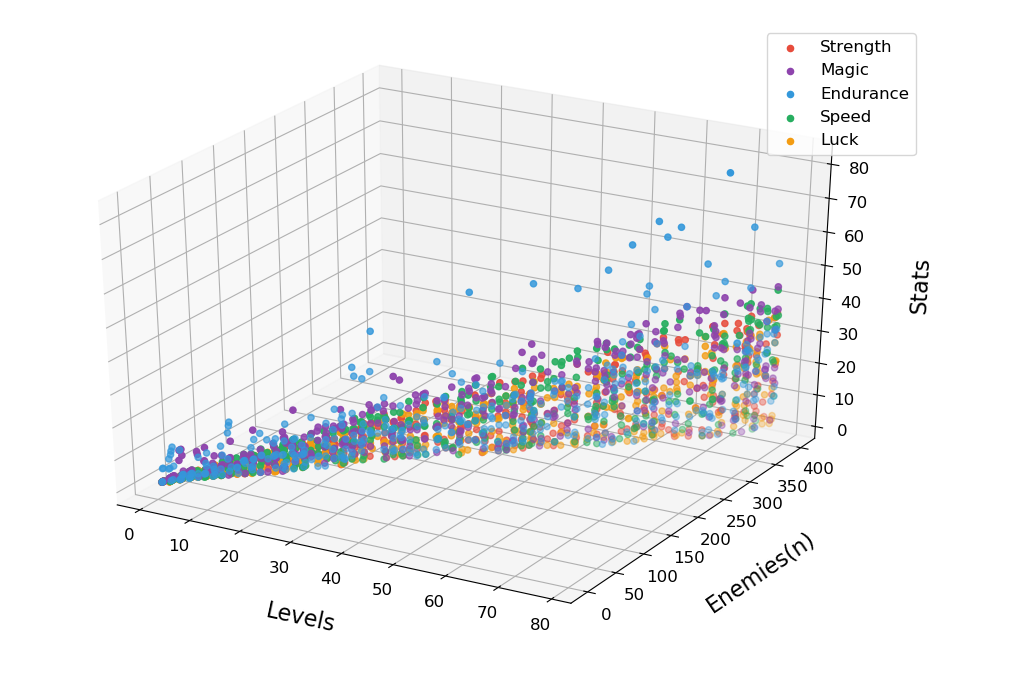
\includegraphics[scale=0.59]{img/EnemyStatsDistrib.png}
	\caption{Distribusi \textit{stats} musuh secara keseluruhan.}
	\label{fig:enemy_all_stats_distrib}
\end{figure}

Selanjutnya adalah penggambaran persebaran \textit{stats} HP dan MP yang masing-masing dijabarkan pada persamaan \ref{fig:enemy_hp_distrib} dan persamaan \ref{fig:enemy_mp_distrib}. Sama seperti pada persamaan \ref{fig:enemy_all_stats_distrib}, yang mana pada persamaan \ref{fig:enemy_hp_distrib} dan persamaan \ref{fig:enemy_mp_distrib} divisualisasikan secara ke dalam bentuk tiga dimensi. Hal tersebut dilakukan agar terciptanya perbandingan antara level, jumlah musuh, dan tingkat tingginya nilai \textit{stats} yang bersangkutan.

\begin{figure} [!h]
\begin{minipage}[t]{1.0\linewidth}
	\centering
	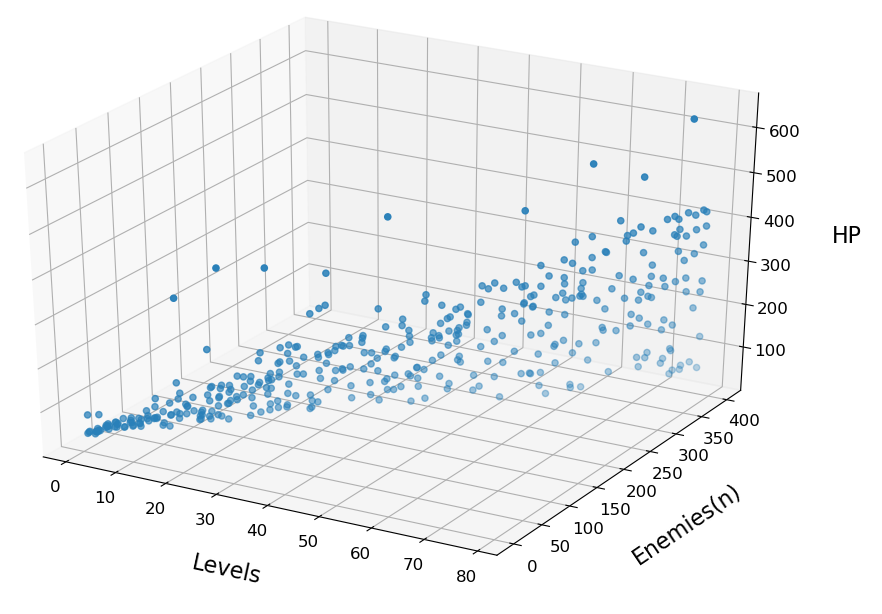
\includegraphics[scale=0.58]{img/EnemyHpDistrib.png}
	\caption{Distribusi \textit{stats} HP musuh.}
	\label{fig:enemy_hp_distrib}
	\vspace{2ex}
\end{minipage}
\vfill
\begin{minipage}[t]{1.0\linewidth}
	\centering
	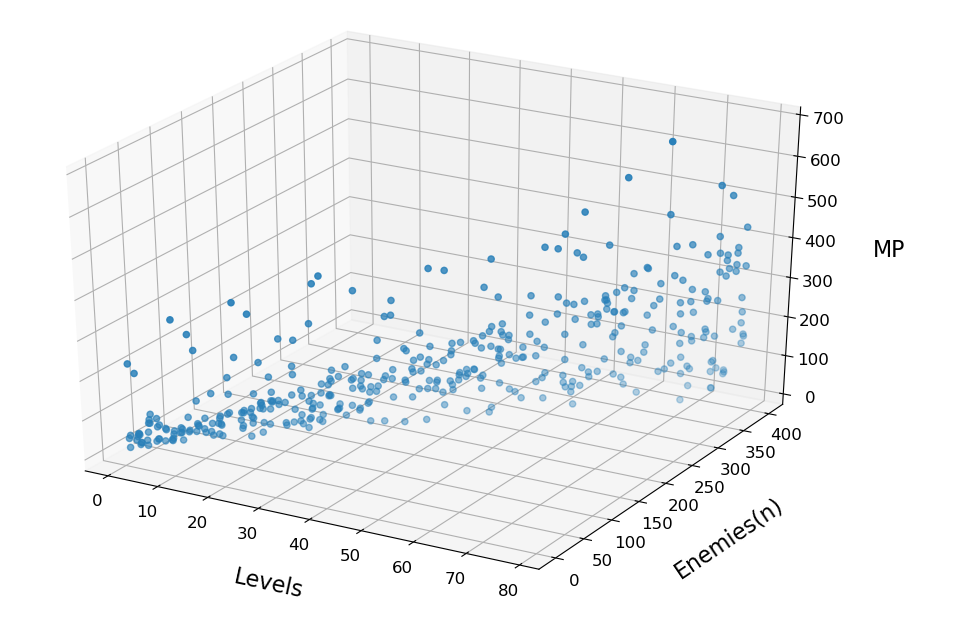
\includegraphics[scale=0.58]{img/EnemyMpDistrib.png}
	\caption{Distribusi \textit{stats} MP musuh.}
	\label{fig:enemy_mp_distrib}
\end{minipage} 
\end{figure}
\vspace{1ex}

Pada Gambar \ref{fig:enemy_str_distrib}, \ref{fig:enemy_mag_distrib}, \ref{fig:enemy_endr_distrib}, \ref{fig:enemy_spd_distrib} dan Gambar \ref{fig:enemy_luck_distrib} adalah pecahan dari Gambar \ref{fig:enemy_all_stats_distrib} secara berurutan diantaranya adalah \textit{Strength}, \textit{Magic}, \textit{Endurance}, \textit{Speed} dan \textit{Luck}.

\begin{figure} [!h]
	\begin{minipage}[t]{1.0\linewidth}
		\centering
		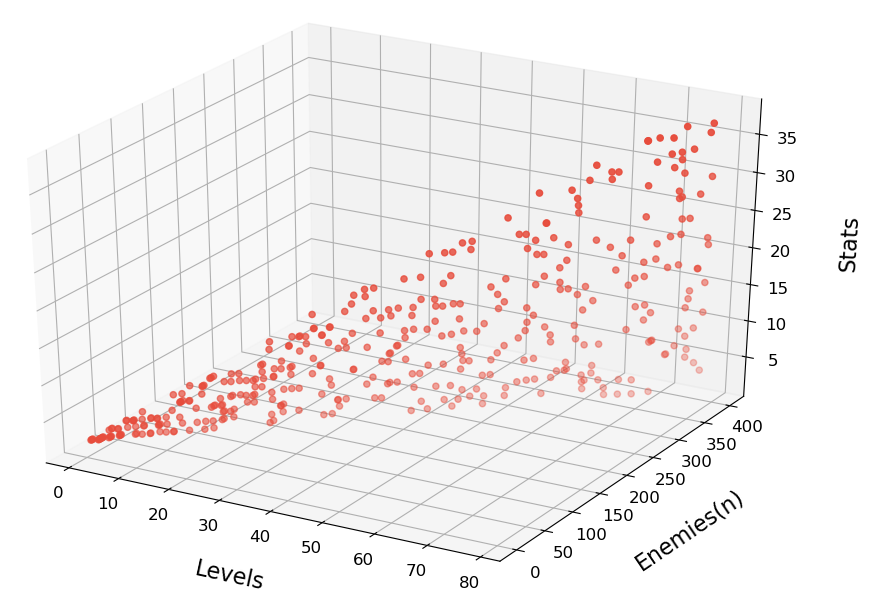
\includegraphics[scale=0.57]{img/EnemyStrengthDistrib.png}
		\caption{Distribusi \textit{Strength} musuh.}
		\label{fig:enemy_str_distrib}
		\vspace{2ex}
	\end{minipage}
	\vfill
	\begin{minipage}[t]{1.0\linewidth}
		\centering
		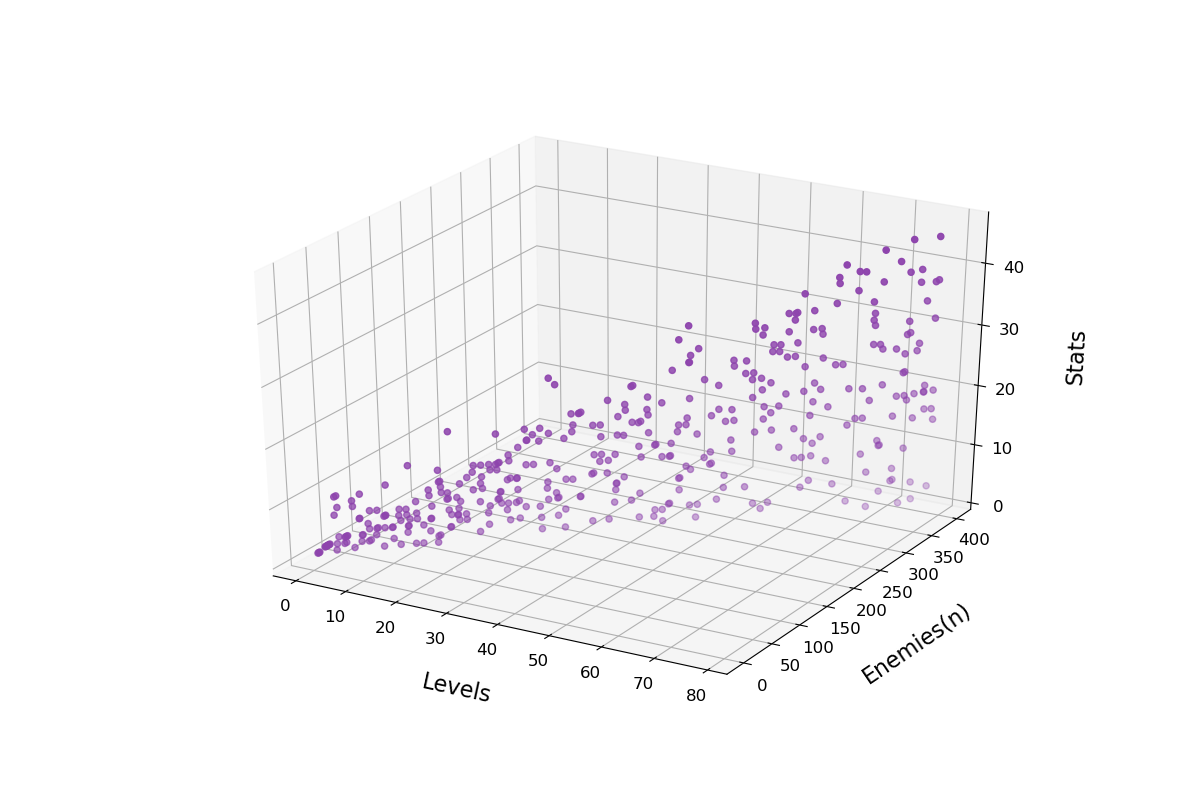
\includegraphics[scale=0.57]{img/EnemyMagicDistrib.png}
		\caption{Distribusi \textit{Magic} musuh.}
		\label{fig:enemy_mag_distrib}
	\end{minipage} 
\end{figure}

\begin{figure} [!h] \centering
	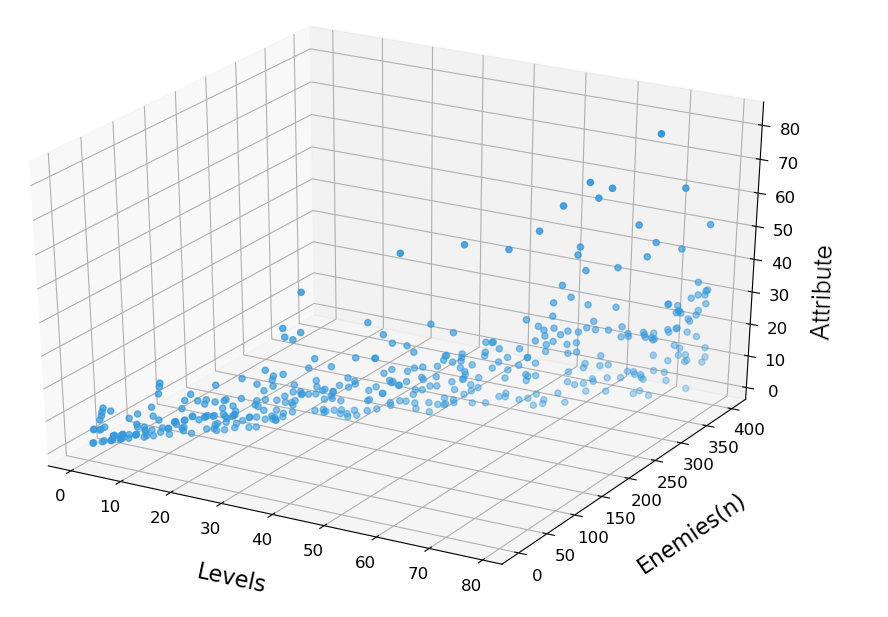
\includegraphics[scale=0.58]{img/EnemyEnduranceDistrib.png}
	\caption{Distribusi \textit{Endurance} musuh.}
	\label{fig:enemy_endr_distrib}
\end{figure}

\begin{figure} [!h] \centering
	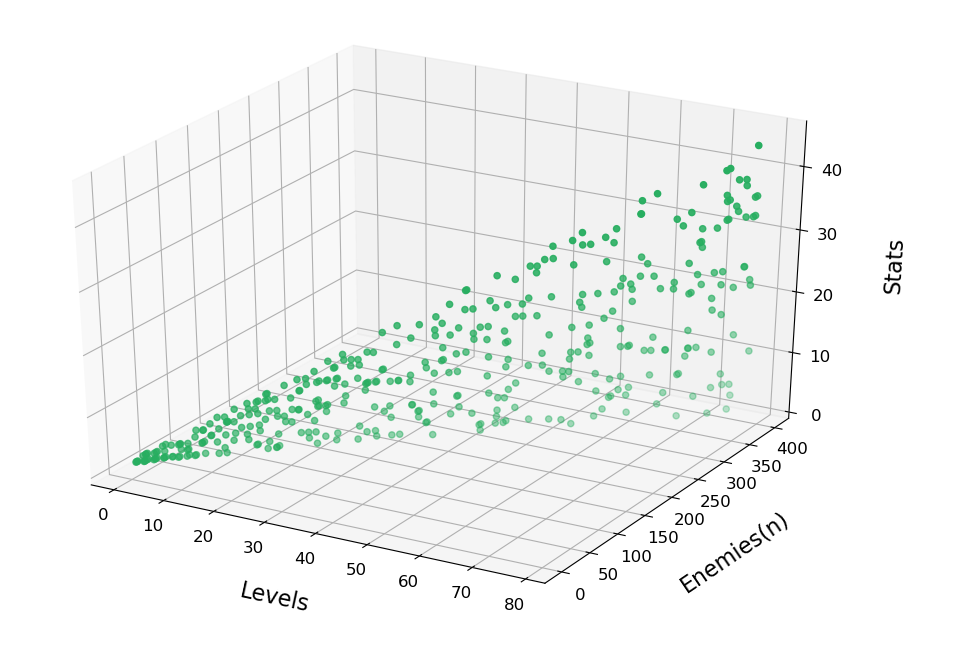
\includegraphics[scale=0.58]{img/EnemySpeedDistrib.png}
	\caption{Distribusi \textit{Speed} musuh.}
	\label{fig:enemy_spd_distrib}
\end{figure}

\begin{figure} [!h] \centering
	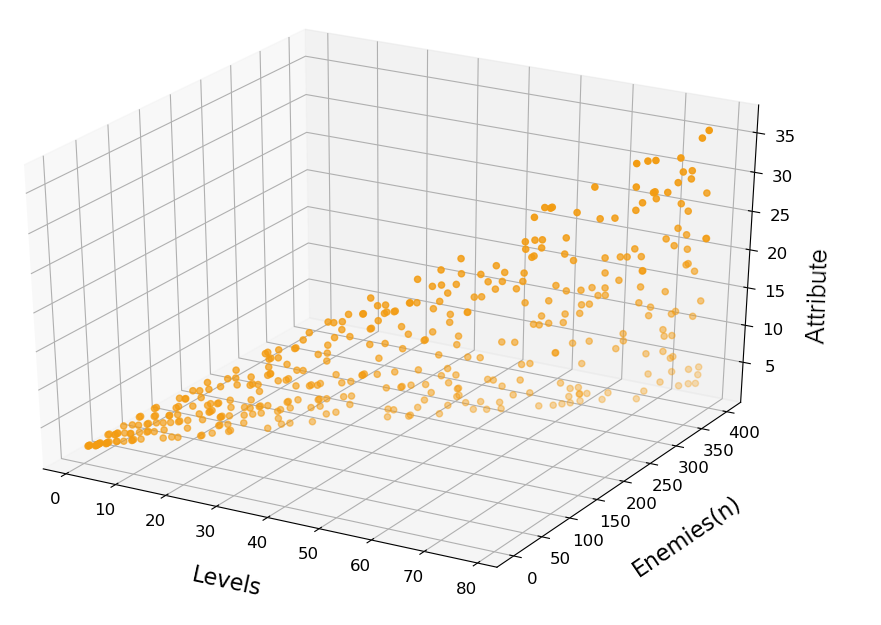
\includegraphics[scale=0.58]{img/EnemyLuckDistrib.png}
	\caption{Distribusi \textit{Luck} musuh.}
	\label{fig:enemy_luck_distrib}
\end{figure}